\documentclass[type=doctor]{thuthesis}
% 选项:
%   type=[bachelor|master|doctor|postdoctor], % 必选
%   secret,                                   % 可选
%   pifootnote,                               % 可选(建议打开)
%   openany|openright,                        % 可选,基本不用
%   arial,                                    % 可选,基本不用
%   arialtoc,                                 % 可选,基本不用
%   arialtitle                                % 可选,基本不用

% 所有其它可能用到的包都统一放到这里了,可以根据自己的实际添加或者删除。
\usepackage{thuthesis}

% 定义所有的图片文件在 figures 子目录下
\graphicspath{{figures/}}

% 可以在这里修改配置文件中的定义。导言区可以使用中文。
\def\myname{梁彧}
\newcommand\aap{A\&A}                % Astronomy and Astrophysics
\newcommand\aapr{A\&ARv}             % Astronomy and Astrophysics Review (the)
\newcommand\aaps{A\&AS}              % Astronomy and Astrophysics Supplement Series
\newcommand\actaa{Acta Astron.}      % Acta Astronomica
\newcommand\afz{Afz}                 % Astrofizika
\newcommand\aj{AJ}                   % Astronomical Journal (the)
\newcommand\ao{Appl. Opt.}           % Applied Optics
\newcommand\aplett{Astrophys.~Lett.} % Astrophysics Letters
\newcommand\apj{ApJ}                 % Astrophysical Journal
\newcommand\apjl{ApJ}                % Astrophysical Journal, Letters
\newcommand\apjs{ApJS}               % Astrophysical Journal, Supplement
%\newcommand\apspr{Astrophys.~Space~Phys.~Res.} % Astrophysics Space Physics Research
\newcommand\apss{Ap\&SS}             % Astrophysics and Space Science
\newcommand\araa{ARA\&A}             % Annual Review of Astronomy and Astrophysics
\newcommand\arep{Astron. Rep.}       % Astronomy Reports
\newcommand\aspc{ASP Conf. Ser.}     % ASP Conference Series
\newcommand\azh{Azh}                 % Astronomicheskii Zhurnal
\newcommand\baas{BAAS}               % Bulletin of the American Astronomical Society
\newcommand\bac{Bull. Astron. Inst. Czechoslovakia} % Bulletin of the Astronomical Institutes of Czechoslovakia
\newcommand\bain{Bull. Astron. Inst. Netherlands} % Bulletin Astronomical Institute of the Netherlands
\newcommand\caa{Chinese Astron. Astrophys.} % Chinese Astronomy and Astrophysics
\newcommand\cjaa{Chinese J.~Astron. Astrophys.} % Chinese Journal of Astronomy and Astrophysics
\newcommand\fcp{Fundamentals Cosmic Phys.}  % Fundamentals of Cosmic Physics
\newcommand\gca{Geochimica Cosmochimica Acta}   % Geochimica Cosmochimica Acta
\newcommand\grl{Geophys. Res. Lett.} % Geophysics Research Letters
\newcommand\iaucirc{IAU~Circ.}       % IAU Cirulars
\newcommand\icarus{Icarus}           % Icarus
\newcommand\japa{J.~Astrophys. Astron.} % Journal of Astrophysics and Astronomy
\newcommand\jcap{J.~Cosmology Astropart. Phys.} % Journal of Cosmology and Astroparticle Physics
\newcommand\jcp{J.~Chem.~Phys.}      % Journal of Chemical Physics
\newcommand\jgr{J.~Geophys.~Res.}    % Journal of Geophysics Research
\newcommand\jqsrt{J.~Quant. Spectrosc. Radiative Transfer} % Journal of Quantitiative Spectroscopy and Radiative Transfer
\newcommand\jrasc{J.~R.~Astron. Soc. Canada} % Journal of the RAS of Canada
\newcommand\memras{Mem.~RAS}         % Memoirs of the RAS
\newcommand\memsai{Mem. Soc. Astron. Italiana} % Memoire della Societa Astronomica Italiana
\newcommand\mnassa{MNASSA}           % Monthly Notes of the Astronomical Society of Southern Africa
\newcommand\mnras{MNRAS}             % Monthly Notices of the Royal Astronomical Society
\newcommand\na{New~Astron.}          % New Astronomy
\newcommand\nar{New~Astron.~Rev.}    % New Astronomy Review
\newcommand\nat{Nature}              % Nature
\newcommand\nphysa{Nuclear Phys.~A}  % Nuclear Physics A
\newcommand\pra{Phys. Rev.~A}        % Physical Review A: General Physics
\newcommand\prb{Phys. Rev.~B}        % Physical Review B: Solid State
\newcommand\prc{Phys. Rev.~C}        % Physical Review C
\newcommand\prd{Phys. Rev.~D}        % Physical Review D
\newcommand\pre{Phys. Rev.~E}        % Physical Review E
\newcommand\prl{Phys. Rev.~Lett.}    % Physical Review Letters
\newcommand\pasa{Publ. Astron. Soc. Australia}  % Publications of the Astronomical Society of Australia
\newcommand\pasp{PASP}               % Publications of the Astronomical Society of the Pacific
\newcommand\pasj{PASJ}               % Publications of the Astronomical Society of Japan
\newcommand\physrep{Phys.~Rep.}      % Physics Reports
\newcommand\physscr{Phys.~Scr.}      % Physica Scripta
\newcommand\planss{Planet. Space~Sci.} % Planetary Space Science
\newcommand\procspie{Proc.~SPIE}     % Proceedings of the Society of Photo-Optical Instrumentation Engineers
\newcommand\rmxaa{Rev. Mex. Astron. Astrofis.} % Revista Mexicana de Astronomia y Astrofisica
\newcommand\qjras{QJRAS}             % Quarterly Journal of the RAS
\newcommand\sci{Science}             % Science
\newcommand\skytel{Sky \& Telesc.}   % Sky and Telescope
\newcommand\solphys{Sol.~Phys.}      % Solar Physics
\newcommand\sovast{Soviet~Ast.}      % Soviet Astronomy (aka Astronomy Reports)
\newcommand\ssr{Space Sci. Rev.}     % Space Science Reviews
\newcommand\zap{Z.~Astrophys.}       % Zeitschrift fuer Astrophysik

\begin{document}

%%% 封面部分
\frontmatter
\thusetup{
  %******************************
  % 注意:
  %   1. 配置里面不要出现空行
  %   2. 不需要的配置信息可以删除
  %******************************
  %
  %=====
  % 秘级
  %=====
  secretlevel={秘密},
  secretyear={10},
  %
  %=========
  % 中文信息
  %=========
  ctitle={用巨洞研究宇宙学},
  cdegree={理学博士},
  cdepartment={物理系},
  cmajor={天体物理},
  cauthor={梁彧},
  csupervisor={莫厚俊教授},
  %cassosupervisor={陈文光教授}, % 副指导老师
  %ccosupervisor={某某某教授}, % 联合指导老师
  % 日期自动使用当前时间,若需指定按如下方式修改:
  % cdate={超新星纪元},
  %
  % 博士后专有部分
  %cfirstdiscipline={计算机科学与技术},
  %cseconddiscipline={系统结构},
  %postdoctordate={2009年7月——2011年7月},
  %id={编号}, % 可以留空: id={},
  %udc={UDC}, % 可以留空
  %catalognumber={分类号}, % 可以留空
  %
  %=========
  % 英文信息
  %=========
  etitle={Cosmology With Voids},
  % 这块比较复杂,需要分情况讨论:
  % 1. 学术型硕士
  %    edegree:必须为Master of Arts或Master of Science(注意大小写)
  %             “哲学、文学、历史学、法学、教育学、艺术学门类,公共管理学科
  %              填写Master of Arts,其它填写Master of Science”
  %    emajor:“获得一级学科授权的学科填写一级学科名称,其它填写二级学科名称”
  % 2. 专业型硕士
  %    edegree:“填写专业学位英文名称全称”
  %    emajor:“工程硕士填写工程领域,其它专业学位不填写此项”
  % 3. 学术型博士
  %    edegree:Doctor of Philosophy(注意大小写)
  %    emajor:“获得一级学科授权的学科填写一级学科名称,其它填写二级学科名称”
  % 4. 专业型博士
  %    edegree:“填写专业学位英文名称全称”
  %    emajor:不填写此项
  edegree={Doctor of Philosophy},
  edepartment={Department of Physics},
  emajor={Astropysics},
  eauthor={Liang Yu},
  esupervisor={Professor Mo Houjun},
  %eassosupervisor={Chen Wenguang},
  % 日期自动生成,若需指定按如下方式修改:
  % edate={December, 2005}
  %
  % 关键词用“英文逗号”分割
  ckeywords={巨洞, 宇宙学, 重子声波振荡, 星系红移巡天, 宇宙大尺度结构},
  ekeywords={void, cosmology, baryon acoustic oscillation, galaxy redshift survey, large scale structure of Universe.}
}

% 定义中英文摘要和关键字
\begin{cabstract}
  在暴涨时因量子涨落造成的宇宙原初密度扰动触发了重子-光子等离子体中的声波振荡。这些声学振荡导致了微波背景辐射各向异性功率谱和宇宙大尺度结构功率谱中的重子声波振荡特征尺度。重子声波振荡特征尺度可以被当作标准尺来测量宇宙中的距离。通过分析星系的成团性,重子声波振荡已经被成功的直接探测并深入研究。本工作首次提出如何通过宇宙低密度区域的成团性测量重子声波振荡。我们开发了能高效的在星系巡天数据中寻找巨洞的工具DIVE,并将其用于100组宇宙学大尺度结构数值模拟数据获得巨洞样本并研究巨洞的统计性质、空间分布、物质密度轮廓、动力学特性和相对物质密度场的bias。研究结果证实了样本中半径大于$16$ $h^{-1}$ Mpc的巨洞确实分布在宇宙低密度区域。我们通过计算不同半径巨洞中心的两点相关函数来测量重子声波振荡,并提出了一种不依赖宇宙学模型的估算重子声波振荡信号信噪比的方法,用以寻找重子声波振荡信号信噪比最大的巨洞子样本。用所有半径大于$16$ $h^{-1}$ Mpc的巨洞作为样本可以得到信噪比最高的重子声波振荡信号。我们进一步研究了如何用SDSS-III/BOSS CMASS DR11样本中光锥模拟星系表的巨洞数据探测重子声波振荡信号,提出了构建计算巨洞两点相关函数时所需要的随机样本的方法。最终我们使用BOSS CMASS DR11观测数据中的巨洞计算两点相关函数,并通过1024组光锥模拟星系表的巨洞数据估算协方差矩阵,首次成功的使用观测数据中的巨洞获得3.2$\sigma$置信度的重子声波振荡信号。
\end{cabstract}

% 如果习惯关键字跟在摘要文字后面,可以用直接命令来设置,如下:
% \ckeywords{\TeX, \LaTeX, CJK, 模板, 论文}

\begin{eabstract}
  We investigate the necessary methodology to optimally measure the baryon acoustic oscillation (BAO) signal from voids, based on galaxy redshift catalogues. 
  To this end, we study the dependency of the BAO signal on the population of voids classified by their sizes. 
  We find for the first time the characteristic features of the correlation function of voids including the first robust detection of BAOs in mock galaxy catalogues. These show an anti-correlation around the scale corresponding to the smallest size of voids in the sample (the void exclusion effect), and  dips at both sides of the BAO peak, which can be used to determine the significance of the BAO signal without any priori model.
  Furthermore, our analysis demonstrates that there is a scale dependent bias for different populations of voids depending on the radius, with the peculiar property that the void population with the largest BAO significance corresponds to tracers with approximately zero bias on the largest scales.
  We further investigate the methodology on an additional set of 1,000 realistic mock galaxy catalogues reproducing the SDSS-III/BOSS CMASS DR11 data, to control the impact of sky mask and radial selection function. Our solution is based on generating voids from randoms including the same survey geometry and completeness, and a post-processing cleaning procedure in the holes and at the boundaries of the survey.
  The methodology and optimal selection of void populations validated in this work have been used to perform the first BAO detection from voids in observations. We use the luminous red galaxies sample from BOSS/SDSS-III CMASS DR11 to unveil a 3.2$\sigma$ BAO detection from vodis for the first time in observation.
\end{eabstract}

% \ekeywords{\TeX, \LaTeX, CJK, template, thesis}

% 如果使用授权说明扫描页,将可选参数中指定为扫描得到的 PDF 文件名,例如:
% \makecover[scan-auth.pdf]
\makecover

%% 目录
\tableofcontents

%% 符号对照表
\begin{denotation}[3cm]
\item[void] 巨洞
\item[SDSS] 斯隆数字化巡天 (Sloan Digital Sky Survey)
\item[DR] Data Release
\item[LRG] 亮红星系 (Luminous Red Galaxy)
\item[2PCF] 两点相关函数 (two-point correlation function)
\item[2dFGRS] 2度视场星系红移巡天 (Two Degree Filed Galaxy Redshift Survey)
\item[BAO] 重子声波振荡 (baryon acoustic oscillation)
\item[BOSS] 重子振荡光谱巡天 (Baryon Oscillation Spectroscopic Survey)
\item[Quasar] 类星体
\item[CMB] 宇宙微波背景辐射 (cosmic microwave background)
\item[SNIa] Ia 型超新星 (type Ia supernova)
\item[DESI]	The Dark Energy Spectroscopic Instrument
\item[DES] The Dark Energy Survey
\item[J-PAS] The Javalambre Physics of The Accelerating Universe Astrophysical Survey
\item[4MOST] The 4-metre Multi-Object Spectroscopic Telescope
\item[EUCLID] 欧几里得空间望远镜
\item[PFS] Subaru Prime Focus Spectroscopy
\item[WFIRST] 大视场红外巡天望远镜 (Wide-Field Infrared Survey Telescope)
\item[CfA] CfA 红移巡天 (The Center of Astrophysics redshift survey)
\item[IRAS] 红外天文卫星 (The Infrared Astronomical Satellite)
\item[LasCampanas] 拉斯坎帕纳斯红移巡天 (The Las Campanas Redshift Survey)
\item[PSCz] 点源星表红移巡天 (The IRAS Point Source Catalog Redshift Survey)
\item[DEEP2] The Deep Extragalactic Evolutionary Probe 2
\item[2MRS] The 2MASS Redshift Survey
\item[VIMOS] The Visible Multi-Object Spectrograph
\item[PDF] 概率分布函数 (probability distribution functions)
\item[$\sigma_8$] 在$8\, h^{-1}\, \mathrm{Mpc}$的球形区域内,总物质质量相对平均值的涨落方均根
\item[AP test] 阿尔科克-帕金斯基检验 (Alcock-Paczy$\acute{\rm n}$ski test)
\item[SZ effect] 萨克斯-沃尔夫效应 (The Sachs-Wolfe effect)
\item[2PCF] 两点相关函数 (two-Point Correlation Function)
\item[DT] 德劳内三角剖分 (Delaunay Triangulation)
\item[DIVE] Delaunay trIangulation Void findEr
\item[$H_0$] 哈勃常数 ($H_0 \equiv 100\,h\,\mathrm{km}\,\mathrm{s}^{-1}\mathrm{Mpc}^{-1}$)
\item[$h$] 无量纲的哈勃参数
\item[6dFGS] 6度视场星系巡天 (The Six Degree Field Galaxy Survey)
\item[$z$] 红移
\item[ELG] 发射线星系 (Emission Line Galaxies)
\item[$c$] 光速
\item[$D_A(z)$] 红移z处的角直径距离 (angular diameter distance)
\item[$H(z)$] 哈勃参量 (Hubble parameter)
\item[$D_V(z)$] $D_V(z) \equiv \left[ cz (1+z)^2 D_A(z)^2 H^{-1}(z) \right]^{1/3}$
%\item[CMASS] 
\item[SML] 平滑长度 (SMoothing Length)
\item[$\vec{\Psi}$] 位移场 (the displacement field)
\item[$\delta$] 密度反差 (density contrast)
\item[$b$] bias
\item[$a$] 宇宙标度因子 (scale factor of the universe)
\item[$D(a)$] 宇宙线性增长函数 (linear growth function)
\item[$\Omega_{M}$] 物质密度相对临界密度的比值
\item[$f$] 宇宙大尺度结构的线性增长率 (linear growth rate)
\item[RA] Right Ascension
\item[DEC] Declination
\item[$\alpha$] 尺度膨胀参数 (the scale dilation parameter)
\item[fid] 基准宇宙学模型
\item[$\xi$] 相关函数
\item[PATCHY] The PerturbAtion Theory Catalogue generator of Halo and galaxY
\item[$n_s$] spectral tilt
\item[RSD] 红移畸变效应 (redshift space distortion)
\item[HAM] Halo Abundance Matching
\item[SGC] Southern Galactic Cap
\item[NGC] Northern Galactic Cap
\item[$T_{ij}$] 潮汐张量
\item[$\phi$] 引力势
\item[$S/N$] 信噪比
\end{denotation}



%%% 正文部分
\mainmatter
\chapter{引言}
\label{cha:intro}

在十年前,通过计算斯隆数字化巡天~\cite{York2000} (Sloan Digital Sky Survey,SDSS) DR3 亮红星系(Luminous Red Galaxy,LRG)~\cite{Eisenstein2001}样本的两点相关函数(two-point correlation function, 2PCF)和 2度视场星系红移巡天~\cite{Colless2001}(Two Degree Filed Galaxy Redshift Survey,2dFGRS)星系样本的功率谱(power spectrum),重子声波振荡(baryon acoustic oscillation,BAO)首次被直接探测到~\cite{Eisenstein2005,Cole2005}。
此后SDSS的巡天观测以及其他星系红移巡天(galaxy redshift surveys)项目的成果大大提高了对BAO特征尺度测量的精确性~\cite{Percival2010,Blake2011,Beutler2011,Drinkwater2010,White2011,Eisenstein2011,Dawson2013,Anderson2014441,Ross2015}。
重子振荡光谱巡天~\cite{Dawson2013}(Baryon Oscillation Spectroscopic Survey,BOSS)是斯隆数字化巡天三期~\cite{Eisenstein2011}(SDSS-III)的重要组成部分,该项目首次成功利用莱曼$\alpha$森林(Lyman $\alpha$ forest)的自相关函数(auto-correlation function),和莱曼$\alpha$森林与高红移类星体(Quasar)的互相关函数(cross-correlation function)探测到BAO信号~\cite{Busca2013,Slosar2013,Font-Ribera2014,Delubac2015}。

因为BAO的特征尺度受系统误差影响较小,能在较高红移被精确测量,其大小可以从第一原理(first principle)出发用基本的宇宙学参数计算得出,所以BAO成为精确测量宇宙膨胀历史和研究宇宙大尺度结构形成演化的最好探针之一。目前将BAO和宇宙微波背景辐射(cosmic microwave background,CMB)结合起来对宇宙学参数的限制能力已经超越Ia型超新星(type Ia supernova,SNIa)与CMB的组合~\cite{ABB14}。
未来的几个大型巡天项目和望远镜,包括The Dark Energy Spectroscopic Instrument~\cite{bigboss2011}(DESI)、The Dark Energy Survey~\cite{des2013}(DES)、大口径全天巡视望远镜~\cite{lsst2012}(The Large Synoptic Survey Telescope,LSST)、The Javalambre Physics of The Accelerating Universe Astrophysical Survey~\cite{jpas2014}(J-PAS)、The 4-metre Multi-Object Spectroscopic Telescope~\cite{4most}(4MOST)、欧几里得空间望远镜~\cite{euclid2009}(EUCLID)、Subaru Prime Focus Spectroscopy~\cite{Tamura2016}(PFS)和大视场红外巡天望远镜\footnote{\url{http://wfirst.gsfc.nasa.gov}}(Wide-Field Infrared Survey Telescope,WFIRST),都把精确测量BAO特征尺度作为其重要的科学目标之一。

巨洞是宇宙大尺度结构中占据大部分空间的低密度区域,里面一般不存在大质量星系。The Giant Bo\"otes voids~\cite{KOS81}是首次被观测到的巨洞。随后的星系巡天观测中,如CfA红移巡天~\cite{LGH86,VGP94}(The Center of Astrophysics redshift survey)、红外天文卫星~\cite{EP97}(The Infrared Astronomical Satellite,IRAS)、拉斯坎帕纳斯红移巡天~\cite{MAE00}(The Las Campanas Redshift Survey,LasCampanas)、点源星表红移巡天~\cite{PB02}(The IRAS Point Source Catalog Redshift Survey,PSCz)、2dFRGS~\cite{CCG04,HV04,Patiri2006HB}、The Deep Extragalactic Evolutionary Probe 2~\cite{CCW05}(DEEP2)、The 2MASS Redshift Survey~\cite{NKH14}(2MRS)、SDSS~\cite{Platen2011,VBT12,PVH12,NH14,SLW14,BKH15}和The Visible Multi-Object Spectrograph~\cite{Micheletti02014}(VIMOS),越来越多的巨洞被观测到。巨洞的存在显示了宇宙在大尺度上并不非常均匀,而是以网状的结构(cosmic web structure)存在,巨洞是宇宙网状结构中很明显的一部分。

基于暗物质密度场的宇宙学演化,可以从理论的角度研究巨洞~\cite{Doroshkevich1970,Zeldovich1970,Hahn2007}。而通过宇宙学大尺度结构数值模拟也可以证明巨洞的存在和演化~\cite{SW04,Colberg2005, 2006MNRAS.367.1629S, Platen2007, Neyrinck2008, Forero-Romero2009, 2012MNRAS.425.2049H, 2013MNRAS.429.1286C}。巨洞是限制宇宙学参数或检验不同引力理论的探针。巨洞的数密度(number density)分布和概率分布函数(probability distribution functions,PDF)可以用来限制$\sigma_8$和$\Omega_m h$~\cite{BPP09,2015arXiv151104075S}。巨洞的统计性质还可以用作其他宇宙学研究~\cite{W79,PP86,B90,EEG91,BL02}。巨洞堆叠起来之后的形状可以用阿尔科克-帕金斯基检验(Alcock-Paczy$\acute{\rm n}$ski test,AP test)限制暗能量模型~\cite{PL07,LW10,Pisani2015PRD},巨洞的形状还可以检验动力学暗能量模型~\cite{B12}(dynamical dark energy model)和耦合暗能量模型~\cite{L11}(coupled dark energy model)。巨洞的统计性质还可以用来检验不同的引力理论~\cite{MS09,LZK12,CC13,LCC15,Cai2015}或研究萨克斯-沃尔夫效应(The Sachs-Wolfe effect,SZ 效应)~\cite{GNS08,ILD13,Cai2014,HNG15,PLANCKISW14}。

曾有人研究过巨洞的两点相关函数,但是因为那些研究中巨洞的数密度非常低,所以用那些定义巨洞的方法不可能探测到有效的BAO信号~\cite{Padilla2005,Patiri2006372,VBT12,CC13,CJS15}。在我们的研究中引入了一种全新的定义巨洞的方式:对在三维空间离散分布的星系或暗物质晕(dark matter halo)做德劳内三角剖分(Delaunay Triangulation,DT)而得到的四面体所确定的空心球定义为德劳内三角剖分巨洞(DT巨洞)。同时我们开发了一款能够非常高效的寻找这些DT巨洞的工具DIVE(Delaunay trIangulation Void findEr)。用DIVE所得到的DT巨洞可以让我们有机会获得宇宙低密度区域的位置并研究其成团性,而用这种定义巨洞的方式能否探测到一个高置信度的BAO信号,以及通过DT巨洞探测到的BAO信号相对于直接用星系成团性所测的BAO信号有什么区别将成为本文的主要研究内容。直觉上,相比星系或星系团,巨洞所遭受的引力作用应该比较小,因此巨洞的中心理应受非线性演化影响较小,巨洞的体积在演化中会以球对称的方式变大~\cite{SW04}。所以巨洞应该是一种更加理想的用以研究宇宙最初的密度涨落的探针。

本文的结构如下:
第~\ref{cha:bao} 章综述了用星系测量BAO的研究;
%第~\ref{cha:void} 章总结了不同的寻找巨洞的方式及相应的研究;
第~\ref{cha:data} 章介绍了本文研究中所使用的数据;
第~\ref{cha:DIVE} 章展示了DIVE及DT巨洞的统计性质;
第~\ref{cha:voidbao} 章研究了如何从DT巨洞中探测BAO信号;
%第~\ref{cha:recon} 章讨论了BAO信号重构分别对星系和巨洞BAO信号的影响;
第~\ref{cha:summary} 章总结了全文的主要结论。


\chapter{重子声波振荡}
\label{cha:bao}

\section{引言}
在暴涨时因量子涨落造成的宇宙原初密度扰动触发了重子-光子等离子体中的声波振荡。这些声学振荡造成了微波背景辐射各向异性功率谱和宇宙大尺度结构功率谱中的特征尺度~\cite{Sakharov1966,Peebles1970,Sunyaev1970,Blake2003,Seo2003}。这个特征尺度就是本文所主要研究的BAO特征尺度,它可以作为宇宙中的标准尺(cosmological standard ruler)来研究宇宙的膨胀历史和检验不同的宇宙学模型。

最初人们通过CMB~\cite{Bond1984,Bond1987,Jungman1996,Hu1996s,Hu1996w,Hu1997}和物质功率谱~\cite{Kamionkowski1994,Jungman1996,Hu1996s,Eisenstein1998,Meiksin1999}来研究原初宇宙中的声学振荡。2dFGRS早期数据~\cite{Percival2001,Efstathiou2002,Percival2002}和艾贝尔星系团表~\cite{Miller1999}(the Abell/ACO cluster sample)的功率谱中显示了声学振荡存在的一些迹象,但是第一次直接探测到清晰可靠的BAO信号~\cite{Eisenstein2005,Cole2005}来自于对SDSS低红移星系和2dFGRS数据的成团性研究。文献 ~\inlinecite{Eisenstein2005}计算了SDSS所观测的3816平方度天区在红移范围$0.16 < z < 0.47$内亮红星系的两点相关函数,探测到显著性为$3.4\sigma$的BAO信号。文献 ~\inlinecite{Cole2005}通过计算2dFGRS最终观测数据的功率谱证实了BAO的存在并得到对哈勃常数$H_0$ 准确度为4.1\%的测量。

文献 ~\inlinecite{Eisenstein2005}和文献 ~\inlinecite{Cole2005}首次成功的直接探测到BAO信号以后,对BAO特征尺度的测量精度被接下来的大型星系红移巡天项目大大提高。文献 ~\inlinecite{Percival2010}结合了2dFGRS最终观测数据和SDSS-II的数据,并利用FKP方法~\cite{Feldman1994},测得在红移$z \approx 0.275$处精确度为2.7\%的BAO特征尺度。文献 ~\inlinecite{Eisenstein2007recon}基于数值模拟数据,首次在理论上提出重构BAO信号的方法(BAO reconstruction methods)以消除非线性演化对BAO信号影响。随后文献 ~\inlinecite{Padmanabhan2012}将BAO信号重构改进,使其适用于观测数据(SDSS DR7 LRG样本),利用这一方法BAO特征尺度的测量精度被提高到1.9\%。6度视场星系巡天~\cite{Jones2009}(The Six Degree Field Galaxy Survey,6dFGS)观测了17000平方度范围内红移$z \sim 0.1$处的星系,文献 ~\inlinecite{Beutler2011}利用这些数据得到$2.4\sigma$置信度的BAO信号及精确度为4.5\%的BAO特征尺度。The WiggleZ survey~\cite{Drinkwater2010}利用英澳望远镜(the Anglo-Australian Telescope)观测了红移$0.4 < z < 1.0$内的发射线星系(Emission Line Galaxies,ELG),测到精确度为3.8\%的BAO特征尺度~\cite{Blake2011}。BOSS/SDSS-III计划利用红移$0.2 < z < 0.7$内的星系红移巡天数据取得对BAO特征尺度精确度为1\%的测量,并首次提出利用莱曼$\alpha$森林的吸收线分析$z \sim 2.5$附近中性氢的成团性,和莱曼$\alpha$森林与高红移类星体的互相关函数以探测BAO信号~\cite{White2003,McDonald2007}。
文献 ~\inlinecite{Anderson2014441}利用BOSS/SDSS-III CMASS DR10和DR11样本测量了球对称BAO特征尺度$D_V(z)$(the isotropic BAO scale),其在红移红移$z=0.32$处精确度为2.0\%和红移$z=0.57$处精确度为1.0\%。$D_V(z)$的定义为
\begin{equation}
D_V(z) \equiv \left[ cz (1+z)^2 D_A(z)^2 H^{-1}(z) \right]^{1/3},
\end{equation}
其中$c$是光速,$z$是红移,$D_A(z)$是角直径距离(angular diameter distance),$H(z)$是哈勃参量(Hubble parameter)。文献 ~\inlinecite{Okumura2008,Chuang2012}首次提出测量非球对称BAO特征尺度的方法,文献 ~\inlinecite{Anderson2014441}用BOSS/SDSS-III CMASS DR11样本也测量了非球对称BAO特征尺度,在红移$z=0.57$处实现对$D_A(z)$ 精确度为1.4\%和$H(z)$ 精确度为3.5\%的测量,$D_A(z)$与$H(z)$之间相关性系数(correlation coefficient)为$0.539$。
在有效红移$z \sim 2.34$处,文献 ~\inlinecite{Delubac2015}利用BOSS/SDSS-III CMASS DR11样本的莱曼$\alpha$森林样本得到对$H(z)$ 精确度为2.6\%和对$D_A(z)$ 精确度为5.4\% 的测量,文献 ~\inlinecite{Font-Ribera2014}利用BOSS/SDSS-III CMASS DR11样本中莱曼$\alpha$森林和高红移类星体的互相关函数得到对$H(z)$ 精确度为3.3\%和对$D_A(z)$ 精确度为3.7\% 的测量。
文献 ~\inlinecite{Alam2016}使用BOSS/SDSS-III最终的DR12样本,
在红移$z=0.32$处,对$D_V(z)$、$D_A(z)$和$H(z)$的测量精度分别达到1.1\%、1.6\%和2.9\%,
在红移$z=0.57$处,对$D_V(z)$、$D_A(z)$和$H(z)$的测量精度分别达到1.0\%、1.6\%和2.5\%。
文献 ~\inlinecite{Bautista2017}利用BOSS/SDSS-III DR12样本的莱曼$\alpha$森林样本,在红移$z=2.33$处,对$D_A(z)$和$H(z)$的测量精度分别达到5.6\%和3.4\%。

\section{重构BAO信号}
\label{sec:baorecon}

在文献 ~\inlinecite{Eisenstein2005}通过分析SDSS星系样本成团性首次成功的直接探测到BAO信号之后,文献 ~\inlinecite{Eisenstein2007recon}使用宇宙大尺度结构数值模拟数据首次在理论上提出重构BAO信号的方法并展示其效果~\cite{Eisenstein2007b,Padmanabhan2009}。
关于BAO信号重构的一些其他早期工作也证实了此方法可以提高BAO特征尺度的测量精度。
文献 ~\inlinecite{Padmanabhan2009}基于拉格朗日微扰论(Lagrangian perturbation theory),从理论的角度分析了BAO信号重构的方法。
文献 ~\inlinecite{Noh2009}将文献 ~\inlinecite{Padmanabhan2009}的理论工作扩展到偏袒的天体(biased tracer)。
文献 ~\inlinecite{White2015}基于Zeldovich近似(Zeldovich Approximation)给出了BAO信号重构后(post-reconstruction)相关函数的公式。
文献 ~\inlinecite{Xu2012}研究了BAO重构对球对称BAO信号的影响,文献 ~\inlinecite{Anderson2012}研究了BAO重构对非球对称BAO信号的影响。

文献 ~\inlinecite{Padmanabhan2012}改进了文献 ~\inlinecite{Eisenstein2007recon}的方法,使得重构BAO信号的算法可以用于观测数据。此后BAO信号重构被广泛用于各种星系红移巡天的星系成团性分析中~\cite{Anderson2012,Anderson2014439,Kazin2014,Tojeiro2014,Burden2015,Ross2015},对于BAO特征尺度的测量精度最高可以有45\%的提升。

BAO重构的算法包括以下几个步骤:
\begin{description}
\item[1.] 暗物质晕或星系是相对物质密度场有偏袒的天体,根据暗物质晕或星系在空间中的离散分布并利用插值算法(如Nearest Grid Point(NGP)或Cloud In Cell(CIC)),可以估算出物质密度场。
\item[2.] 为了去除非线性效应在小尺度的噪音,需要对上一步所估算的密度场进行平滑长度(SMoothing Length)为SML的高斯过滤(Gaussian filter),被过滤的来自小尺度的高频噪音对大尺度星系巡天的影响微乎其微。
\item[3.] 用Zeldovich近似求位移场(the displacement field)$\vec{\Psi}$的一阶近似解。在实空间(real space),求解的方程为
\begin{equation} \label{EQ:psireal}
\nabla \cdot \vec{\Psi}=-\frac{\delta_g}{b}
\end{equation}
其中$\vec{\Psi}$是拉格朗日位移场(Lagrangian displacement field),$\delta_{g}$星系的密度涨落,$b$是星系的偏袒(galaxy bias)。在红移空间(redshift spcae)拉格朗日位移场与密度场的关系变为
\begin{equation} \label{EQ:displacement}
\nabla \cdot \vec{\Psi}+f \nabla \cdot (\vec{\Psi} \cdot \hat{s}) \hat{s}=-\frac{\delta_g}{b}
\end{equation}
其中
%$\hat{s}$是星系的矢量位置,
$\hat{s}$是视线方向(line of sight direction),$f$是宇宙大尺度结构的线性增长率(linear growth rate),
\begin{equation}
f \equiv d \ln D(a)/d \ln a \sim\! \Omega_{M}^{0.55}
\end{equation}
其中$a$是宇宙标度因子(scale factor of the universe),$D(a)$是宇宙线性增长函数(linear growth function),$\Omega_{M}$物质密度(matter density)相对临界密度(critical density)的比值~\cite{Carroll1992,Linder2005}。将暗物质晕或星系移动$-\vec{\Psi}$,如果是在红移空间还需要将暗物质晕或星系额外移动$-f (\vec{\Psi} \cdot \hat{s}) \hat{s}$。在红移空间,公式~(\ref{EQ:displacement})中额外移动的部分可以在线性理论(linear theory)的尺度上消除红移畸变(redshift space distortion,RSD)效应。这些经过位移的暗物质晕或星系在后文中被表示为D。
\item[4.] 生成一些均匀随机分布的物体作为随机样本,这些随机样本在后文用R表示。
\item[5.] 将R复制一份,并按照$-\vec{\Psi}$移动这些样本。因为这些随机样本并没有遭受RSD效应的影响,所以在红移空间不需要做额外的移动。这些经过位移的随机样本在后文用S表示。
\end{description}

理论上应该对功率谱做傅立叶变换计算得到2PCF,但是因为星系红移巡天数据的体积有限,以及巡天观测存在很多限制,所以对功率谱做傅立叶变换计算所得到的2PCF并不是十分准确。\inlinecite{Landy1993}提出的估算2PCF的方法(The Landy \& Szalay estimator)相对其他方法~\cite{Peebles1974,Hewett1982,Davis1983,Hamilton1993}更加准确,因此被广泛应用。The Landy \& Szalay estimator的表达式为:
\begin{equation} \label{EQ:lsestimator}
\xi (s)=\frac {DD(s)-2DR(s)+RR(s)} {RR(s)}
\end{equation}
其中$DD(s)$、$DR(s)$和$RR(s)$是对应样本之间在$s$距离上归一化后的样本对数。而估算post-reconstruction样本的2PCF时需要对The Landy \& Szalay estimator做一些更改:
\begin{equation} \label{EQ:postreconcf}
\xi (s)=\frac {DD(s)-2DS(s)+SS(s)} {RR(s)}
\end{equation}
其中$DD(s)$、$DS(s)$、$SS(s)$和$RR(s)$也是对应样本之间在$s$距离上归一化后的样本对数。

\section{测量球对称BAO信号}
\label{sec:isobao}

原初宇宙中的声学振荡在重子-光子等离子体中以声速传播。但是随着宇宙的膨胀,宇宙的温度逐渐降低,CMB形成时电子与质子或原子核复合,重子-光子等离子体不复存在,声学视界的大小$r_d$逐渐固定下来,成为可以测量宇宙距离的标准尺。球对称BAO特征尺度就是$r_d$在球面上的平均值,可以通过$D_V(z)/r_d$进行测量。

星系红移巡天所观测到宇宙的体积是锥形的,一般被称作光锥(light-cone)。光锥中星系的坐标为球坐标系(RA,DEC,z),其中RA为Right Ascension,DEC为Declination,z是红移。需要假设一个基准宇宙学模型才能将星系在天球的角度位置和红移转换成共动距离(comoving distance)。而巡天观测中需要假设基准宇宙学模型并测量尺度膨胀参数(the scale dilation parameter),$\alpha$,来测量BAO特征尺度:
\begin{equation} \label{EQ:alpha}
\alpha \equiv \frac{D_V(z)r_{d}^{\rm fid}}{D^{\rm fid}_V(z) r_d} 
\end{equation}
其中上标${\rm fid}$表示基准宇宙学模型相对应的参数。${r_{d}^{\rm fid}}/{r_{d}}$是BAO特征尺度在共动距离单位下基准宇宙学模型与真实观测的比值。${D_V(z)}/{D_V^{\rm fid}(z)}$是真实观测数据和基准宇宙学模型不同的球面平均的比值。

\subsection{拟合相关函数的理论模型}
基于线性理论可以构建一个拟合星系非线性相关函数的模版并以此测量BAO特征尺度。BAO特征尺度的相对大小由拟合相关函数的模版函数$\xi^{fit}(s)$里的$\alpha$测量,$\alpha$表示基准宇宙学模型与真实观测值比例。$\xi^{fit}(s)$的表达式为
\begin{equation} \label{EQ:xifit}
\xi^{fit}(s) = B^{2} \xi_{m}(\alpha s) + A(s)\,,
\end{equation}
其中$B$是归一化因子,$\xi_{m}$是基于线性理论推导得出的线性相关函数模型,$A(s)$用来拟合非线性相关函数的整体轮廓并消除有尺度依赖的偏袒因子(scale-dependent bias factor)的影响:
\begin{equation}
A(s)  = \frac{a_1}{s^2} + \frac{a_2}{s} + a_3
\end{equation}
其中 $a_1$,$a_2$和$a_3$是待拟合参数,一般不关心其具体数值,所以也被称作多余参数(nuisance parameters)。基于线性理论推导得出的线性相关函数模型$\xi_{m}$的表达式为
\begin{equation} \label{EQ:xim}
\xi_m(r) = \int \frac{k^2dk}{2\pi^2}P_m(k) \mathfrak{j}_0 (kr)\mathrm{e}^{-k^2a^2},
\end{equation}
其中$P_m(k)$是功率谱模型,$\mathfrak{j}_0$是第一类零阶贝塞尔函数(the 0th-order spherical Bessel function of the first kind)
\begin{equation}
\mathfrak{j}_0 (x) =  \frac{\sin{x}}{x}
\end{equation}
公式~(\ref{EQ:xim})中
%的参数$a$是振荡变换核函数$\mathfrak{j}_0 (ks)$的高频阻尼(high-$k$ damping)的额外高斯项。
参数$a$的存在可以使数值积分更好的收敛,并且取$a = 1 h^{-1}{\rm\;Mpc}$较为合理~\cite{Xu2012}。功率谱模型的表达式为
\begin{equation}
P_{\mathrm{m}} (k) = [P_{\mathrm{lin}} (k) - P_{\mathrm{smooth}} (k)] \mathrm{e}^{-k^2 \Sigma^2_{\mathrm{nl}} / 2} + P_{\mathrm{smooth}} (k)
\end{equation}
其中$P_{\mathrm{lin}} (k)$是用CAMB~\cite{CAMB2000}计算的线性功率谱,$P_{\mathrm{smooth}} (k)$是用文献 ~\inlinecite{Eisenstein1998}内提供的方法计算的没有声学振荡的功率谱,$\Sigma_{\mathrm{nl}}$是线性BAO信号的标准高斯阻尼因子(the standard Gaussian damping factor)。文献 ~\inlinecite{Xu2012}发现$\Sigma_{\mathrm{nl}}$的值变动时对最终结果影响很小,$\Sigma_{\mathrm{nl}}$的值被固定为$8 h^{-1}\mathrm{Mpc}$。但是文献 ~\inlinecite{Noh2009}的研究表明不固定$\Sigma_{\mathrm{nl}}$时,也就是将$\Sigma_{\mathrm{nl}}$作为一个自由的拟合参数时,可以取得更优的拟合结果。本工作拟合BAO信号时,$\Sigma_{\mathrm{nl}}$是一个被限制在较大范围内的待拟合参数。

\subsection{协方差矩阵}

利用很多组模拟数据~\cite{Hamilton2006,Takahashi2009,Xu2012}(mock catalogues),或者基于微扰论~\cite{Scoccimarro2002},都可以得到协方差矩阵。用微扰论得到的协方差矩阵不够准确。虽然用很多(成百上千)组模拟数据所得到的协方差矩阵仍然不是十分精确,但这样得到的协方差矩阵相比用微扰论得到的结果要可靠很多。

为了方便与他人已经发表的工作进行对比验证,在我们的工作中采用最常用的方法,协方差矩阵是通过很多模拟数据计算推导的:
\begin{equation}
C_{s,ij} = \frac{1}{N_m - 1} \sum^{N_m}_{k = 1} [\xi_k(s_i) - \bar{\xi}(s_i)][\xi_k(s_j) - \bar{\xi}(s_j)]
\end{equation}
其中$N_m$是模拟数据的总数,$\xi_k(s_i)$是用第$k$个模拟数据计算在$s_i$距离上的相关函数,$\bar{\xi}(s_i)$是所有模拟数据在$s_i$距离上的平均相关函数。虽然文献 ~\inlinecite{Xu2012}曾经介绍了一种方法可以得到更加平滑的协方差矩阵,但是这个方法没有被后续的研究所广泛采纳~\cite{Mariana2016,Ross2017}。

通过最小化$\chi^2$以获得最佳拟合参数:
\begin{equation}\label{EQ:chi}
\chi^2 = (\vec{d} - \vec{m}) C^{-1} (\vec{d} - \vec{m})
\end{equation}
其中$\vec{d}$是用数据计算得到的相关函数,$\vec{m}$是用相关函数模型公式~(\ref{EQ:xifit})计算的数值。因为$C_s$相对真实协方差矩阵存在一定程度的偏差,所以需要使用
\begin{equation}
C^{-1} = C^{-1}_s \frac{N_{m} - N_{\mathrm{bins}} - 2}{N_{m} - 1}
\end{equation}
来获得对真实协方差矩阵的无偏估计~\cite{Hartlap2007,Percival2014}。

假设公式~(\ref{EQ:xifit})中的$\alpha$服从高斯分布~\cite{Xu2012},似然函数(likelihood function),${\cal L}$,可以表示为 
\begin{equation}
{\cal L}(p) \propto \mathrm{e}^{-\chi^2(\alpha)/2}
\end{equation}
其中$\chi^2$在公式~(\ref{EQ:chi})中已有定义。通过从$\alpha_{\mathrm{min}}$到$\alpha_{\mathrm{max}}$的一系列格点上计算$\chi^2(\alpha)$来得到似然函数的分布并以此估计$\alpha$的误差。$\alpha$的取值范围(prior)一般为[0.8,1.2]。似然函数的归一化因子需要满足如下条件:
\begin{equation}
\int^{\alpha_{\mathrm{max}}}_{\alpha_{\mathrm{min}}} {\cal L}(\alpha) {\mathrm d}\alpha = 1
\end{equation}
假设似然函数服从高斯分布,$\alpha$的误差$\sigma_{\alpha}$可以通过下面的公式进行估计
\begin{equation}
\sigma^2(\alpha) = \int^{\alpha_{\mathrm{max}}}_{\alpha_{\mathrm{min}}} (\alpha - \mu(\alpha))^2 {\cal L}(\alpha) \mathrm{d}\alpha
\end{equation}
其中$\mu(\alpha)$是$\alpha$在${\cal L}(\alpha)$分布下的期望。
\begin{equation}
\mu(\alpha) = \int^{\alpha_{\mathrm{max}}}_{\alpha_{\mathrm{min}}} \alpha {\cal L}(\alpha) {\mathrm d}\alpha
\end{equation}

%\section{测量非球对称BAO信号}

%\chapter{巨洞}
\label{cha:void}

\section{引言}
广义上的巨洞是宇宙中密度较低且不存在大质量暗物质晕或高光度星系的较大区域。因为观测极限星等或宇宙学数值模拟的质量分辨率的限制,巨洞的内部可能会存在小质量暗物质晕或低光度星系,并不是完全空无一物~\cite{Patiri2006372}。在巡天观测或宇宙学数值模拟中,巨洞并不像暗物质晕或星系一样有相对背景环境非常明显区别,所以巨洞不像暗物质晕或星系一样可以被非常直观的被观测。因此不同人研究巨洞时会从自己感兴趣的研究及手头可以使用的数据出发去定义巨洞并开发相应的工具去寻找巨洞,目前学界并不存在对巨洞的统一定义。因为巡天观测中可以非常直观的确定星系的位置,所以一些工作基于星系在空间中的离散分布来定义巨洞。使用宇宙学数值伪星表可以直接计算密度场的分布,另一些工作认为应该直接从密度场出发去寻找真正的低密度的区域来定义巨洞,这些类巨洞的定义更直接。但是目前的星系红移巡天观测中只能得到星系的位置,需要间接的利用星系的分布来估计宇宙的密度场,而弱引力透镜的观测虽然可以得到一些区域的密度场,但是其精度很低。因此基于密度场去定义巨洞的研究很难适用于真实观测的数据,只能使用宇宙学数值模拟进行一些理论研究。本章总结了不同的工作中定义巨洞的方法相和相应的一些研究。

%What one can observe is the galaxies. So most of the study define voids based on the distribution of galaxies. It is possible to measure the density field in a simulation, so some works define voids as the real under density region with the simulated density field. One may expect to measure the density field of the Universe from weak lensing survey, but so far the resolution of the weak lensing result is not good enough. There are different kinds of void finders for different research topics with cosmic void. Our group developed a novel parameter-free cosmological void finder, which is very computationally efficient \citep[][]{Zhao2016DIVE}.
%\section{Void BAO}
\section{巨洞的发现及早期研究}
第一个被观测到的巨洞The Giant Bo\"otes voids

CfA红移巡天中发现的巨洞

\section{The Void Finder developed by \cite{El-Ad1997}}

%\citealt{El-Ad1997} believed that the main fetures of the cosmological large scale structures are voids surrounded by walls. Walls are generally 2D thin structures with high density constructed by galaxies, and the boundary of the ellipsoidal voids. Galaxies in the walls are named "wall galaxies" while the no-wall galaxies are labeled "field galaxies". The voids are only empty of wall galaxies but there might be field galaxies inside. And the galaxies inside voids are void galaxies which are subsamples of field galaxies.

%The first step of the void finder is to identify the wall galaxies and field galaxies, which is done by the WALL BUILDER. Then the voids are located by the VOID FINDER in the distribution of wall galaxies. There are three parameters in this method: $n$ and $\beta$ are used to determine the field galaxies and $\xi$ is for searching voids.

\section{用巨洞的数密度限制$\sigma_8$和$h\, \Omega_m$}

巨洞可以被定义为在三维空间离散分布的样本(暗物质晕或星系)中许多半径最大且不互相重叠的空心球~\cite{Patiri2006HB,BPP09}。基于这个定义,使用HB void finder~\cite{Patiri2006HB} 可以从离散分布的星系星表中获得巨洞概率函数(Void Probability Function,VPF)和巨洞样本。而巨洞累积数密度(accumulative void number density)可以用来限制宇宙学参数$\sigma_8$和$h\, \Omega_m$~\cite{BPP09}。

\subsection{HB void finder}
\label{sec:hb}

这一节介绍HB void finder如果从离散分布的样本中寻找巨洞:
\begin{description}
%\item[1.]filter the galaxy mocks with the veto flag and fiber collision flag.
\item[1.] 选择巨洞的最小半径$R_{\rm min}$,将N个半径为$R_{\rm min}$的球随即放在样本空间内。检查这N个球是否空心,其中$N_e$个是空心球。巨洞的VPF($R_{\rm min}$) = $N_e$/N。
\item[2.] 空间中四个点可以唯一的确定一个球的球心和半径。寻找距离每个空心球球心最近的四个样本,计算四个样本所唯一确定的球的中心位置和半径,得到$N_e$个新的球,这些新的球并不一定是空心的。检查这些球是否空心,其中$N_{2}$个是空心的。
\item[3.] 从$N_{2}$个新的空心球中选择不互相重叠的最大的球,这些最大的不互相重叠的空心球就是HB void finder的最终结果。
\end{description}

\begin{figure}
\centering
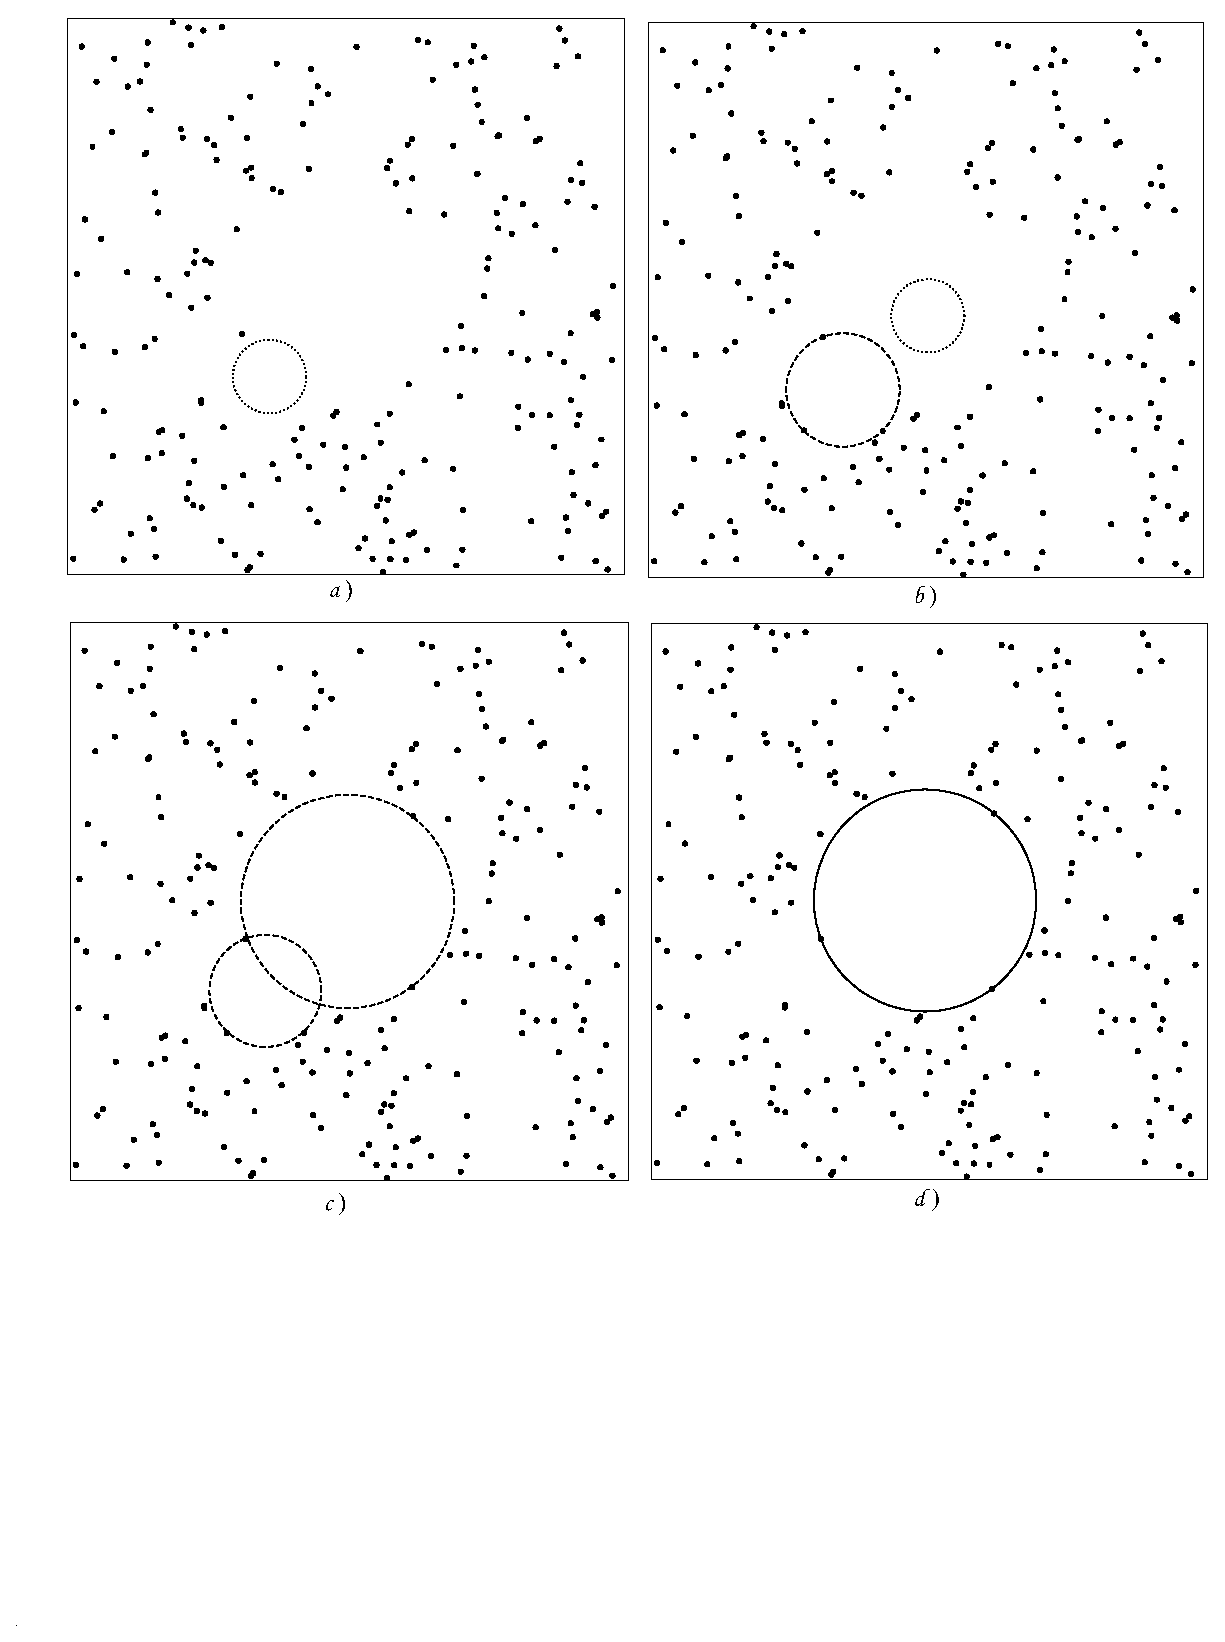
\includegraphics[width=.9\textwidth]{hb.eps}
\caption{HB Void Finder的工作流程:$a)$ 将半径为$R_{\rm min}$的球随即放在样本空间内;
$b)$ 如果随即放置的球为空心,则寻找距离球心最近的四个样本并计算新的中心和半径,并检查其他随机放置的球是否空心;$c)$ 对所有随机放置的空心球重复上一步,最终得到所有新的空心球;$d)$ 新的空心球中如果两个球互相重叠,则将较小的移除,直到只留下不互相重叠的最大的空心球。(文献 ~\inlinecite{Patiri2006HB} 中Figure A2)}
\label{fig:hb}
\end{figure}

\subsection{用巨洞的数密度限制$\sigma_8$和$h\, \Omega_m$的理论模型}


\section{Explicit computation of $P_{\lowercase{n}}(\lowercase{r})$}

%\appendix{Appendix A}\\
%\renewcommand{\theequation}{A-\arabic{equation}}
In this section we show the detailed procedure for computing $P_n(r)$ and the void statistics for given values of $\sigma_8$ and $\Gamma$.

\begin{equation}
P_n(r) = \frac{1}{n!} \int_{-7}^{0} P(\delta_l,r) [u(\delta_l)]^n e^{[-u(\delta_l)]} d\delta_l   \label{eq:eqA1}
\end{equation}

\begin{equation}
u(\delta_l) = \bar{n} V [1+{\rm DELF}(\delta_l,r)] A e^{-b\delta_l^2}    \label{eq:eqA2}
\end{equation}
${\rm DELF}$ is a function of $\delta_l$ and $r$ that gives the mean actual density contrast within a sphere with radius $r$ with enclosed 
linear density contrast $\delta_l$.

\begin{eqnarray}
{\rm DELF}(\delta_l,r) \equiv & \nonumber\\
 \frac{1+{\rm DELT}(\delta_l)}{| 1 - \frac{4}{21}[1+{\rm DELT}(\delta_l)]^{2/3}[\sigma(r[1+{\rm DELT}(\delta_l)]^{1/3})]^{2} |} &    \label{eq:eqA3}
\end{eqnarray}
where ${\rm DELT}(\delta_l)$ denotes the relationship between the actual and linear enclosed density contrasts in the spherical colapse model 
(see PBP06 for details).

\begin{equation}
1+{\rm DELT}(\delta_l) \simeq (1-0.607\delta_l)^{-1.66}   \label{eq:eqA4}
\end{equation}
$\sigma(Q)$ is the rms of the linear density contrast on a sphere with Lagrangian radius $Q$. In this equation, $\sigma(Q)$ is evaluated 
at $Q$ equal to $r[1+{\rm DELT}(\delta_l)]^{1/3}$. Explicit equations for $\sigma$ are given at the end of this Appendix.
$A$, $b$ in eq. (A2) are also functions of $\delta_l$ given by:

\begin{eqnarray}
 A \equiv &A(m,Q=r[1+{\rm DELT}(\delta_l)]^{1/3})  \times  \\
 &\times \left(\frac{D(z)\sigma_8}{0.9}\right)^{0.88} \left(\frac{\Gamma}{0.21}\right)^{0.343} \nonumber \\
 \nonumber\\
 b \equiv &b(m,Q=r[1+{\rm DELT}(\delta_l)]^{1/3})  \times   \\
 & \times \left(\frac{D(z)\sigma_8}{0.9}\right)^{-2.55} \left(\frac{\Gamma}{0.21}\right)^{-0.82} \nonumber \label{eq:eqA5}
\end{eqnarray} 
\\
where $A(m,Q)$, $b(m,Q)$ are functions of the mass of the objects and the Lagrangian radius of the regions being considered (that 
corresponding to an Eulerian sphere with radius $r$, see Rubi\~no et al. 2008):

\begin{eqnarray}
A(m,Q) = &[1.577 - 0.298 (\frac{Q}{8})] - \\
- &[0.0557 + 0.0447 (\frac{Q}{8})] {\rm ln}(m) -\nonumber\\
- &[0.00565 + 0.0018(\frac{Q}{8}][{\rm ln}(m)]^2\nonumber\\
\nonumber\\
b(m,Q) = &[0.0025 - 0.00146 (\frac{Q}{8})] + \\
+ &[0.121 - 0.0156(\frac{Q}{8})] \times \nonumber \\
\times & m^{[0.335 + 0.019 (\frac{Q}{8})]} \nonumber\\
\nonumber\\
m \equiv &\frac{M}{3.51 \times 10^{11} h^{-1}M_{\odot}}\left(\frac{0.21}{\Gamma}\right)    \label{eq:eqA6}
\end{eqnarray}
where $M$ is the mass of the objects, $D(z)$ in equations A5,A6 is the linear growth factor normalized to be 1 at present. The exponents determining the dependence on $A$, $b$ on $\sigma_8$ and redshift are slightly different from those given by Rubi\~no et al. (2008) but are within the precision afforded by the procedure used in that work. The exponents given here have been accurately fitted using numerical simulations. 

For dark matter halos, the values of $m$ entering in these last equations is defined by:
\begin{equation}
\bar{n}(>m)=\bar{n}_{sample}
\end{equation}
while for galaxies we have to use $m_g$ given in equation (\ref{eq:eq14}). The definition of $m$ and $m_g$ imply that these 
quantities have to be scaled with $\sigma_{8}$, $\Gamma$ and redshift. However, $m$ changes very little with these variables up to $z\sim 1$, so we 
chose to held it fixed. In the case of $m_g$ the scaling can be approximated by:

\begin{equation}
m_{g}(\sigma_{8},\Gamma,z) = m (1.124)^{(D(z)\sigma_{8}/0.9)(\Gamma/0.21)^{0.271})}
\end{equation}
 

We use for the probability distribution $P(\delta_l,r)$ of the linear density contrast within an Eulerian space given by Betancort-Rijo \& L\'opez-Corredoira (2002):

\begin{eqnarray}
P(\delta_l,r) = &\frac{exp\left[\frac{-1}{2} \frac{\delta_l^2}{(\sigma(r[1+{\rm DELF}(\delta_l,r)]^{1/3})^2}\right]}{\sqrt{2\pi}} \times \nonumber\\ 
\times &[1 + {\rm DELF}(\delta_l,r)]^{-(1-\frac{\alpha}{2})} \times \nonumber\\
\times &\frac{d}{d\delta_l} \left( \frac{\delta_l}{\sigma(r[1+{\rm DELF}(\delta_l,r)]^{1/3})}\right)\nonumber\\
\alpha(\delta_l,r) = &0.54 + 0.173  \times  ln \left( \frac{r[1+{\rm DELT}(\delta_l)]^{1/3}}{10} \right)    \label{eq:eqA7}
\end{eqnarray}

Even though $\alpha$ depends on $\Gamma$, and the above equation corresponds to $\Gamma=0.21$, this dependence is not relevant for our purposes.

To obtain $\sigma(Q)$ we use the standard BBKS power spectrum (Bardeen et al. 1986). We also checked other power spectra (e.g. Einseinstein \& Hu 1999), finding no significant differences in the final results, i.e.

\begin{eqnarray}
\sigma(Q) \equiv \sigma(Q,\Gamma) \simeq \sigma_8 A(\Gamma) Q^{(-B(\Gamma)-C(\Gamma)\ln{(Q)})} \nonumber\\
A(\Gamma) \equiv 2.01 + 3.9 \Gamma ; B(\Gamma) \equiv 0.2206 + 0.361 \Gamma^{1.5} \nonumber \\
C(\Gamma) \equiv 0.182 + 0.0411 \ln{(\Gamma)}     \label{eq:eqA8}
\end{eqnarray}

This fit is valid for $Q\geq 3 h^{-1}$Mpc and $0.1 \geq \Gamma \geq 0.5$.

To obtain $P^{\star}_n(r^{\star})$, i.e. the probability that a sphere of radius $r^{\star}$ in redshit space contains $n$ objects when placed at random within the distribution, we have to implement the replacements given in equations (16) and (17) in all expressions entering in eq. (A1) but for computational reasons we choose to follow an equivalent procedure whereby $r$ is replaced by:

\begin{equation}
r^{\star} \left( \frac{[1-{\rm VEL}(\delta)]^4 - 1}{-4 {\rm VEL}(\delta)}\right)^{1/3}    \label{eq:eqA9}
\end{equation}
where the function ${\rm VEL}(\delta)$ is defined so that the peculiar velocity, $V$, of mass element at distance $r$ from the center of a spherical mass concentration (or defect) enclosing actual density contrast $\delta$ is given by: 
\begin{equation}
V = H~r~ {\rm VEL}(\delta)   \label{eq:eqA10}  
\end{equation}
where $H$ is the Hubble constant at the time being considered.
Betancort-Rijo et al. (2006) showed that:

To obtain $P_n(r)$ in redsift space, that we represent by $P^{\star}_{n}(r^{\star})$, within this approximation, we may use equation (\ref{eq:eq10}) with the following replacement:  

\begin{equation} 
[1+\delta(\delta_{l},r)] \rightarrow [1+\delta(\delta_{l},r)][1+{\rm VEL}(\delta_{l})]^{-1}  \label{eq:eq20} 
\end{equation}  
\\  

\begin{equation}
{\rm VEL}(\delta) = -\frac{1}{3} \frac{d~ln D(a)}{d~ln a} \frac{{\rm DELK}(\delta)}{1+\delta} \left( \frac{d}{d\delta} {\rm DELK}(\delta) \right)^{-1}   \label{eq:eqA11}
\end{equation}
$D(a)$ is the growth factor as a function of the expansion factor, $a$, and ${\rm DELK}(\delta)$ is the inverse function of ${\rm DELT}(\delta_l)$ 
(see Sheth \& Thormen 2002):

\begin{eqnarray}
{\rm DELK}(\delta) = \frac{\delta_c}{1.68647} ( 1.68647 - \frac{1.35}{(1+\delta)^{2/3}} - \nonumber \\
- \frac{1.12431}{(1+\delta)^{1/2}} + \frac{0.78785}{(1+\delta)^{0.58661}} )    \label{eq:eqA12}
\end{eqnarray}
$\delta_c$ is the linear density contrat for spherical collapse model, which for the concordance cosmology at present is 1.676. 
The logarithmic derivative of $D(a)$ is, for a given cosmology, a function of redshift. We can approximate it as:
\begin{equation}
\frac{d {\rm ln}D(a)}{d {\rm ln} a} \simeq 0.47 \left(\frac{(1+z)^{3}}{\Omega_{m}[(1+z)^{3}+\Omega_{\lambda}/\Omega_{m}]} \right)^{0.6}
\end{equation}

  
It must be noted that, although $r$ has to be replaced by eq. A2 in all its appearances in eq. \ref{eq:eqA9}, for computational reasons we only implement 
that replacement on $P(\delta_l,r)$ and in the explicit appearance of $r$ in eq. \ref{eq:eqA2}.

In PBP06 we argued that most of the information carried by void statistics, concerning cosmological parameters, comes from rare voids.
However, as we will see below, more common voids are still relevant to increase the statistics, which is fundamental to constrain cosmological parameters reliably. 
In order to take into account more common voids, the analytical relationships mentioned above have to be improved.

In PBP06 we showed that the VPF [that we denote here as $P_{0}(r)$] is related to the number density of voids larger 
than a radius $r$ [$\bar{n}_{v}(r)$] by the following expression (for the rare voids limit):

\begin{equation}
\bar{n}_{v}(r) \simeq \frac{3\pi^2}{32}\frac{(\bar{n}'V)^3}{V}P_{0}(r) \label{eq:eq1}
\end{equation}
where
\begin{equation}
\bar{n}'V=-\frac{1}{3}\frac{d\ln P_{0}(r)}{d\ln r} ;\qquad V=\frac{4}{3}\pi r^3   \label{eq:eq2} %\nonumber
\end{equation}
and $\bar{n}'V$ is the mean density of points in the surface of a randomly chosen empty sphere with radius $r$, that we denote in term of 
the derivative of $P_{0}(r)$ with respect to $r$.

Equation (\ref{eq:eq1}) gives an unique functional relationship between $P_{0}(r)$ and $\bar{n}_{v}(r)$. As mentioned above, this works well for 
rare voids, but for more common voids the existence of a unique functional relationship has to be studied. Note that the VPF is determined by all the 
hierarchy of correlations functions (White 1979), but the VPF itself do not determine uniquely all these correlations. For instance, two samples could have 
the same VPF and still differ in some aspect of the clustering, which will render different number densities of voids larger than a given radius.
To address this issue we carried out a detailed analysis using the Millennium Run numerical simulation (Springel et al. 2005; see section \ref{res}). We found evidence for an unique 
functional form of the VPF for the distributions relevant to this work. We write this expression as an extension of the relationship given in equation (\ref{eq:eq1}), i.e.

\begin{equation}
\bar{n}_{v}(r) \simeq \frac{0.68K(r)}{V} e^{-3.5K(r)[1-2.18K(r)]} \label{eq:eq3}
\end{equation}
and
\begin{equation}
K(r)=\bigg(-\frac{1}{3}\frac{d\ln P_{0}(r)}{d\ln r}\bigg)^3 P_{0}(r) \quad;\quad V=\frac{4}{3}\pi r^3 \label{eq:eq4}
\end{equation}
These equations are valid for $K(r) \leq 0.46$, while for $K(r)> 0.46$ $\bar{n}_{v}(r)=0.313/V$. The quantity $K(r)$ measures the rareness of the voids. 
In the rare void limit $K(r)$ goes to zero, so the exponential factor is close to one, recovering the original equation (\ref{eq:eq1}). Note also that 
the coefficient $3\pi^2/32$ shown in equation (\ref{eq:eq1}) is replaced by 0.68 in equation (\ref{eq:eq3}). The former coefficient was originally introduced 
by Preskill \& Politzer (1986), but we found the latter to be more accurate (Betancort-Rijo, in preparation). 

\section{Mass Function}
The unconditional mass function of collapsed objects. $n_{u}(m)$ is given with high accuracy 
by the unconditional Sheth \& Tormen approximation (Sheth \& Tormen 1999, 2002; hereafter ST):

\begin{eqnarray}
    n_{\rm uST}(m,\delta_{c},\sigma(m)) &=& - \left( \frac{2}{\pi} \right)^{1/2}
    A \left[ 1 + \left( \frac{a \delta_{\rm c}^2}{\sigma^2} \right)^{-p}
    \right]  \label{eq:eq10} \\
    & \times& a^{1/2} \frac{\varrho_{\rm b}}{m}
    \frac{\delta_{\rm c}}{\sigma^2} \frac{{\rm d} \sigma}{{\rm d} m}
    \exp \left( - \frac{a \delta_{\rm c}^2}{2 \sigma^2} \right)   \nonumber
\end{eqnarray}
where $A=0.322$, $p=0.3$ and $a=0.707$, $\varrho_b$ stands for the background density,
$\sigma$ is the $rms$ linear mass density fluctuation and $\delta_c$ is the value of 
$\delta_l$ corresponding to collapse in the spherical model which for the cosmological 
parameters that we use ($\Omega_m$=0.3, $\Omega_\lambda$=0.7) is 1.676.
Our problem now is to obtain a similarly accurate approximation to the
conditional mass function, $n_{c}(m,q,Q,\delta_{l})$, so that we can use it in Eq.(\ref{eq:eq999}).

\section{Correlation Function}

Formalism for void two point correlation function is:
\begin{equation} \label{xi_r}
\xi(r) = -1 \times (1-P(r))+P(r)\times[F(r,\delta_L)-1]
\end{equation}

P(r) is the probability that two randomly chosen voids with radius larger than r have a sum of their radius, $R_1$, $R_2$, smaller than r(i.e. $ R_1 + R_2 \le r $). So expression simply says that with probability 1-P(r) (i.e. the probability that $R_1 + R_2  > r$) the CF is -1 and with probability P(r) the CF is certain function of r and $\delta_L$. 

For $F(r,\delta_L)$ we have:
\begin{eqnarray}
F(r,\delta_L) = \frac{\mathrm{ercf}\left(\frac{\delta_L A(r)} {\sqrt{2}B(r)}\right)} {\mathrm{ercf}\left(\frac{\delta_L} {\sqrt{2} \sigma(Q)}\right)} \\
A(r) \equiv 1- \frac{\sigma_{12}(Q,r)} {(\sigma(Q))^2} \\
B(r) = \sigma(Q) \times \left( 1 - \frac{\sigma_{12}^{2}(Q,r)} {\sigma^{4}(Q)}  \right)^{1/2} \\
Q \equiv R_{min}(1+\delta)^{1/3} \\
\delta = DELT(\delta_L)
\end{eqnarray}
where $R_{min}$ is the lower limit for the radius of the voids under consideration. The quantity $\delta_L$ is the linear value of the density fluctuation that correspond to an actual value $\delta$ in spherical framework.

From "On an Analitical..." (Patiri et al 2006),
\begin{eqnarray}
\delta = D(\delta _L) \equiv 0.993[(1-0.607(\delta _{L}-6.5\times 10^{-3} \times \nonumber \\ 
\times (1-\theta(\delta_{L})+\theta(\delta_{L}-1.55))\delta_L^2))^{-1.66}-1]\nonumber  \label{eq:eq4}
\\
\end{eqnarray}
Note that A, B, $\sigma$ are in fact functions of r and $\delta_L$.
\begin{eqnarray}
\sigma^{2}(Q)  = \frac{1}{2\pi^2} \int^{\infty}_{0} P(k) W^2(Qk) k^2 \mathrm{d}k \\
\sigma_{12}(Q,r) = \frac{1}{2\pi^2} \int^{\infty}_{0} P(k) W^2(Qk) \frac{\sin{(kr)}} {r} k \mathrm{d}k
\end{eqnarray}


\begin{eqnarray}\label{PK}
P(k) =&  \sigma_8^2 \times 1.9843\times 10^4 \times \log{(1.0+11.14\times k)}^2 \times \nonumber\\ 
 &(1 + 1.85\times k + 5580.0\times k^2 + 17580.0\times k^3 + 1.04\times 10^6 \times k^4)^{-0.5} \times \frac{1}{k}
\end{eqnarray}
where P(k) is the power spectra. W(x) is defined by:
$$
W(x) \equiv \frac{3}{x^3} (\sin{x} - x\cos{x})
$$
The goal is to fit the main part of the CF by following this procedure for different values of $\delta_L$(the values of $\delta_L$ I expect to be between -4 and -6) and looking for the best fit.



\chapter{数据:模拟暗物质晕表、SDSS观测数据及其模拟光锥星系表}
\label{cha:data}

\section{引言}

在使用BOSS/SDSS-III CMASS样本前,需要在很大的空间里用许多组星系表或暗物质晕表研究巨洞的统计性质。我们用基于微扰论的近似方法~\cite{Kitaura2014,Kitaura2015}(The PerturbAtion Theory Catalogue generator of Halo and galaxY,\textsc{PATCHY})生成了100组具有相同宇宙学模型的模拟暗物质晕表(mock catalogues)。这100组模拟暗物质晕表唯一的区别是生成它们各自初始密度场时随机数生成器使用了不同的种子(seeds),其他参数完全一样。这100组模拟暗物质晕表在后文被称作完整的模拟暗物质晕表(Complete halo mock catalogues)。

\textsc{PATCHY}使用BigMultiDark N-body simulations~\cite{Klypin2014}作为基准对参数进行标定,其宇宙学参数与Planck $\Lambda$CDM的宇宙学一致:$\Omega_{\rm M} = 0.307115$、$\Omega_b = 0.048206$、$\sigma_8 = 0.8288$、$n_s = 0.96$,哈勃参量为$H_0 \equiv 100\,h\,\mathrm{km}\,\mathrm{s}^{-1}\mathrm{Mpc}^{-1}$其中$h = 0.6777$。在边长为2.5\,$h^{-1}$ Gpc并具有周期性边界条件的立方体内,\textsc{PATCHY}将空间分为$960^3$个格点,网格的分辨率为2.6\,$h^{-1}$ Mpc,并通过augmented Lagrangian perturbation theory~\cite{Kitaura2013}(ALPT)来计算密度场。\textsc{PATCHY}细致的考虑了欧拉非线性偏袒(Eulerian non-linear bias)和随机偏袒(stochastic bias),并以此生成数密度为 $3.5\times10^{-4}\,h^3\,\mathrm{Mpc}^{-3}$的暗物质晕表。这个数密度与BOSS CMASS LRG样本在平均红移$z \simeq 0.56$处的平均数密度相同。

因为\textsc{PATCHY}是基于微扰论生成的暗物质晕表,这些暗物质晕表相对于用宇宙学大尺度结构N体数值模拟产生的模拟暗物质晕表不够准确,但是在统计性质上(两点和三点统计性质)可以十分接近~\cite{Chuang2015,Zhaocheng2015},在后文中如果不特别强调是由N体数值模拟产生的模拟暗物质晕表,模拟暗物质晕表都是指基于\textsc{PATCHY}生成的模拟暗物质晕表。我们使用这些模拟暗物质晕表研究巨洞的平均2PCF和估算协方差矩阵。

之后使用了BOSS/SDSS-III CMASS样本的DR11
%和DR12两部分
观测数据和相应的1024组与观测数据具有相似空间分布与统计性质的模拟星系表。这些模拟星系表也是用\textsc{PATCHY}生成的,经过Halo Abundance Matching~\cite{Rodriguez-Torres2016}(HAM)将模拟暗物质晕表转换成模拟星系表,把不同红移处的星系模拟星系表拼接起来并使具有光锥一样的几何形状,在后文被称作\textsc{PATCHY}光锥模拟星系表或模拟光锥星系表。本章详细介绍了这几组不同的模拟暗物质晕表、模拟光锥星系表和观测数据。

\section{完整的模拟暗物质晕表}
\label{sec:datacomple}

我们用\textsc{PATCHY}在边长为2.5\,$h^{-1}$Gpc并具有周期性边界条件的立方体内生成了100组模拟暗物质晕表。这100组完整的模拟暗物质晕表具有相同宇宙学模型,唯一的区别是生成各自初始密度场时随机数生成器使用了不同的种子。这些模拟暗物质晕表记录了暗物质晕在共动距离($h^{-1}$ Mpc)下的位置坐标($x_1$,$x_2$,$x_3$)和对应方向的速度($v_1$,$v_2$,$v_3$),数密度为$3.5\times10^{-4}\,h^3\,\mathrm{Mpc}^{-3}$,且所有暗物质晕都在红移$z = 0.5618$处。这些模拟暗物质晕表内记录的位置是暗物质晕在空间的真实位置,所以这部分数据被称为实空间模拟暗物质晕表(real space mock halo catalogues)。

假设观测者在$x_3$方向的无穷远处观测实空间完整模拟暗物质晕表内所记录的暗物质晕的红移和方向,暗物质晕的在$x_3$方向的本动速度会使其被观测到的红移发生变化,从而使其位置相对真实位置也发生一定程度的偏移。
这个因本动速度影响而使被观测天体位置相对真实位置发生偏移的现象叫做红移畸变效应(redshift space distortion,RSD)。
考虑RSD效应的完整模拟暗物质晕表的位置信息,与在无穷远处的观测者通过观测到的红移而转换成的位置信息相同,因此考虑RSD效应的完整模拟暗物质晕表被称作红移空间模拟暗物质晕表(redshift space mock halo catalogues)。

\begin{figure}
\centering
\includegraphics[width=.9\textwidth]{pk_ratio}
\caption{\textsc{PATCHY}所使用的两个初始物质功率谱,绿色实线是用Planck $\Lambda$CDM的宇宙学通过CAMB计算得到的有声学振荡的物质密度功率(wiggle),对绿色实线做平滑得到蓝色实线,也就是没有声学振荡的物质密度功率谱(nonwiggle)。上图画出来两个功率谱的形状,为了更清晰的表现两者的形状图中画的是$k P_{auto}$,下图展示了两个功率谱的比值。}
\label{fig:pkratio}
\end{figure}

\section{无BAO的完整的模拟暗物质晕表}
\label{sec:datanw}

用\textsc{PATCHY}在边长为2.5\,$h^{-1}$Gpc并具有周期性边界条件的立方体内生成了100组模拟暗物质晕表,生成这些模拟暗物质晕表的初始密度场的功率谱中没有声学振荡的成分,其他条件与实空间的100组完整模拟暗物质晕表完全相同。图~\ref{fig:pkratio} 展示了这些没有声学振荡的初始密度功率谱与前面实空间完整模拟暗物质晕表的初始密度功率谱。因为声学振荡在初始密度功率谱的特征就是图~\ref{fig:pkratio} 中下半部分所示的一系列振荡,通过对有声学振荡初始密度功率谱做平滑可以得到没有声学振荡的初始密度功率谱。

\section{\textsc{PATCHY}光锥模拟星系表}
\label{sec:lightcone}

利用观测数据能得到一个测量结果,有两大类方法可以去估算测量结果的误差。一种是将整个巡天分成几份,把每一份当成一个独立的观测,然后通过刀切法复采样(jackknife resampling)或自举复采样(bootstrap resampling)来估算误差。这种方法虽然曾经被使用过~\cite{Norberg2009},但是并不能很好的考虑系统误差的影响,不容易帮助人们研究结果背后的物理。另外体积变小后,对于比子样本体积更大的尺度上的误差估算会非常不可靠,这一点对于研究BAO尤为致命。另一种方法是用许多组宇宙大尺度结构数值模拟的数据来估算观测结果的误差,这种方法估算的误差更加可靠。使用N体数值模拟可以非常精确的再现宇宙大尺度结构,但是这种方式需要非常大的计算量,不可能批量生成上千组结果。而\textsc{PATCHY}可以比较精确的再现宇宙大尺度结构,其两点、三点统计性质与N体数值模拟的结果相差非常小,同时其对计算量的需求远远小于N体数值模拟。所以BOSS最后两次发布的数据都采用了\textsc{PATCHY}生成的光锥模拟星系表来估算观测结果的误差。

生成可靠的\textsc{PATCHY}光锥模拟星系表以估算观测结果的误差需要进行以下几步处理:
\begin{description}
\item[1.] 使用N体数值模拟(BigMultiDark Simulations~\cite{Klypin2014})在一系列不同红移处,生成可以精确呈现暗物质晕内部子结构的暗物质晕表。在不同的红移处,选用适当的参数通过HAM把模拟暗物质晕表转化成模拟星系表~\cite{Rodriguez-Torres2016}。
\item[2.] 在不同红移处,分别调整\textsc{PATCHY}的参数,使其生成的暗物质晕模拟暗物质晕表与所在红移处的模拟星系表具有相同的两点和三点成团性。
\item[3.] 用HADRON~\cite{Zhaocheng2015}(Halo mAss Distribution ReconstructiON)计算\textsc{PATCHY}生成的每一个暗物质晕的恒星质量。
\item[4.] 用SUGAR~\cite{Rodriguez-Torres2016}(The SUrvey GenerAtoR)将不同红移处的\textsc{PATCHY}模拟星系表拼接成光锥模拟星系表,并使其与观测数据具有一样的几何形状、巡天区域和选择效应,并在整个空间与观测数据具有相同的数密度分布。
\end{description}

BOSS DR11一共有1024个\textsc{PATCHY}光锥模拟星系表,BOSS DR12有2048个\textsc{PATCHY}光锥模拟星系表,这些数据被用于后续的相应研究。图~\ref{fig:pie} 展示了在Southern Galactic Cap(SGC)和Northern Galactic Cap(NGC),\textsc{PATCHY}光锥模拟星系表很好的再现了BOSS DR12在空间的分布。

\begin{figure}
\includegraphics[width=15.cm]{pie}
\put(-380,390){\rotatebox[]{0}{BOSS DR12}}
\put(-125,45){\rotatebox[]{0}{MULTIDARK}}
\put(-125,30){\rotatebox[]{0}{PATCHY MOCKS DR12}}
\put(-20,210){\rotatebox[]{-90}{180$^{\rm o}$}}
\put(-417,210){\rotatebox[]{90}{180$^{\rm o}$}}
\put(-10,210){\rotatebox[]{-90}{\text{Northern Galactic Cap}}}
\put(-427,210){\rotatebox[]{90}{\text{Northern Galactic Cap}}}
\put(-40,290){\rotatebox[]{-90}{210$^{\rm o}$}}
\put(-397,290){\rotatebox[]{90}{150$^{\rm o}$}}
\put(-100,350){\rotatebox[]{-90}{240$^{\rm o}$}}
\put(-337,350){\rotatebox[]{90}{120$^{\rm o}$}}
\put(-40,130){\rotatebox[]{-90}{150$^{\rm o}$}}
\put(-397,130){\rotatebox[]{90}{210$^{\rm o}$}}
\put(-100,70){\rotatebox[]{-90}{120$^{\rm o}$}}
\put(-337,70){\rotatebox[]{90}{240$^{\rm o}$}}
\put(-145,380){\rotatebox[]{0}{330$^{\rm o}$}}
\put(-297,380){\rotatebox[]{0}{30$^{\rm o}$}}
\put(-145,40){\rotatebox[]{0}{30$^{\rm o}$}}
\put(-297,40){\rotatebox[]{0}{330$^{\rm o}$}}
\put(-255,410){\rotatebox[]{0}{\text{Southern Galactic Cap}}}
\put(-220,400){\rotatebox[]{0}{0$^{\rm o}$}}
\put(-220,23){\rotatebox[]{0}{0$^{\rm o}$}}
\put(-255,13){\rotatebox[]{0}{\text{Southern Galactic Cap}}}
\put(-192,280){\rotatebox[]{0}{2.7}}
\put(-252,280){\rotatebox[]{0}{0.2}}
\put(-172,315){\rotatebox[]{0}{5.1}}
\put(-272,315){\rotatebox[]{0}{0.4}}
\put(-152,350){\rotatebox[]{0}{7.3}}
\put(-292,350){\rotatebox[]{0}{0.6}}
%
\put(-195,300){\rotatebox[]{60}{\text{lookback time in billions of years}}}
%
\put(-280,300){\rotatebox[]{-60}{\text{redshift}}}
%
\put(-260,233){\rotatebox[]{-58}{\Huge$\leftharpoondown$}} %longleftarrow$}}
\put(-190,183){\rotatebox[]{-238}{\Huge$\leftharpoondown$}} %longleftarrow$}}
\put(-275,220){\rotatebox[]{0}{\text{OBSERVATIONS}}}
\put(-225,200){\rotatebox[]{0}{\text{THEORY/MODEL}}}
\put(-192,145){\rotatebox[]{0}{2.7}}
\put(-252,145){\rotatebox[]{0}{0.2}}
\put(-172,110){\rotatebox[]{0}{5.1}}
\put(-272,110){\rotatebox[]{0}{0.4}}
\put(-152,75){\rotatebox[]{0}{7.3}}
\put(-292,75){\rotatebox[]{0}{0.6}}
\put(-73,410){\rotatebox[]{0}{\text{log M$_*$}}}
\put(-115,388){\rotatebox[]{0}{\tiny\text{10.9}}}
\put(-90,388){\rotatebox[]{0}{\tiny\text{11.1}}}
\put(-67,388){\rotatebox[]{0}{\tiny\text{11.3}}}
\put(-43,388){\rotatebox[]{0}{\tiny\text{11.5}}}
\put(-20,388){\rotatebox[]{0}{\tiny\text{12.0$<$}}}
\caption{ BOSS DR12 观测数据(左上部分)和\textsc{PATCHY光锥模拟星系表}(\textsc{MULTIDARK PATCHY MOCKS DR12},右下部分)在空间中的分布。(文献 ~\inlinecite{Kitaura2016}中的Figure 2)}
\label{fig:pie}
\end{figure}

\begin{figure}
\centering
\includegraphics[width=.9\textwidth]{Anderson2014_figure1_dNdzhist}
\caption{BOSS/SDSS DR11 样本中LOWZ(红色)和CMASS(绿色)的星系数密度随红移的分布。蓝色柱状图是SDSS-II DR7的星系数密度随红移的分布~\cite{Abazajian2009DR7}。(文献 ~\inlinecite{Anderson2014441} 中的Figure 1)}
\label{fig:AndersonFig1}
\end{figure}

\section{BOSS/SDSS-III CMASS DR11星系表}

BOSS~\cite{Eisenstein:2011sa, Bolton:2012hz, Dawson2013}是SDSS-III的重要组成部分,观测使用的是位于新墨西哥州(New Mexico)的阿帕奇天文台(Apache Point Observatory)的2.5米斯隆望远镜(Sloan Telescope)~\cite{Gunn2006}。BOSS使用了相比SDSS I/II升级后的光谱仪,可以得到波长范围3600-10000\r{A}内分辨率为1500-2600\r{A}的光谱~\cite{Smee2013}。计划在10000平方度的天区内,LOWZ和CMASS两个红移区间,获得135万个星系的光谱和红移(图~\ref{fig:AndersonFig1})。这些星系是通过SDSS DR8~\cite{Aihara2011}的图像观测筛选出来的LRG。我们的工作中只使用了CMASS样本。从SDSS DR8中筛选CMASS目标LRG的条件为
\begin{eqnarray}
 17.5 < i_{\rm cmod}  < 19.9\\
r_{\rm mod} - i_{\rm mod}  < 2 \\
d_{\perp} > 0.55 \label{eq:hcut}\\
i_{\rm fib2} < 21.5\\
i_{\rm cmod}  < 19.86 + 1.6(d_{\perp} - 0.8) \label{eq:slide}
\end{eqnarray}
其中$i$和$r$是相应波段的星等,$i_{\rm fib2}$是$i$波段在2角秒孔径的星等,下标“mod”指$r$波段德沃古勒(DeVaucouleurs)和指数轮廓(exponential profile)的最佳拟合值~\cite{Stoughton2002},下标“cmod”指段德沃古勒和指数轮廓线性组合的最佳拟合值~\cite{Abazajian2004},$d_{\perp}$定义为
\begin{equation}
d_{\perp} = r_{\rm mod} - i_{\rm mod} - (g_{\rm mod} - r_{\rm mod})/8.0
\label{eq:dp}
\end{equation}
将星系与恒星区分开的条件是
\begin{eqnarray}
i_{\rm psf} - i_{\rm mod} > 0.2 + 0.2(20.0-i_{\rm mod})  \label{eq:sgsep1}\\
z_{\rm psf}-z_{\rm mod} > 9.125 -0.46\,z_{\rm mod} \label{eq:sgsep2},
\end{eqnarray}
其中下标“psf”指点扩散函数(point spread function)。

CMASS的星系分布在红移$0.43 < z < 0.7$的范围内,星系数密度在 $z \approx 0.5$达到峰值(图~\ref{fig:AndersonFig1})。对于BOSS CMASS DR11观测数据和光锥模拟星系表的研究,我们只使用了红移$0.45 < z < 0.65$内的数据。图~\ref{fig:footprints}展示了DR11所覆盖的天区。

BOSS的样本中存在一些系统性偏差,比如有些星系不能测量红移(redshift failure),或者因为获取星系光谱时,相邻两根光纤的最近距离不能小于$55^{\prime\prime}$从而造成一些星系无法被观测到(fiber collision)。而星系成团性分析的结果会严重受到这些问题影响。通过文献 ~\inlinecite{Ross2012}中提出的方法,给每个星系不同的权重可以在一定程度上减小系统性偏差对星系成团性的影响~\cite{Ross2012,Chuang2016}。每个星系的权重是
\begin{equation}
w_g = w_{star} w_{see} (w_{zf} + w_{cp} - 1)
\label{EQ:weight}
\end{equation}
其中$w_{zf}$是测量红移失败的权重,$w_{cp}$是两个星系离的很近的权重(the close pair weight),$w_{star}$是用来处理星系数密度与恒星数密度系统性关系的权重,$w_{see}$是修正视宁度(seeing)的权重。$w_{zf}$和$w_{cp}$对CMASS样本的影响很小~\cite{Ross2012},所以在光锥模拟星系表中没有考虑这两个权重所对应的效应。DR11 CMASS样本使用这个方法计算出了每个星系的权重~\cite{Anderson2014441},计算观测星系2PCF时使用了这些权重。图~\ref{fig:CMASSpkxi}中是BOSS CMASS DR11观测样本星系的2PCF和功率谱。

\begin{figure}
\centering
\resizebox{\textwidth}{!}{\includegraphics{BOSS_CMASS_footprint_comparison1}}
\caption{ 从BOSS DR9到DR11巡天观测所覆盖的天区。上半部分是NGC方向的结果,下半部分是SGC方向的结果。不同颜色表示了光谱测量的完成度。灰色区域是BOSS计划观测但是尚未观测的天区。DR9、DR10和DR11所覆盖的天区面积分别为3275、6161和8377平方度。(文献 ~\inlinecite{Anderson2014441} 中的Figure 2)}
\label{fig:footprints}
\end{figure}

\begin{figure}
\centering
\resizebox{0.8\textwidth}{!}{\includegraphics{aard2pt4pan_CMASS.pdf}}
\caption{DR11 CMASS 样本的2PCF$\xi(s)$(左半部分),和功率谱$P(k)$(右半部分)。上半部分是没有经过BAO信号重构的结果,下半部分是经过BAO信号重构的结果。实线是每个情况的最佳拟合。BAO信号重构之后的$\xi(s)$和$P(k)$中,BAO信号的显著性都得到增强。(文献 ~\inlinecite{Anderson2014441} 中的Figure 11)}
\label{fig:CMASSpkxi}
\end{figure}

%\section{BOSS/SDSS-III CMASS DR12星系表}
\chapter{寻找巨洞及巨洞的统计性质}
\label{cha:DIVE}

\section{引言}

德劳内三角剖分~\cite{Delaunay1934}(Delaunay Triangulation,DT)被广泛用于天文学研究中~\cite{Bernardeau1996,Marinoni2002,Pal2006,Cardiel2001,Weygaert2011,Berge2012,Cedres2012}。文献 ~\inlinecite{Schaap2000} 开发了可以利用离散的样本重构连续密度场的Delaunay tessellation field estimator(DTFE),在此基础之上从理论和观测上研究宇宙大尺度结构~\cite{Aragon-Calvo2007,Romano-Diaz2007,Weygaert2009,Platen2011,Sousbie2011,Jennings2012}。文献 ~\inlinecite{Platen2007} 在DTFE的基础上开发了The Watershed Void Finder(WVF),文献 ~\inlinecite{Neyrinck2008}基于Voronoi Diagram开发了ZOBOV,文献 ~\inlinecite{Sutter2015VIDE}对ZOBOV的功能做了一些扩展和强化开发出VIDE。文献 ~\inlinecite{Gaite2005}和文献 ~\inlinecite{Way2015}直接将DT所得到的空心四面体定义为巨洞。

我们把巨洞定义为通过星系分布找到的空心四面体所确定的空心球,并通过DIVE ~\cite{Zhao2016DIVE}对三维空间中星系的分布做DT得到空心四面体,再计算其对应空心球的中心位置和半径,因而这些空心球被称为DT巨洞。DIVE可以非常高效的从离散分布的天体中寻找所有的空心球,因此我们能够将DIVE用于100组实空间和红移空间完整模拟暗物质晕表,并分析巨洞的统计性质。在没有特别声明使用的是红移空间完整模拟暗物质晕表的情况下,都默认是实空间完整模拟暗物质晕表。

根据巨洞的统计性质可以将DT巨洞分为两类。一类相当于星系群,对应\textit{voids-in-clouds}~\cite{SW04}类巨洞,通常半径比较小,中心在高密度区域。另一类是真正宇宙学意义上的巨洞,半径比较大,占据了宇宙中低密度区域,其中的物质朝远离巨洞中心的方向运动,对应\textit{voids-in-voids}~\cite{SW04}类巨洞。

DT巨洞可以互相重叠,而文献 ~\inlinecite{Patiri2006372,VBT12,CC13}中所定义的巨洞不能互相重叠,从DT巨洞中同样可以选出不互相重叠的巨洞子样本(disjoint voids,disjoint巨洞)。本章也比较了DT巨洞和disjoint巨洞之间的差异。

通过计算DT巨洞的潮汐张量(tidal field tensor)能从动力学角度将所有DT巨洞分为宇宙大尺度结构中的不同成分。研究结果表明半径大的巨洞内部的物质都在朝远离巨洞中心的方向运动,这些巨洞都在不断变大。这一结果也表明了半径大的巨洞在低密度区域。

最后计算了不同大小的DT巨洞的功率谱,并发现两类巨洞的偏袒不同,说明两类巨洞分布在不同的大尺度结构中。

\begin{figure}
\centering
\includegraphics[width=.9\textwidth]{DTVoid_box}
\caption{完整模拟暗物质晕表中部分区域内DT巨洞和暗物质晕的相对空间分布。红色空心圆点是巨洞的中心,阴影区域表示了巨洞半径范围内的体积,DIVE找到的每个空心四面体的顶点是暗物质晕所在的位置由蓝色实心圆点表示,黑色直线表示四面体的边。左图:$12^3\,h^{-3}\mathrm{Mpc}^3$体积内半径$R \leq 4\,h^{-1}$Mpc的DT巨洞。右图:$80^3\,h^{-3}\mathrm{Mpc}^3$体积内半径$R \in [26, 27]\,h^{-1}$Mpc的DT巨洞(文献 ~\inlinecite{Zhao2016DIVE}中的Figure 1)}
\label{fig:visual_all}
\end{figure}

\section{DIVE:Delaunay trIangulation Void findEr}
\label{sec:DIVE}

DIVE可以对在三维空间中离散分布的物体,如暗物质晕或星系,做徳劳内三角剖分得到空心四面体,四面体的顶点是暗物质晕或星系所在的位置。通过四面体四个顶点可以唯一的确定一个空心球,并计算得到空心球的中心和半径。DIVE利用开源的Computational Geometry Algorithms Library\footnote{\url{http://www.cgal.org}} ~\cite{Bronnimann2015, Jamin2015}(\textsc{cgal})实现对空间的徳劳内三角剖分并计算空心球的圆心和半径。图~\ref{fig:visual_all} 展示了完整模拟暗物质晕表中一小块区域内,DT巨洞与暗物质晕在空间中的相对分布。半径较大的DT巨洞分布在空的区域,属于\textit{voids-in-voids},而半径较小的DT巨洞在许多暗物质晕中间,属于对应\textit{voids-in-clouds}。相比\textit{voids-in-voids},\textit{voids-in-clouds}对散射噪声(shot noise)更敏感~\cite{Cai2014}。

\textsc{cgal}自身没有任何参数,所以不依赖具体具体宇宙学模型。观测数据所在的空间十分不规则,但\textsc{cgal}对任意形状空间内离散分布的物体都可以进行DT。同时\textsc{cgal}的效率非常高,所以我们得以将其用于大量的完整模拟暗物质晕表进行统计分析。

\begin{figure}
\centering
\includegraphics[width=.9\textwidth]{DTVoid_nonoverlap}
\caption{完整模拟暗物质晕表的$100^3\,h^{-3}\mathrm{Mpc}^3$部分体积内,半径$R \geq 17\,h^{-1}$Mpc的disjoint巨洞的空间分布。红色空心圆是空间内DT巨洞的球心,虚线表示的方形图~\ref{fig:visual_all} 内的区域,阴影区域是所有disjoint巨洞所占据的体积。(文献 ~\inlinecite{Zhao2016DIVE}中的Figure 2)}
\label{fig:visual_dj}
\end{figure}

使用类似HB void finder~\cite{Patiri2006372}的方法可以从DT巨洞中选出disjoint巨洞。这类巨洞与之前大部分定义的巨洞的方式类似,都不允许巨洞之间互相重叠~\cite{Patiri2006HB,Micheletti02014},因而这类巨洞的数密度会显著小于同样大小的DT巨洞。图~\ref{fig:visual_dj} 展示了一个完整模拟暗物质晕表的一部分空间内的disjoint巨洞的分布,从图中以及与图~\ref{fig:visual_all} 的对比可以看出disjoint巨洞的数密度远小于DT巨洞。

如果认为DT巨洞之间有从属关系,disjoint巨洞可以被认为是独立的巨洞(distinct巨洞、parent巨洞),与distinct巨洞重叠的巨洞是这个distinct巨洞的从属巨洞或子巨洞(subvoids)。文献 ~\inlinecite{SW04}就巨洞的从属关系也进行过研究。图~\ref{fig:subvoid} 展示了不同半径的独立巨洞的子巨洞的数量和大小的分布。可以看出更大的独立巨洞倾向于拥有更多并且更大的子巨洞。在一个较大独立巨洞所在的低密度区域内,可以存在非常多与这个独立巨洞半径大小相当的DT巨洞。同一个低密度区域内大量的DT巨洞使得更大的低密度区域拥有更大的权重。

\begin{figure}
\centering
\includegraphics[width=.9\textwidth]{subvoid}
\caption{不半径独立巨洞的子巨洞的数目和半径大小的分布。上图:半径为$R_{V_P}$的独立巨洞的子巨洞的半径$R_{V_S}$分布(颜色深浅表示数目多少),蓝色实线表示子巨洞的平均半径。下图:半径为$R_{V_P}$的独立巨洞的子巨洞的平均数量$N_{V_S}$(黑色实线),和1$\sigma$误差范围(灰色区域)。结果来自一个\textsc{PATCHY}完整模拟暗物质晕表。(文献 ~\inlinecite{Zhao2016DIVE}中的Figure 7)}
\label{fig:subvoid}
\end{figure}

\section{巨洞的数密度}
\label{sec:voidnumberdensity}

巨洞的数密度是巨洞非常重要的一个性质,它决定了巨洞其他统计性质的统计显著性。同时巨洞的数密度分布也可以直接用于限制宇宙学参数~\cite{Patiri2006HB,JLH13}、研究暗能量模型~\cite{Pisani2015PRD,Sutter2015}或研究不同的引力理论~\cite{Cai2015}。

DT巨洞的一大优势就是拥有较大的数密度,结果在统计上更可靠。但DT巨洞是从空间中离散分布的暗物质晕或星系中通过DIVE获得的,其数密度分布肯定在一定程度上依赖于空间中暗物质晕或星系的数密度。实空间和红移空间完整模拟暗物质晕表的数密度都是$3.5\times10^{-4}\,h^{3}\,\mathrm{Mpc}^{-3}$,这是BOSS CMASS样本的LRG平均数密度,有些红移处的LRG数密度低于这个值。因此,我们将完整模拟暗物质晕表内的暗物质晕随机移除一部分,得到三组数密度更低([2, 2.5, 3] $\times 10^{-4}\,h^3\,\mathrm{Mpc}^{-3}$)的完整模拟暗物质晕表。

研究结果表明,随着完整模拟暗物质晕表内暗物质晕数密度的减少DT巨洞的总数也随之显著减少,但是半径$R > 16$ $h^{-1}$ Mpc的DT巨洞总数几乎保持不变,半径$R > 20$ $h^{-1}$ Mpc的巨洞数量增多,同时半径$R < 10$ $h^{-1}$ Mpc的巨洞数量减少(图~\ref{fig:ndens_nmean} 右半部分)。以此可以将DT巨洞分为两类,一类跟暗物质晕正相关,另一类与暗物质晕反相关,两类巨洞的分界线在$R \sim 16$ $h^{-1}$ Mpc。对于disjoint巨洞来说,这一分界位于$R \sim 17.5$ $h^{-1}$ Mpc,与文献 ~\inlinecite{Hamaus2014}的结果($R \sim 17.6$ $h^{-1}$ Mpc)非常接近。

\begin{figure}
\begin{tabular}{cc}
\includegraphics[width=.47\textwidth]{numdens_nmean}
\includegraphics[width=.47\textwidth]{numdens_nmean_cum}
\end{tabular}
\caption{不同颜色的线表示不同数密度的完整模拟暗物质晕表内,巨洞的数量分布(number function,左图)和累积数数量分布(cumulative number function,右图)。阴影区域为1-$\sigma$误差范围,误差非常小所以看上去像实线。(文献 ~\inlinecite{Zhao2016DIVE}中的Figure 4)}
\label{fig:ndens_nmean}
\end{figure}

\begin{figure}
\centering
\includegraphics[width=.9\textwidth]{numdens_z}
\caption{实空间与红移空间中DT巨洞和disjoint巨洞的数量分布。1-$\sigma$误差范围非常小,肉眼不可分辨。(文献 ~\inlinecite{Zhao2016DIVE}中的Figure 6)}
\label{fig:ndens_z}
\end{figure}

红移空间的DT巨洞与红移空间的暗物质晕或星系存在一些本质上的区别。对于暗物质晕或星系来说,实空间的位置与红移空间的区别是由于本动速度的存在而使得观测的红移与真实的红移不一致造成的。两者的区别只是视线方向上的位置发生了改变。但是通过DIVE获得的DT巨洞只有球心的位置和半径,没有适当的方式可以被用来定义DT巨洞的速度,因而不能通过DT巨洞在视线方向上的本动速度来将其从实空间转换到红移空间。因为暗物质晕或星系的位置发生了改变,即便可以通过一定的方式将DT巨洞从实空间转换到红移空间,其内部也可能会存在暗物质晕或星系,这与我们对巨洞的定义相矛盾。我们的最终目标是将DIVE用于红移空间中因观测效应而存在各种系统偏差的真实观测数据,不可能直接获得宇宙中星系在实空间中的真实位置。为了保持对巨洞的定义不变,只能将DIVE用于红移空间的完整模拟暗物质晕表来获得红移空间的巨洞数据。而巨洞性质在实空间与红移空间的区别是由暗物质晕或星系的RSD效应间接造成的。

从图~\ref{fig:ndens_z} 的结果可以合理推测,半径较大的DT巨洞或disjoint巨洞,其内部和周围的物质都在朝远离巨洞中心的方向运动,所以在红移空间半径较大的巨洞所在的没有暗物质晕或星系的空旷区域会沿视线方向被拉长,从而使得其中巨洞的半径略微变大。所以红移空间中有更多半径较大的巨洞。非线性RSD效应(Fingers-Of-God,FOG)使得中等半径的巨洞数量减少。因为\textsc{PATCHY}的分辨率为$2.6\,h^{-1}$Mpc,所以结果中更小尺度的RSD效应相比真实情况可能存在一些偏差。

\section{巨洞中心在空间中的分布}

在最早的星系巡天中,发现一些较大的区域内星系的数密度远小于理论预期~\cite{KOS81},或者连续的很大空间内没有观测到任何星系~\cite{LGH86,VGP94},从而发现了巨洞的存在。一般认为在宇宙的高密度区域物质塌缩形成暗物质晕和星系,所以没有暗物质晕或星系的地方可以被认为是宇宙中的低密度区域,也就是巨洞所在的地方。本章我们研究了巨洞中心在空间中相对暗物质晕的分布。

图~\ref{fig:densfield} 展示了实空间完整模拟暗物质晕表的同一区域内,物质密度场、暗物质晕和DT巨洞归一化后的数密度在($x$,$y$)方向上的投影。暗物质晕分布在物质密度场中的高密度区域。所有DT巨洞归一化后的数密度分布与物质密度场也符合的较好,这是因为DT巨洞中半径较小的巨洞占大多数(图~\ref{fig:visual_all})。半径$R \geq 16\,h^{-1}$Mpc的巨洞中心分布在物质密度场中的低密度区域,同时从图~\ref{fig:densfield} 中最下面的图中可以看到,这些巨洞的中心分布在没有暗物质晕的空旷区域,两者共同占据了整个空间。这个结果又一次证明半径$R \geq 16\,h^{-1}$Mpc的DT巨洞中心分布在宇宙低密度区域。

\begin{figure}
\centering
\includegraphics[width=.9\textwidth]{densfield}
\caption{一个完整模拟暗物质晕表的$1000\times500\times50\,h^{-3}\mathrm{Mpc}^3$体积内,物质密度场、暗物质晕(halos)、所有DT巨洞(DT Voids)和半径$R \geq 16\,h^{-1}$Mpc的巨洞(\textit{Large} Voids)相对平均数密度归一化后的数密度分布,最下面的图中为了区别于暗物质晕,\textit{Large} Voids的数密度用负数表示。(文献 ~\inlinecite{Zhao2016DIVE}中的Figure 8)}
\label{fig:densfield}
\end{figure}

\section{巨洞附近的物质密度分布}

上一节我们定性的分析了DT巨洞在物质密度场中的分布,这一节我们定量的分析巨洞中心区域的物质密度及巨洞内部和周围的物质密度轮廓(Density profiles)。

\subsection{巨洞中心的物质密度}

通过\textsc{PATCHY}计算物质密度场时将空间分为$960^3$个网格,分辨率为$2.6\,h^{-1}$Mpc。DT巨洞中心处的物质密度反差$\delta_m$(density contrast,$\delta_m \equiv \rho_m / \bar{\rho}_m - 1$)为离中心最近的一个网格的$\delta_m$。图~\ref{fig:radens} 展示了不同半径DT巨洞在不同$\delta_m$处的数量。大半径的DT巨洞中心的$\delta_m$几乎都很小且平均值小于0,而小半径的DT巨洞中心$\delta_m$普遍很大与暗物质晕的$\delta_m$相当。DT巨洞中心的平均$\delta_m$随着半径的增加而减小。

\begin{figure}
\centering
\includegraphics[width=.9\textwidth]{radens}
\caption{不同半径的DT巨洞中心在不同物质密度反差$\delta_m$的数量。蓝色实线表示不同半径DT巨洞中心的平均$\delta_m$,绿色实线是暗物质晕的平均$\delta_m$。(文献 ~\inlinecite{Zhao2016DIVE}中的Figure 9)}
\label{fig:radens}
\end{figure}

\subsection{巨洞的物质密度轮廓}

巨洞的物质密度轮廓可以用于研究不同的引力理论~\cite{Cai2015}。但是很难从观测数据直接获得宇宙的精确物质密度场,巨洞的物质密度轮廓只能通过数值模拟的结果进行研究~\cite{Colberg2005,Ricciardelli2013,Hamaus2014,Nadathur2015}。
%通过重构密度场来定义巨洞的方式(ZOBOV或WVF))可以获得较为准确的物质密度轮廓,但是用其他方法寻找的巨洞的物质密度轮廓可能存在一定的弥散~\cite{Ricciardelli2013}。

DT巨洞具有很高的数密度,因此可以得到比较可靠的物质密度轮廓
%及其弥散
。
因为\textsc{PATCHY}的分辨率为$2.6\,h^{-1}$Mpc,而且本工作最感兴趣的是\textit{voids-in-voids}~\cite{SW04}类巨洞,所以这里只将半径较大的DT巨洞根据半径大小分为5个区间,每个半径区间内每2000个巨洞为一个子样本。在一个完整模拟暗物质晕表中,半径$R \geq 25\,h^{-1}$Mpc的DT巨洞有$\sim$140个子样本,其他较小的半径区间有上千组子样本。将每个子样本的巨洞重叠起来计算其中心到两倍半径处的物质密度轮廓,结果如图~\ref{fig:dens_pro}。DT巨洞的物质密度轮廓的形状与其他工作的结果大体一致,但是DT巨洞的物质密度轮廓对半径更敏感。半径较小的DT巨洞即便中心的$\delta_m$都为正。而且小半径的DT巨洞周围被高密度的“墙”所包围,与其他工作的结果一致~\cite{Paz2013,Hamaus2014}。其他半径区间巨洞的物质密度轮廓都在中心附近为负,在一倍半径处$\delta_m$迅速变大,从负值穿过0变正,更远距离处的$\delta_m$慢慢接近0,也就是平均密度。最大的半径区间内巨洞的$\delta_m$从中心往外一直变大但是始终为负。这一结果也说明半径$R \geq 16\,h^{-1}$Mpc的DT巨洞中绝大部分区域分布在宇宙低密度区域。

\begin{figure}
\begin{tabular}{cc}
\includegraphics[width=1.\textwidth]{dp_mean}
\end{tabular}
\caption{不同半径区间内所有DT巨洞子样本的平均物质密度轮廓和1-$\sigma$误差范围。$r$是到DT巨洞中心的距离。黑色对应半径范围[8, 12)、绿色对应半径范围[12, 16)、红色对应半径范围[16, 20)、蓝色对应半径范围[20, 25),青色对应半径范围$R \geq 25$,单位为$h^{-1}$Mpc。(文献 ~\inlinecite{Zhao2016DIVE}中的Figure 10)}
\label{fig:dens_pro}
\end{figure}

\section{DT巨洞的动力学特征}

前面研究了静态情况下,DT巨洞所处的物质密度场环境。从整个物质密度场演化的角度来看,初始密度场是比较均匀的,物质不断从低密度区域朝高密度区域聚集,逐渐形成低红移处的宇宙大尺度结构。因此根据动力学特征也可以将宇宙大尺度结构分为不同的成分~\cite{Hahn2007,Forero-Romero2009}。潮汐张量$T_{i j}$是物质密度场$\delta_m$的函数
\begin{equation}
T_{i j} = \frac{\partial^2 \phi}{\partial x_i \partial x_j} 
\end{equation}
其中$\phi$是引力势
\begin{equation}
\nabla^2 \phi = \delta_m 
\end{equation}
三维空间中,潮汐张量的三个本征值(eigenvalues)表示三个方向上的运动方向:如果三个本征值都大于(小于)给定的阈值($\lambda_{\rm th}$)则三个方向都在向里塌缩(向外膨胀),对应的结构为节点knot(巨洞void);如果只有两个(一个)本征值大于阈值($\lambda_{\rm th}$)则两个(一个)方向向里塌缩一个(两个)方向向外膨胀,对应的结构为纤维状结构filament(墙状结构sheet)。

\begin{figure}
\centering
\includegraphics[width=.9\textwidth]{cosmicweb}
\caption{不同半径处DT巨洞按动力学分类后不同成分所占比例。三条水平灰色的线表示将暗物质晕按动力学分类后不同成分所占的比重。阴影区域为100个完整模拟暗物质晕表的1-$\sigma$误差范围。(文献 ~\inlinecite{Zhao2016DIVE}中的Figure 11)}
\label{fig:cosweb}
\end{figure}

通过计算整个物质密度场的潮汐张量$T_{i j}$,并设定阈值$\lambda_{\rm th} = 0.5$,则knot、filament、sheet和void四类结构对应的比重分别为0.6\%、7.6\%、27.8\%和64.0\%。如果将所有DT巨洞根据中心的潮汐张量$T_{i j}$分为不同的结构成分(图~\ref{fig:cosweb}),半径$R \geq 15\,h^{-1}$Mpc的DT巨洞中超过80\%都属于void结构,超过95\%属于void或sheet类结构。这个结果又一次从动力学角度证明了半径$R \geq 16\,h^{-1}$Mpc的DT巨洞分布在宇宙低密度区域。

随着半径减少,DT巨洞属于void结构的越来越少,属于knot结构的越来越多,而其他结构成分所占比例也相应发生变化。半径$R \sim 3.5\,h^{-1}\mathrm{Mpc}$附近的DT巨洞filament结构所占比例最大,与其他工作中filament中星系间典型的距离为$\sim 7\,h^{-1}\mathrm{Mpc}$的结果相一致~\cite{Tempel2014}。

\section{DT巨洞的bias}

\begin{figure}
\centering
\includegraphics[width=.9\textwidth]{pk}
\caption{上图:Large Voids、Small Voids、暗物质晕(halo)和物质密度场(Dark Matter)的功率谱。下图:Large Voids-暗物质晕、Large Voids-物质密度场、Small Voids-暗物质晕、Small Voids-物质密度场的互功率谱。阴影为100组完整模拟暗物质晕表的1-$\sigma$误差范围。(文献 ~\inlinecite{Zhao2016DIVE}中的Figure 12)}
\label{fig:pk}
\end{figure}

之前的对巨洞的研究中,因为巨洞的数密度很小,很难研究其2PCF或功率谱~\cite{Padilla2005,Patiri2006372,VBT12,CC13,CJS15}。DT巨洞有较大的数密度,可以通过比较DT巨洞的功率谱与物质密度场的功率谱得到DT巨洞的bias。

根据前文的结果,DT巨洞可以分为两类,半径较大的属于\textit{voids-in-voids},半径较小的属于\textit{voids-in-clouds}。根据图~\ref{fig:radens} 和图~\ref{fig:cosweb} 的结果,这一节我们选半径$R \geq 16\,h^{-1}$Mpc的作为较大半径的DT巨洞子样本(Large Voids),半径$R < 8\,h^{-1}$Mpc的作为半径较小的DT巨洞子样本(Small Voids)。

我们分别计算了100组\textsc{PATCHY}完整模拟暗物质晕表的Large Voids、Small Voids、暗物质晕和物质密度场的功率谱(auto-power spectra)和互功率谱(cross-power spectra)。在$k < 0.03\,h\,\mathrm{Mpc}^{-1}$的范围,Large Voids与物质密度场的功率谱幅度几乎相同,Large Voids的bias非常小;而Small Voids的功率谱幅度较大,bias也比较大(如图~\ref{fig:pk} 所示)。因为DIVE找到的Small Voids非常像星系团(cluster)~\cite{Marinoni2002},所以Small Voids与暗物质晕的功率谱在$k < 0.1\,h\,\mathrm{Mpc}^{-1}$范围内整体的形状非常相似,而Small Voids的bias比暗物质晕的更大。

\begin{figure}
\centering
\includegraphics[width=.9\textwidth]{bias_pk}
\caption{Large Voids和Small Voids的bias。阴影区域为100个完整模拟暗物质晕表的1-$\sigma$误差范围。(文献 ~\inlinecite{Zhao2016DIVE}中的Figure 13)}
\label{fig:bias_dp}
\end{figure}

下面我们在线性尺度定量的估算一下Large Voids和Small Voids的bias:
\begin{equation}
b_m (k) = \frac{P_{vm}(k)}{P_{mm}(k)}
\end{equation}
其中$P_{vm}(k)$是DT巨洞和物质密度场的互功率谱,$P_{mm}(k)$物质密度场的功率谱(图~\ref{fig:bias_dp})。在在$k < 0.03\,h\,\mathrm{Mpc}^{-1}$的范围Large Voids和Small Voids的bias几乎不变,Large Voids的bias约等于-0.7,Small Voids的bias约等于4.2(是LRG bias的两倍~\cite{Tegmark2006})。

\chapter{用巨洞探测重子声波振荡信号}
\label{cha:voidbao}
%%%%%%%%%%%%%%%%%%%%%%%%%%%%%%

\section{引言}

第~\ref{cha:DIVE} 章介绍了巨洞的一些统计性质,根据巨洞这些统计性质的研究就可以推测半径大于16 $h^{-1}$ Mpc的DT巨洞能被认为是真正宇宙学意义上的巨洞。在本章巨洞成团性的研究中我们仍然会使用一部分半径小于16 $h^{-1}$ Mpc的巨洞来展示不同半径大小的DT巨洞在成团性上的区别。

根据半径将DT巨洞分成许多组子样本,然后计算这些巨洞子样本的中心位置的自相关函数(auto-correlation function)和不同子样本与星系或暗物质晕的互相关函数(cross-correlation function)。先使用完整实空间模拟暗物质晕表研究不同巨洞子样本BAO信号的显著性,为了快速测量不同子样本的BAO信号的显著性,我们引入了一个估计BAO信号信噪比(signal-to-noise ratio,$S/N$)的方法。然后研究了红移空间完整模拟暗物质晕表内巨洞的BAO显著性与实空间结果的差异。接下来使用模拟光锥星系表研究不同巨洞子样本BAO信号显著性的变化。综合以上三组数据的结果选出最佳的巨洞子样本,并计算BOSS/SDSS-III CMASS DR11
%和DR12
观测数据对应的巨洞子样本的BAO显著性,这时我们使用了第~\ref{sec:isobao} 章介绍的测量BAO特征尺度的方法。

\section{巨洞在完整模拟暗物质晕表里的BAO信号}
\label{sec:voidbaocomplete}

\begin{figure}
\centering
\includegraphics[width=.9\textwidth]{cf_box_r_bins_real_space_2015_11_13_all.pdf}
\caption{在红移$z = 0.56$处,100个实空间完整模拟暗物质晕表通过DIVE得到的不同半径区间$R_1 < R < R_2$(radius bin)的巨洞的平均2PCF(上图),和用第~\ref{sec:sn} 章测量BAO信号信噪比方法得到的$S$,$N$和$S/N$(下图)。(文献 ~\inlinecite{Liang2016}中的Figure 1)}
\label{fig:cf_box_r_bins_real_space}
\end{figure}

\begin{figure}
\centering
\includegraphics[width=.9\textwidth]{cf_box_r_bins_redshift_space_2015_11_13_all.pdf}
\caption{在红移$z = 0.56$处,100个红移空间完整模拟暗物质晕表通过DIVE得到的不同半径区间$R_1 < R < R_2$的巨洞的平均2PCF(上图),和用第~\ref{sec:sn} 章测量BAO信号信噪比方法得到的$S$,$N$和$S/N$(下图)。(文献 ~\inlinecite{Liang2016}中的Figure 2)}
\label{fig:cf_box_r_bins_redshift_space}
\end{figure}

\begin{figure}
\centering
\includegraphics[width=.9\textwidth]{cf_box_r_cuts_real_space_2015_11_13.pdf}
\caption{在红移$z = 0.56$处,100个实空间完整模拟暗物质晕表通过DIVE得到的不同最小半径$R > R_{cut}$的巨洞的平均2PCF(上图),和用第~\ref{sec:sn} 章测量BAO信号信噪比方法得到的$S$,$N$和$S/N$(下图)。图中箭头标记了BAO信号信噪比时BAO特征尺度(BAO peak)和其左右两边所对应的低谷(left dips、right dips)的位置。(文献 ~\inlinecite{Liang2016}中的Figure 1)}
\label{fig:cf_box_r_cuts_real_space}
\end{figure}

\begin{figure}
\centering
\includegraphics[width=.9\textwidth]{cf_box_r_cuts_redshift_space_2015_11_13.pdf}
\caption{在红移$z = 0.56$处,100个红移空间完整模拟暗物质晕表通过DIVE得到的不同最小半径$R > R_{cut}$的巨洞的平均2PCF(上图),和用第~\ref{sec:sn} 章测量BAO信号信噪比方法得到的$S$,$N$和$S/N$(下图)。(文献 ~\inlinecite{Liang2016}中的Figure 2)}
\label{fig:cf_box_r_cuts_redshift_space}
\end{figure}

\subsection{测量完整模拟暗物质晕表内巨洞的2PCF}

我们采取第~\ref{cha:DIVE} 章中介绍的方法用DIVE得到完整模拟暗物质晕表的巨洞数据。通过计算巨洞中心位置的2PCF,$\xi(s)$,来测量BAO信号。在本文的所有2PCF相关的图中为了使BAO信号看上去更加明显,纵轴的数值都采用的是$s^2 \xi(s)$。

因为完整模拟暗物质晕表是在具有周期性边界条件的立方体盒子中,这时估算2PCF的式子中,表示随机样本对数的$RR$项可以由解析表达式精确的计算得出。所以我们用使用The Peebles \& Hauser Estimator~\cite{Peebles1974}
\begin{equation}
\xi (s)=\frac {DD(s)} {RR(s)} - 1
\end{equation}
来估算2PCF。其中$RR$项可以用
\begin{equation}
RR(s) = \frac{4\pi}{3}  \frac {s_{\rm max}^3 - s_{\rm min}^3}{2V}\,,
\end{equation}
直接精确计算。$V$是立方体盒子的体积。$RR(s)$是从$s_{\rm min}$到$s_{\rm max}$这个距离区间内随机样本对数归一化后的数值,$s$的值一般取为
$
s = (s_{\rm max} + s_{\rm min})/2
$。

图~\ref{fig:cf_box_r_bins_real_space} 是实空间完整模拟暗物质晕表的不同半径区间[$R_1$,$R_2$]内巨洞的2PCF,图~\ref{fig:cf_box_r_bins_redshift_space} 是红移空间完整模拟暗物质晕表的对应结果。

\subsection{不依赖具体模型的估计BAO信号显著性的方法}
\label{sec:sn}

从图~\ref{fig:cf_box_r_bins_real_space} 和图~\ref{fig:cf_box_r_bins_redshift_space} 中可以看到,巨洞所有子样本的2PCF都在略小于两倍半径的距离上出现很强的负相关。这是由巨洞排斥效应(void exclusion effect)造成的~\cite{Hamaus2014}。

BAO信号的峰值出现在$\sim$102.5  $h^{-1}$ Mpc,这一特征可以在半径大于16 $h^{-1}$ Mpc的巨洞子样本的2PCF结果中清晰的识别。在BAO信号峰值位置$\sim$102.5  $h^{-1}$ Mpc的两边,$\sim$85  $h^{-1}$ Mpc和$\sim$120  $h^{-1}$ Mpc处存在两个局部的低谷。图~\ref{fig:cf_box_r_bins_real_space}和图~\ref{fig:cf_box_r_bins_redshift_space} 中在半径区间$17<R<18$到$19<R<20$ $h^{-1}$ Mpc和图~\ref{fig:cf_box_r_cuts_real_space} 和图~\ref{fig:cf_box_r_cuts_redshift_space} 中半径大于$R>13$  $h^{-1}$ Mpc的巨洞子样本的2PCF可以较明显看到这两个低谷的形状和位置。这一特征在星系或暗物质晕的2PCF中并不明显,而我们利用巨洞2PCF的这一特征创造性的引入了一个不依赖宇宙学模型的估计BAO信号信噪比的方法。
%{\color{red} Fig.1 in Kitaura et al. (companion paper) shows  the BAO signal obtained as the difference between the correlation function with a simulation without BAO wiggles and  a simulation with BAO wiggles. The peak and dips of the BAO signal are better defined than with the direct 2 point correlation functions. We actually tried several values and several signal definitions. For clarity sake in this paper, we choose to present the results with the definition which gives the highest S/N.}
巨洞的BAO信号$S$定义为:
\begin{equation}
S\equiv \xi(s^{\rm BAO}) - \frac{\xi(s_{\rm 1}^{\rm dl})+\xi(s_{\rm 2}^{\rm dl})+\xi(s_{\rm 1}^{\rm dr})+\xi(s_{\rm 2}^{\rm dr})}{4}
\end{equation}
其中$s^{\rm BAO}=102.5$,$s_{\rm 1}^{\rm dl}=82.5$,$s_{\rm 2}^{\rm dl}=87.5$,$s_{\rm 1}^{\rm dr}=117.5$,$s_{\rm 2}^{\rm dr}=122.5$  { { $h^{-1}$ Mpc}。
$s_{\rm 1}^{\rm dl}$和$s_{\rm 2}^{\rm dl}$对应于BAO峰值左边低谷的位置,$s_{\rm 1}^{\rm dr}$和$s_{\rm 2}^{\rm dr}$对应BAO峰值位置右边低谷的位置。BAO峰值和左右两个低谷的位置都在图~\ref{fig:cf_box_r_cuts_real_space} 中有标注。上标“dl”表示左边的低谷(dip left),上标“dr”表示右边的低谷(dip right)。
%Note that in Kitaura et al. 2015 (companion paper), we use the mock void catalogues to construct the model for measuring BAO with a Markov Chain Monte Carlo analysis. 
尽管这种估计BAO信号的方式有一些主管选择的成分,但是它是自洽的,并且可以非常简单快捷的估计BAO信号的信噪比,不依赖于具体的宇宙学模型。第~\ref{sec:isobao} 章介绍的测量BAO特征尺度的方法进行一次测量至少需要3个小时。所以我们引入的这个方法非常适合用于研究大量不同的巨洞子样本的BAO信号的显著性。BAO信号的噪声$N$被定义为所有用模拟暗物质晕表或模拟星系表测得的$S$的标准差
\begin{equation}
N = \sum^{N_m}_{i}\frac{S_i - \bar{S} } {N_m}
%N = (\sum^{N_m}_{i}S_i - \bar{S})/N_m
\end{equation}
其中$N_m$是模拟暗物质晕表或模拟星系表的总数,$S_i$是用第i个模拟暗物质晕表或模拟星系表测到的$S$,$\bar{S}$是所有$S$的平均值。
%We show a model dependent signal-to-noise estimator extracted from mock catalogues in Kitaura et al. (companion paper). We leave an analytical modelling of the clustering of voids for future work.
图~\ref{fig:cf_box_r_bins_real_space} 、图~\ref{fig:cf_box_r_bins_redshift_space} 、图~\ref{fig:cf_box_r_cuts_real_space} 和图~\ref{fig:cf_box_r_cuts_redshift_space} 的底部展示了每个巨洞子样本对应的$S$、$N$和$S/N$。

通过不同类型的巨洞、星系或暗物质晕测量的BAO特征尺度相对用所在真实暗物质密度场测量的BAO特征尺度存在不大于0.3\%的偏差~\cite{2014MNRAS.442.2131A,2014arXiv1410.4684P}。我们用这一章介绍的方法测量BAO显著性,目的是证明用DIVE从模拟暗物质晕表或模拟星系表获得的巨洞数据可以用来测量BAO信号。在第~\ref{sec:dr11} 章
%和第~\ref{sec:dr12} 章
中我们使用了第~\ref{sec:isobao} 章的方法来精确测量BAO特征尺度

\subsection{完整模拟暗物质晕表内测量巨洞BAO信号的最佳子样本}
\label{sec:completeoptr}

从图~\ref{fig:cf_box_r_cuts_real_space} 可以看到半径$R > 15 h^{-1}$ Mpc的巨洞子样本可以得到信噪比$S/N$最高 10.4 $\sigma$的BAO信号,图~\ref{fig:cf_box_r_bins_real_space} 中半径$14 < R < 15 h^{-1}$ Mpc的巨洞样本的BAO信号信噪比最低。
从图~\ref{fig:cf_box_r_cuts_redshift_space} 可以看到半径$R > 15 h^{-1}$ Mpc的巨洞子样本可以得到信噪比$S/N$最高 9.3 $\sigma$的BAO信号,图~\ref{fig:cf_box_r_bins_redshift_space} 中半径$15 < R < 16 h^{-1}$ Mpc的巨洞样本的BAO信号信噪比最低。
图~\ref{fig:cf_box_r_bins_real_space} 和图~\ref{fig:cf_box_r_bins_redshift_space} 中的$S/N$呈“V”字形,而图~\ref{fig:cf_box_r_cuts_real_space} 和图~\ref{fig:cf_box_r_cuts_redshift_space} 的$S/N$呈反“V”字形。这说明所有的DT巨洞可以分为两大类,半径小于$\sim 16 h^{-1}$ Mpc的DT巨洞和高密度区域正相关,而半径大于$\sim 16 h^{-1}$ Mpc的DT巨洞是真正宇宙学意义上的巨洞,这些巨洞的中心是宇宙的低密度区域。在实空间区分两类DT巨洞的半径在$\sim 15 h^{-1}$ Mpc,而在红移空间是$\sim 16 h^{-1}$ Mpc,这是因为较大的巨洞边界上的星系或暗物质晕的本动速度方向都是远离巨洞中心的,所以在红移空间的巨洞相对实空间会被略微的拉长,从而使得半径变大,这与第~\ref{sec:voidnumberdensity} 章的研究结果一致。

\subsection{分析红移空间完整模拟暗物质晕表不同样本的互相关函数}
\label{sec:cross}

\begin{figure}
\centering
\includegraphics[width=.9\textwidth]{xcf_box_redshift_space_v_g_2016_01_29.pdf}
\caption{在红移$z = 0.56$处,100个红移空间完整模拟暗物质晕表通过DIVE得到的不同最小半径$R_1 < R < R_2$的巨洞与暗物质晕星的互相关函数(上图),和用第~\ref{sec:sn} 章测量BAO信号信噪比方法得到的$S$,$N$和$S/N$(下图)。(文献 ~\inlinecite{Liang2016}中的Figure 3)}
\label{fig:xcf_box_redshift_space_v_g}
\end{figure}

\begin{figure}
\centering
\includegraphics[width=.9\textwidth]{xcf_box_redshift_space_v_v_2016_01_29.pdf}
\caption{在红移$z = 0.56$处,100个红移空间完整模拟暗物质晕表通过DIVE得到的不同最小半径$R_1 < R < R_2$的巨洞与半径$20 < R < 50$ $h^{-1}$ Mpc的巨洞的互相关函数(上图),和用第~\ref{sec:sn} 章测量BAO信号信噪比方法得到的$S$,$N$和$S/N$(下图)。(文献 ~\inlinecite{Liang2016}中的Figure 3)}
\label{fig:xcf_box_redshift_space_v_v}
\end{figure}

为了进一步了解通过巨洞自相关函数的得到的BAO信号信噪比的特性,我们计算了红移空间内不同半径在 $R_1 < R < R_2$ 范围内巨洞子样本相对同一巨洞样本中半径$R_{\rm ref}>20$ $h^{-1}$ Mpc的巨洞子样本的互相关函数(图~\ref{fig:xcf_box_redshift_space_v_v}),和半径在 $R_1 < R < R_2$ 范围内巨洞子样本相对用来寻找巨洞的暗物质晕星的互相关函数(图~\ref{fig:xcf_box_redshift_space_v_g})。根据前文的研究结果我们可以确定半径$R_{\rm ref}>20$ $h^{-1}$ Mpc的巨洞子样本是真正宇宙学意义上的巨洞,即\textit{voids-in-voids}。它们的中心都在宇宙低密度区域,并且它们边界上的星系或暗物质晕的本动速度都朝向远离巨洞中心的方向~\cite{Zhao2016DIVE}。半径$R_{\rm ref}>20$ $h^{-1}$ Mpc的巨洞子样本和用来寻找巨洞的红移空间完整暗物质晕表是计算相关函数的参照样本(reference population)。

半径在 $R_1 < R < R_2$ 范围内巨洞子样本相对参照样本的互相关函数如果为正相关,则说明该巨洞子样本的中心所在的区域与参照样本在相同的宇宙大尺度环境,将相关函数如果为正的样本结合起来可以得到信噪比更高的BAO信号。例如,如果半径在 $R_1 < R < R_2$ 范围内巨洞子样本与半径$R_{\rm ref}>20$ $h^{-1}$ Mpc的巨洞子样本的互相关函数如果为正相关,那么将半径在 $R_1 < R < R_2$ 范围内巨洞子样本与半径$R_{\rm ref}>20$ $h^{-1}$ Mpc的巨洞子样本就都是\textit{voids-in-voids},将两个样本和在一起应该可以得到信噪比更高的BAO信号,反之的会得到信噪比更低的BAO信号。

然而图~\ref{fig:xcf_box_redshift_space_v_g} 和图~\ref{fig:xcf_box_redshift_space_v_v} 也展示了更为复杂的尺度依赖的偏袒(scale-dependent bias)。互相关函数的结果中,BAO特征尺度处的信号在$R \sim 15 h^{-1}$ Mpc附近改变方向,因为随着半径逐渐变小,DT巨洞逐渐从\textit{voids-in-voids}变为\textit{voids-in-clouds}。这也可以解释为什么图~\ref{fig:cf_box_r_bins_redshift_space} 中的$S/N$呈“V”字形而图~\ref{fig:cf_box_r_cuts_redshift_space} 的$S/N$呈反“V”字型,并且其拐点都在$R \sim 15 h^{-1}$附近。将半径$R \sim 15 h^{-1}$ Mpc的DT巨洞加入到半径$R > 15 h^{-1}$ Mpc的巨洞样本后,因为这两个样本的巨洞的中心在不同的环境中,所以和在一起计算2PCF时BAO信号就互相抵消了。

图~\ref{fig:xcf_box_redshift_space_v_g} 中在较大的距离时的互相关函数,即$s$ > 150 $h^{-1}$ Mpc的范围,展示了半径在 $R_1 < R < R_2$ 范围内巨洞子样本相对用来寻找巨洞的暗物质晕的线性偏袒$b_{vg}$。在$s \sim$ 150  $h^{-1}$ Mpc的距离以上,如果巨洞和暗物质晕的互相关函数为正,则$b_{vg}$为负。$19 < R < 20$和$20 < R < 50$ $h^{-1}$ Mpc这两个样本的互相关函数在大于$s \sim$ 150  $h^{-1}$ Mpc的距离为正,说明它们的$b_{vg}$为负。$18 < R < 19$ $h^{-1}$ Mpc的巨洞$b_{vg}$几乎为零。半径$R < 19$ $h^{-1}$ Mpc的巨洞$b_{vg}$为正,这一发现与之前其他研究的的结果一致~\cite{Hamaus:2013qja}。因为已知暗物质晕的线性偏袒$b_g$为正,所以较大巨洞($R > 19$ $h^{-1}$ Mpc)的线性偏袒$b_v$为负,较小巨洞$R < 19$ $h^{-1}$ Mpc的线性偏袒为正,半径$R \sim 19$ $h^{-1}$ Mpc的巨洞线性偏袒为零。而BAO特征尺度附近的信号在$R \sim 15$ $h^{-1}$ Mpc附近消失,这是巨洞和暗物质晕各自的非线性偏袒(the non-linear bias)造成的。因此巨洞的偏袒并不能简单的用其线性偏袒来表示,虽然半径$16 < R < 19$ $h^{-1}$ Mpc的巨洞的线性偏袒为正,但是它们的正BAO特征尺度附近的非线性偏袒为负,所以将这部分巨洞样本和半径$R \ge 19$ $h^{-1}$ Mpc的巨洞合起来可以得到信噪比最高的BAO信号,见图~\ref{fig:cf_box_r_cuts_redshift_space} 。

%In Fig.~\ref{fig:xcf}, all the cross-correlation functions intersect at one point around 130 $h^{-1}$ Mpc which is related to the size of the particle horizon at matter-radiation equality, estimated for the present Planck values \citep[][]{1994ApJ...428..399K,2011arXiv1111.2889P}. 
%%%%%Standard CDM cosmology fixes the size to be inversely proportional to the matter density $(h^2\,\Omega_{\rm M})^{-1}$, as discussed, e.g., by Peacock (1999). The linear correlation function crosses zero at this scale. Sylos Labini et al. (2009) have discussed to measure it for large scale galaxy surveys since the scale, $r_c$, is not sensitive to galaxy bias. 
%\citet[][]{2009A&A...505..981S} have discussed to measure the scale, $r_c$, where the galaxy correlation function turns from positive to negative.
%But, it is difficult to measure this scale due to the systematic errors and statistics uncertainty from observations. For voids clustering, the impact of observational systematics works differently so that one might observe $r_c$ in the void correlation function but not in the galaxy correlation function. However, we find that the uncertainty on the position of $r_c$ is large (see Fig.~\ref{fig:CFrealspace} and ~\ref{fig:CFzspace}). 
%because of the non-linear bias previously discussed. Thus, it would be even more difficult to extract reliable cosmological information from the measurement of $r_c$ from the void correlation function.

\subsection{用不含BAO的实空间完整模拟暗物质晕表研究巨洞BAO信号}
\label{sec:wigglenonwiggle}
\begin{figure}
\centering
\includegraphics[width=.9\textwidth]{simd}
\caption{ 在红移$z = 0.56$处,100个实空间完整模拟暗物质晕表中通过DIVE得到的半径$R \geq 16$ $h^{-1}$ Mpc的巨洞的平均2PCF和标准差。上半部分中,蓝色实线和蓝色误差棒表示初始密度场有BAO的实空间完整模拟暗物质晕表的巨洞结果(wiggle DT voids),黑色实线和黑色误差棒表示初始密度场没有BAO的实空间完整模拟暗物质晕表的巨洞结果(non-wiggle DT voids)。下半部分的红色实线与红色误差棒表示两组实空间完整模拟暗物质晕表巨洞2PCF的残差(wiggle - non-wiggle)的均值和标准差,黑色实线标记了图中取值为0的位置。(文献 ~\inlinecite{Kitaura2016Void} 中的FIG. 1)}
\label{fig:wigglenonwiggle}
\end{figure}

第~\ref{sec:datanw} 章介绍了不含BAO的实空间完整模拟暗物质晕表,使用DIVE可以得到其中的巨洞数据,计算其中半径$R \geq 16$ $h^{-1}$ Mpc的巨洞2PCF(non-wiggle DT voids)。用第~\ref{sec:completeoptr} 章得到的实空间完整模拟暗物质晕表的最佳巨洞子样本的2PCF(wiggle DT voids)减去non-wiggle DT voids的2PCF,得到的就是纯粹的BAO信号。wiggle DT voids与non-wiggle DT voids的区别只是他们的初始密度场一个有BAO另一个没有BAO,最终体现在两组数据中巨洞2PCF的差异只是原初密度场中BAO信号造成的影响。wiggle DT voids与non-wiggle DT voids的2PCF都在小距离处存在一些与最小半径相关的振荡特征,这是由巨洞排斥效应造成的,图~\ref{fig:wigglenonwiggle} 的结果表明在$s \sim 100$ $h^{-1}$ Mpc处的信号是真实的BAO信号,而不是巨洞排斥效应在较大距离处的特征信号。另外,图~\ref{fig:wigglenonwiggle} 也清晰的展示了第~\ref{sec:sn} 章里提到的在巨洞BAO特征尺度的左右两边存在两个明显的低谷,我们利用这两个低谷和BAO特征尺度处的信号定义了不依赖具体模型的估计BAO信号显著性的方法。

\subsection{实空间完整模拟暗物质晕表内不重叠的巨洞样本}
\label{sec:disjoint}
\begin{figure}
\centering
\includegraphics[width=.9\textwidth]{nosimd}
\caption{与图~\ref{fig:wigglenonwiggle}一样的研究方法用于不重叠的巨洞样本。此时虽然在$s \sim 100$ $h^{-1}$ Mpc处也存在信号,但是其误差与信号具有相同的强度,而且在$s \sim 150$ $h^{-1}$ Mpc处也存在类似的特征。(文献 ~\inlinecite{Kitaura2016Void} 中的FIG. 2)}
\label{fig:disjoint} 
\end{figure}

用第~\ref{sec:datacomple} 章和第~\ref{sec:datanw} 章介绍的数据通过DIVE获得的巨洞被称为DT巨洞,其特点是我们允许不同的巨洞之间互相重叠。而以前人们定义巨洞的方式并不允许巨洞之间互相重叠。在本节我们模仿之前人们对巨洞的定义,在DT巨洞样本之内找到互相不重叠的最大的巨洞子样本,被称为不重叠的巨洞样本(disjoint voids),具体方法可以参考HB void finder~\cite{Patiri2006372}。

利用第~\ref{sec:wigglenonwiggle}的方法,同样可以计算wiggle disjoint voids与non-wiggle disjoint voids得到disjoint voids的BAO信号,结果请见图~\ref{fig:disjoint} 。disjoint voids互相之间不重叠,因此其数密度相比同样大小的DT voids低很多,其巨洞排斥效应更强,从而无法探测到到可靠的BAO信号。这可能就是为什么之前的工作中虽然研究过巨洞的2PCF,但从来没有人试图用巨洞探测BAO特征尺度的原因。

巨洞分布在宇宙的低密度区域,原初宇宙中的低密度区域随着演化会逐渐连成一片,使得在晚期很难观测到低密度区域的子结构。而通过允许重叠,DT巨洞一方面不依赖具体宇宙学模型即可近似得到低密度区域的子结构信息,另一方面也大大降低了DT巨洞在大尺度上的巨洞排斥效应,从而使得重子声波振荡信号可以从DT巨洞的成团性分析中得到。

\section{用模拟光锥星系表研究巨洞的BAO信号}

在这一节,我们将会使用模拟光锥星系表来研究其中巨洞的BAO信号。相对完整模拟暗物质晕表,模拟光锥星系表在很多性质上跟真实的观测数据是完全一样的,比如它们在天球上的分布,数密度随红移的变化,以及因观测条件限制造成的选择效应等,在第~\ref{sec:lightcone} 章详细介绍了模拟光锥星系表。这一节的工作都是基于BOSS/SDSS-III CMASS DR11的\textsc{patchy}模拟光锥星系表完成的,这一节都简称为\textsc{patchy}模拟光锥星系表。我们一共使用了1024个模拟光锥星系表,它是专门为BOSS/SDSS-III CMASS DR11的观测数据而生成的,同时也是BOSS/SDSS-III CMASS DR11官方发布公开的数据。第~\ref{sec:lcdata} 章介绍了如何使用DIVE在模拟光锥星系表中寻找巨洞,第~\ref{sec:lc2pcf} 章阐述了如何估算模拟光锥星系表的2PCF及如何构建随机样本用以估算模拟光锥星系表的2PCF,最后第~\ref{sec:lcoptr} 章分析了模拟光锥星系表的巨洞BAO信号。

\subsection{构建模拟光锥星系表的巨洞数据}
\label{sec:lcdata}

\begin{figure}
\centering
\includegraphics[width=.9\textwidth]{dr11_mock}
\caption{红移$0.498 < z < 0.5$区间内,\textsc{MultiDark PATCHY} BOSS NGC CMASS DR11的观测数据(上图,“CMASS NGC”)和模拟光锥星系表(下图,“\textsc{PATCHY} NGC”)中星系(蓝色{\color{blue} +})和半径$R > 16$ $h^{-1}$ Mpc的巨洞中心位置在天球坐标(RA,DEC)上的投影。黑色区域是巡天中不能被有效观测的区域。(文献 ~\inlinecite{Liang2016}中的Figure 4)}
\label{fig:cmass_sky_ngc}
\end{figure}

为了使模拟光锥星系表和真实的观测数据保持一致,其记录的位置信息是两个球面坐标和红移(RA,DEC,z)。所以使用DIVE寻找巨洞前后需要一些额外的步骤进行坐标转换和其他处理,具体步骤如下:
%To obtain the void catalogues from the input lightcone galaxy catalogues we present now a series of  steps which takes care of the survey geometry and selection function:
\begin{description}
%\item[1.]filter the galaxy mocks with the veto flag and fiber collision flag.
\item[1.] 将天球坐标(RA,DEC)和红移z转换成共动距离下的笛卡尔坐标($x_1$,$x_2$,$x_3$),这一步需要假设一个基准宇宙学模型来将红移转换成共动距离。
\item[2.] 使用DIVE在共动距离下笛卡尔坐标系的模拟光锥星系表里寻找巨洞。
\item[3.] 将所有巨洞的中心坐标从共动距离下的笛卡尔坐标系($x_1$,$x_2$,$x_3$)转换成球面坐标加红移(RA,DEC,z),这时还会用到第一步假设的基准宇宙学模型。
\item[4.] 因为各种观测条件限制,真正可以被有效观测的星系只分布在天球的一部分区域。所以如果巨洞的中心不在有效观测区域内的话就会被从样本中移除。这一步我们使用了文献 ~\inlinecite{2014MNRAS.437.2594W}中介绍的方法和代码\footnote{\url{https://github.com/mockFactory/make_survey}}。
\end{description}

尽管模拟光锥星系表的星系都在巡天的有效观测区域内,但是使用DIVE得到的巨洞的中心可能会在有效观测区域以外。所以为了得到可靠的巨洞数据,必须将中心不在有效观测区域的巨洞移出样本。我们定义的巨洞是一个空心球,所以如果巨洞的一部分体积在有效观测区域之外就将其移除的话可以得到一个更加合理的巨洞样本。为了实现这个目的,可以在有效区域的边界随机生成很多点,如果巨洞中存在这些随机生成的点就说明巨洞的一部分体积在有效区域之外而应该被从样本中移除。但是,我们发现这样做的结果对研究巨洞的BAO信号并没有什么实质性的影响,但却会大大增加计算量,因此我们最终只将中心在有效区域外的巨洞从样本中移除。图~\ref{fig:cmass_sky_ngc}展示了半径$R \geq 16\,h^{-1}$Mpc的DT巨洞中心和星系在(RA,DEC)平面上的投影,DT巨洞的中心都分布在有效观测天区内没有星系的空旷区域里。

因为巨洞的中心和半径是由四个星系组成的空心四面体决定的,如果其中一个星系因为在有效观测区域之外而没被观测到,那么就将无法通过DIVE找到这个本该存在的巨洞。而如果有效区域之外存在一个未被观测到的星系,那么这个未被观测到的星系和它附近在有效区域内的其他星系可能会构成一些新的空心四面体,这个星系也可能存在于通过有效区域内的星系而找到的巨洞内部。因不能确定模拟光锥星系表和真实观测数据的边界之外的星系的位置而造成通过DIVE找到的边界上的巨洞与真实的巨洞存在的偏差被称为边界效应。边界效应会改变在边界附近巨洞的数密度从而影响到巨洞成团性的研究结果,在后文中将介绍如何巧妙的通过生成具有同样边界效应的随机样本来降低边界效应对成团性研究结果的影响。

根据第~\ref{sec:voidnumberdensity} 章的结果可知,在完整模拟暗物质晕表内巨洞的半径不可能大于50 $h^{-1}$ Mpc,但是在模拟光锥星系表内存在一些半径大于50 $h^{-1}$ Mpc的巨洞。这主要是由边界效应造成的,所以我们最终计算巨洞的2PCF时,只使用了半径小于50 $h^{-1}$ Mpc的巨洞。半径大于50 $h^{-1}$ Mpc的巨洞在整个巨洞样本中的比例非常小,移除这部分数据对整体的统计性不会造成影响。

\subsection{测量模拟光锥星系表巨洞数据的2PCF}
\label{sec:lc2pcf}
\subsubsection{用于估计模拟光锥星系表巨洞数据2PCF的方法}
\label{sec:lclzest}

在第~\ref{sec:baorecon} 章提到有很多种估算2PCF的方法,但因The Landy \& Szalay estimator较其他方法更为准确从而被广泛应用。所以我们也使用了公式~(\ref{EQ:lsestimator})来计算模拟光锥星系表的2PCF。和完整模拟暗物质晕表不同的是,这时无法通过一个解析的公式准确计算公式~(\ref{EQ:lsestimator})的$DR$和$RR$项。所以除了需要计算其2PCF的样本数据之外还需要一个随机样本。

为了BOSS/SDSS-III CMASS DR11所公布的数据中包括用于计算星系2PCF所需要的随机样本,在此被称为星系随机样本。但是因为不同半径的巨洞在观测区域内不同位置的分布可能会有很大区别,而星系在整个区域内的分布较为平均,所以不能直接简单的使用星系随机样本来计算巨洞的2PCF。我们需要为巨洞单独制作一份随机样本来计算其2PCF。

\subsubsection{构建模拟光锥星系表巨洞数据2PCF的随机样本}
\label{sec:lcrandom}

接下来介绍如何生成一个随机样本使其在RA、DEC和红移三个方向都有与巨洞一样的数密度分布。用这样的随机样本计算巨洞的2PCF可以有效的去除边界效应和巡天有效区域不规则的几何形状等问题的影响,因此这个随机样本被称为巨洞随机样本。

在此我们使用了一种类似洗牌的方式~\cite{Anderson2014441}来获取巨洞随机样本并保证其在RA、DEC和红移三个方向都有与巨洞一样的数密度分布。巨洞数据包括坐标和半径,可以分为两部分:球面坐标(RA,DEC)和红移及半径(z,R)。为了保证数密度随红移的分布保持不变,需要从数据中获得红移及半径(z,R)。然后在有效观测的天球区域内生成(RA,DEC)并把随机生成的(RA,DEC)与从数据获得(z,R)结合起来就可以得到随机样本,这也是BOSS/SDSS-III项目中生成星系随机样本的方式。然而因为巨洞具有边界效应,这种方法不适用于生成巨洞随机样本。

\begin{figure}
\centering
\includegraphics[width=.9\textwidth]{cf_boundary_2015_11_13.pdf}
\caption{有边界效应的巨洞2PCF(蓝色实线)对比没有边界效应的巨洞2PCF(绿色虚线)。(文献 ~\inlinecite{Liang2016}中的Figure 5)}
\label{fig:cf_boundary}
\end{figure}

在介绍如何生成巨洞随机样本之前,我们先通过一个实验来说明边界效应对巨洞成团性研究结果的影响。将完整的实空间模拟暗物质晕表从笛卡尔坐标系转换成球面坐标加红移,选取在$10<{\rm RA}<80$、$10<{\rm DEC}<50$和$0.4<z<0.7$为巡天观测的有效区域。这些暗物质晕在每个方向上都是均匀分布,所以其随机样本也应该是均匀随机分布的。
\begin{itemize}
\item 实验组数据, 实验组数据以如下方式受到了边界效应影响:先将有效区域外的暗物质晕移除,然后按第~\ref{sec:lcdata} 章介绍的方法用DIVE寻找巨洞。
\item 对照组数据, 对照组数据没有受到边界效应影响,因为我们按第~\ref{sec:lcdata} 章介绍的方法用DIVE寻找巨洞之前没有将有效区域之外的暗物质晕移除。
\end{itemize}
也就是说,对照组数据等效于用实空间完整模拟暗物质晕表寻找巨洞,而实验组数据缺失了在有效观测区域之外暗物质晕从而在边界产生了边界效应。用实验组数据的巨洞计算2PCF其结果应该与第~\ref{sec:voidbaocomplete} 章的结果相同。因为实验组与对照组最终的有效区域相同,所以这两数据应该收到同样宇宙方差(cosmic variance)的影响。我们一共使用了20个实空间模拟暗物质晕表来生成这两组数据。图~\ref{fig:cf_boundary} 中展示了边界效应造成相关函数在较大的距离处相对真实值变大了一点,但是BAO特征尺度的位置和2PCF的整体形状几乎没有任何变化。因为两条曲线的误差几乎一样,图中没有标注误差棒的大小。

模拟光锥星系表和观测数据有同样的有效观测区域和边界效应,我们把100个光锥中的巨洞数据合并起来,合并起来的数据与模拟光锥星系表的巨洞数据有同样的数密度分布和边界效应。需要注意的是,在不同红移处巨洞的数密度分布会不完全一样,所以其边界效应也不尽相同。因此我们从合并的数据中获取随机的球面坐标(RA,DEC)和红移与半径(z,R),然后通过随机洗牌的方式将(RA,DEC)和(z,R)重新组合成为巨洞随机样本,具体步骤如下:
\begin{description}
\item[1.] 将100个光锥中的巨洞数据合并起来得到合并数据。
\item[2.] 将合并数据按照红移分为$0.45 < z < 0.55$和$0.55 < z < 0.65$两组。
\item[3.] 将上面的两组数据再按半径不同分为如下五组,$16<R<17$、$17<R<18$、$18<R<19$、$19<R<20$、$20<R<50$ $h^{-1}$ Mpc。现在合并数据一共被分为10组。
\item[4.] 将每组数据分为球面坐标(RA,DEC)和红移与半径(z,R)两部分,然后再随机洗牌将这两部分组合起来。
\item[5.] 将随机洗牌后的10组数据合并成一组数据。
\end{description}

\begin{figure}
\centering
\includegraphics[width=.9\textwidth]{cf_lightcone_N_shuf_test_2015_11_13.pdf}
\caption{同一组巨洞样本用不同随机样本计算得到的2PCF:蓝色实线是用适当的随机样本计算的结果,青色实线是通过缺省第3步(没有分不同半径进行随机洗牌)的随机样本得到的2PCF,红色实线是通过缺省第2步(没有分不同红移进行随机洗牌)的随机样本得到的2PCF,绿色实线是使用星系随机样本计算得到的2PCF。(文献 ~\inlinecite{Liang2016}中的Figure 6)}
\label{fig:cf_lightcone_N_shuf_test}
\end{figure}

图~\ref{fig:cf_lightcone_N_shuf_test} 展示了用随机洗牌的方式生成的随机样本所计算的巨洞2PCF,及用其他几种方式成的随机样本计算的巨洞2PCF,如使用随机洗牌但是省略第二部或第三步的结果。使用星系随机样本计算巨洞2PCF的结果也在图中~\ref{fig:cf_lightcone_N_shuf_test} 中。从结果的对比可以发现,省略第三步会使2PCF的计算结果偏大,而使用星系随机样本会使结果严重偏离正常值。因为合并样本被分成球面坐标(RA,DEC)和红移与半径(z,R)两部分,红移与半径之间的关系被保持下来,所以省略第二步对结果的影响较小。边界效应在一定程度上造成用不恰当的随机样本计算的巨洞2PCF相对正确结果偏大,而使用星系随机样本会放大边界效应造成结果严重偏离正确值。

因此,使用这一节介绍的方法生成巨洞随机样本对于准确估算巨洞的2PCF非常重要,这也是本工作相较用星系成团性探测BAO信号的突出创新点和难点。

\subsection{模拟光锥星系表内测量巨洞BAO信号的最佳子样本}
\label{sec:lcoptr}

\begin{figure}
\centering
\includegraphics[width=.9\textwidth]{cf_lightcone_r_bins_2015_11_13.pdf}
\caption{前100个BOSS CMASS NGC DR11样本的\textsc{PATCHY}模拟光锥星系表的巨洞数据在不同半径区间 $R_1 < R < R_2$的平均2PCF,和用第~\ref{sec:sn} 章测量BAO信号信噪比方法得到的$S$,$N$和$S/N$。(文献 ~\inlinecite{Liang2016}中的Figure 7)}
\label{fig:cf_lightcone_r_bins}
\end{figure}

\begin{figure}
\centering
\includegraphics[width=.9\textwidth]{cf_lightcone_r_cuts_2015_11_13.pdf}
\caption{前100个BOSS CMASS NGC DR11样本的\textsc{PATCHY}模拟光锥星系表的巨洞数据在不同最小半径处 $R>R_{\rm cut}$的平均2PCF,和用第~\ref{sec:sn} 章测量BAO信号信噪比方法得到的$S$,$N$和$S/N$。(文献 ~\inlinecite{Liang2016}中的Figure 7)}
\label{fig:cf_lightcone_r_cuts}
\end{figure}

使用第~\ref{sec:lcrandom} 章生成的巨洞随机样本,我们计算了前100个BOSS/SDSS-III CMASS-NGC模拟光锥星系表的巨洞2PCF。2PCF的结果和使用第~\ref{sec:sn} 章测量BAO信号信噪比方法得到的$S$,$N$和$S/N$请见图~\ref{fig:cf_lightcone_r_bins} 和图~\ref{fig:cf_lightcone_r_cuts} 。

图~\ref{fig:cf_lightcone_r_bins}和图~\ref{fig:cf_lightcone_r_cuts} 中的$S/N$相比完整模拟暗物质晕表的结果偏低,这与我们的预期一致,因为模拟光锥星系表的有效观测区域的体积相比完整模拟暗物质晕表的体积小8倍。信噪比$S/N$在半径$R > 16$ $h^{-1}$ Mpc的样本处达到最大值与第~\ref{sec:completeoptr} 章的结果相似,但不同的是$S/N$并没有随着巨洞样本的最小半径增加而减小。在不同半径处星系的数密度不同,因而不同红移处的巨洞的大小也不会不同的分布。随着星系数密度的降低,区分\textit{voids-in-clouds}和\textit{voids-in-clouds}两类巨洞的半径也会增加。随着巨洞样本的最小半径增加一些低星系密度区域的\textit{voids-in-clouds}类巨洞会被从样本中移除,因而整体的$S/N$没有随之下降。最理想的方案是在不同红移处选取巨洞的最佳最小半径,这样可以得到更佳的巨洞样本用于成团性分析,在未来的研究中我们将会测试这个方法,但是本文中我们还是选用半径$R > 16$ $h^{-1}$ Mpc的样本以得到最好的BAO信号,用我们的方法测得BAO的信噪比$S/N$为2.35$\sigma$。

\section{BOSS/SDSS-III CMASS DR11样本的巨洞BAO信号}
\label{sec:dr11}

\begin{figure}
\centering
\includegraphics[width=.9\textwidth]{skyc}
\caption{BOSS DR11 CMASS NGC(上图)和SGC(下图)中,LRG(红色标记)和用LRG找到的半径$R \geq 16$ $h^{-1}$ Mpc的巨洞中心位置在天球上(RA,DEC)方向的投影。黑色的区域不能被有效观测,巨洞中心如果位于黑色区域那么该巨洞会被从样本中移除。可以看到巨洞的中心分布在没有LRG的区域内。(文献 ~\inlinecite{Kitaura2016Void} 中的FIG. 3)}
\label{fig:sky}
\end{figure}

这一节我们使用BOSS/SDSS-III CMASS DR11样本中红移$0.45 < z < 0.65$的NGC和SGC数据,并按照第~\ref{sec:lcdata} 章介绍的方法通过DIVE寻找真实观测数据中的巨洞。因为我们允许巨洞互相重叠,所以最终巨洞的数密度要大于星系的数密度,DR11 CMASS NGC中有1,212,393个$R \geq 16$ $h^{-1}$ Mpc的巨洞,566940个星系;SGC中有472868个巨洞,188582个星系。如果不允许巨洞重叠,那么在NGC中只有48000个巨洞。图~\ref{fig:sky} 分别展示了NGC和SGC区域内,星系和半径$R \geq 16$ $h^{-1}$ Mpc的巨洞中心位置在天球上的投影。

计算观测数据的巨洞2PCF前需要为其生成巨洞随机样本,与之前生成模拟光锥星系表的巨洞随机样本略有区别,具体方法如下:
\begin{description}
\item[1.] 将100个模拟光锥星系表中的巨洞数据合并起来得到合并数据。
\item[2.] 将合并数据按照红移分为$0.45 < z < 0.55$和$0.55 < z < 0.65$两组。
\item[3.] 将上面的两组数据再按半径不同分为如下五组,$16<R<17$、$17<R<18$、$18<R<19$、$19<R<20$、$20<R<50$ $h^{-1}$ Mpc。现在合并数据一共被分为10组。
\item[4.] 将每组数据分为球面坐标(RA,DEC)和红移与半径(z,R)两部分,只留下(RA,DEC)做为随机球面坐标。
\item[5.] 将观测数据的巨洞样本按照红移分为$0.45 < z < 0.55$和$0.55 < z < 0.65$两组,每组拆分为球面坐标(RA,DEC)和红移与半径(z,R)两部分,只留下(z,R)并将其复制十份,再按半径不同分为如下五组,$16<R<17$、$17<R<18$、$18<R<19$、$19<R<20$、$20<R<50$ $h^{-1}$ Mpc。
\item[6.] 将拆分后的十组(z,R)与对应的相同数量来自模拟光锥星系表巨洞数据的(RA,DEC)重新洗牌并随机组合。
\item[5.] 将十组随机洗牌后的数据合并成一组数据。
\end{description}

观测数据的巨洞随机样本准备好后,通过公式~(\ref{EQ:lsestimator})计算得到观测数据的巨洞2PCF。为了获得更准确的协方差矩阵,我们计算了1024个模拟光锥星系表的巨洞2PCF。第~\ref{sec:isobao} 章介绍了测量星系BAO特征尺度的方法,这里我们对此方法稍加改进,使其适用于测量巨洞的BAO信号。

公式~(\ref{EQ:xifit})中的$\xi_{m}$是基于线性理论推导得出的线性相关函数模型,而第~\ref{sec:voidbaocomplete} 章的结果表明巨洞的BAO信号有不同于星系BAO信号的一些特征,所以我们使用实空间完整模拟暗物质晕表的巨洞2PCF$\xi_{\rm w}$作为模版来构建测量巨洞BAO信号的模型$\xi_{\rm th}$。利用第~\ref{sec:datanw} 章的数据和DIVE可以得到没有BAO信号的巨洞数据,计算其中半径$R \geq 16$ $h^{-1}$ Mpc的巨洞2PCF可以得到没有BAO信号的巨洞2PCF$\xi_{\rm nw}$。所以,测量巨洞BAO信号的公式为(wiggle model):
\begin{equation}
\label{eq:isobaovoid}
\xi_{\rm th}(s) = B\,[\xi_{\rm w}(\alpha s) - \xi_{\rm nw}(s/\alpha)] + \xi_{\rm nw}(s/\alpha) + A(s)
\end{equation}
其中$\alpha$也同样表示基准宇宙学模型与真实观测值的比例,$B$表示BAO信号衰减的程度,$A(s)$与公式~(\ref{EQ:xifit})中的项相同,用于拟合除BAO信号外的整体形状,拟合区间为$60 < s < 160$ $h^{-1}$ Mpc。

为了测量BAO信号的显著性,我们也构建了一个不含BAO信号模型(nonwiggle model):
\begin{equation}
\xi_{\rm th}(s) = \xi_{\rm nw}(\alpha s) + A(s)
\end{equation}
这个模型等效于公式~(\ref{eq:isobaovoid})中$B = 0$的情况。

分别用以上两个模型拟合观测数据的巨洞2PCF,用第~\ref{sec:isobao} 章的方法得到协方差矩阵、$\chi^2$和似然函数。wiggle model的结果为$\chi^2/{\rm dof}=9.9/15$,nonwiggle model的结果为$\chi^2/{\rm dof}=20.1/16$,$\alpha$的最佳拟合值和$1\sigma$误差为$1.000 \pm 0.022$。在等效红移$z=0.57$处等价于$D_V = 2057 \pm 45$ Mpc,与星系的BAO测量结果一致$D_V = 2056 \pm 20$ Mpc。巨洞的$\chi^2$并不是非常符合高斯分布,但是仍然足够看作是一阶近似的结果,在未来的工作中将就这一问题作出改进。依据上述模型,我们使用观测数据的巨洞2PCF得到显著性为3.2 $\sigma$的BAO信号。RSD效应对巨洞BAO信号的影响可以被当作是阻尼项,这一项被包括在公式~(\ref{eq:isobaovoid})中的$B$中。图~\ref{fig:datadr11} 中展示了真数观测数据的巨洞2PCF、模拟光锥星系表的巨洞2PCF,wiggle model和nonwiggle model的最佳拟合。模拟光锥星系表的巨洞2PCF可以被认为是对观测数据的巨洞2PCF的理论预期。

DR11 CMASS的模拟光锥星系表模仿了真实观测数据中存在的各种问题,例如样本的不完备,天球部分区域不能被观测到(veto mask),两根光纤的最近距离不小于$55^{\prime\prime}$造成一些星系无法被观测到(fiber collision)。这些问题同也都存在于模拟光锥星系表的巨洞数据里。但是在巨洞的2PCF中并不存在严重的系统性偏差,可以看到图~\ref{fig:datadr11} 中观测数据的巨洞2PCF与模拟光锥星系表的理论预期非常接近,而文献 ~\inlinecite{Ross2012,Chuang2016}中观测数据的星系2PCF在较大距离处与模拟光锥星系表的理论预期存在非常大的偏差,需要给星系加上各种权重来减少系统性偏差。另一方面,虽然不同红移处星系的数密度不同会使巨洞的数密度随红移发生改变,但是我们选用半径$R \geq 16$ $h^{-1}$ Mpc的巨洞其数密度在不同红移处变化很小,这与第~\ref{sec:voidnumberdensity} 章的结果一致。

%图 巨洞不同红移处的数密度

\begin{figure}
\begin{tabular}{c}
\includegraphics[width=.9\textwidth]{datad}
\put(-205,55){ 3.2 $\sigma$ detection}
\end{tabular}
\caption{ 红移$0.45 < z < 0.65$范围内,BOSS CMASS DR11 NGC和SGC样本(CMASS DR11)合在一起的巨洞2PCF(黑色误差棒),和用1024个BOSS CMASS DR11NGC和SGC的模拟光锥星系表(\textsc{MultiDark PATCHY},\textsc{MD PATCHY})的巨洞2PCF得到的平均值(蓝色实线)及1-$\sigma$范围内的理论预期(蓝色阴影)。红色实线与黑色实线分别是wiggle model与nonwiggle model的最佳拟合结果。(文献 ~\inlinecite{Kitaura2016Void} 中的FIG. 4)}
\label{fig:datadr11}
\end{figure}

%
%
%Question arise when we measure the clustering of voids: What is the information gain from void tracers directly computed from the distribution of galaxies? And how covariant are these tracers  to the galaxies themselves?
%The construction of void troughs follows the intuitive physical picture of filling the gaps complementary to the high density peaks occupied by the galaxies. Luminous red galaxies (LRGs) are known to reside in high density regions (see, e.g., Ref.~\citep[][]{KGS15}). We are thus, extending the information on the density fluctuations ($\delta=\rho/\bar{\rho}-1$) to underdense regions ($\delta<0$), which based on this galaxy distribution are otherwise set to a constant value ($\delta=-1$). { Less massive objects, such as emission line galaxies,  could also be used to define underdense regions, but
%an extended definition with some stellar mass threshold may be required for the estimation of troughs.}
%We note, that small voids are equivalent to groups of quartets of galaxies residing in high density regions (see Ref.~\citep[][]{2015arXiv151104299Z}), and, hence, are expected to deliver redundant information to the galaxies themselves.
%This is not the case for the large voids considered in this study. 
%In fact, it is clear, that the Delaunay voids we construct from tetrahedra of galaxies encode higher order statistics, further constrained by imposing the circumspheres to be empty, which strongly depends on gravitational evolution of the morphology of the cosmic web and hence, on all the $n$-point statistics of the density field (in particular the three-point statistics, see Ref.~\citep[][]{Frieman1994}). Moreover, our prior knowledge on the radius cut selecting empty circumspheres located in expanding void regions, based on tidal field computations of the underlying dark matter field in simulations (see Zhao {\it et~al.} companion paper \citep[][]{2015arXiv151104299Z}), implicitly incorporates knowledge on the void regions beyond  the one present in the galaxy distribution.
%By analyzing the clustering of the troughs (constructed upon the galaxies) we are including higher order information (see \citep[][]{W79}),  potentially circumventing a more complicated mathematical formalism needed to extract the full information encoded in the three-dimensional distribution of galaxies.
%This is supported by recent theoretical work, demonstrating that most of the information gained in BAO reconstruction comes from the three-point statistics with some contributions from the four-point statistics (see Ref.~\citep[][]{2015PhRvD..92l3522S}), and depends on the environment (see Ref.~\citep[][]{2015PhRvD..92h3523A}). In fact a recent work has presented a 2.8 $\sigma$ detection of BAOs from the three-point correlation function based on BOSS DR12 (see Ref.~\citep[][]{2015arXiv151202231S}). } 
%The actual information gain we can get from combining void tracers with galaxies in a multitracer analysis remains to be investigated, including whether voids will improve the cosmological constraints from galaxy clustering alone. This analysis may yield little added value in the presence of data covering the underdense cosmic density field, with, e.g., considerably higher number densities, than that provided by LRGs. 
%Nevertheless,  since  void tracers are expected to be less affected by gravitational pull,  BAO reconstruction techniques (see Ref.~\citep[][]{ESS07}) could be less necessary for these tracers, and they may thus yield a less cosmology-dependent estimate of the linear correlation function. We will investigate this in future work. 



%\section{BOSS/SDSS-III CMASS DR12样本的巨洞BAO信号}
%\label{sec:dr12}

%The first study will be done by using 100 Patchy mock halo catalogues in real space and redshift space. The real space void catalogues are constructed by running DIVE in the real space mock halo catalogues and the redshift space void catalogues are the products of running DIVE in the redshift space mock halo catalogues. 

%It is important to note that the redshift space void catalogues are not the transformation of the real space void catalogues by adding the redshift space distortion effect based on the velocity of the voids. In our definition, voids are the largest empty spheres defined by four nearest halos/galaxies. Even though there are ways to define the velocity of voids and use the velocity to make the transformation from real space to redshift space, the transformed redshift space voids are not necessarily empty of halos/galaxies, which is not consistent with our void definition. Our final goal is to apply our study on the observed galaxies data, which is in redshift space along with many other observation-related systematical effects. It is impossible to get the ideal real space galaxies catalogue of the Universe, so we need to make sure that our void finder and our method of measuring BAO with void catalogues are valid for redshift space data and observed data.

%I will first measure the BAO signal from the real space void catalogues and then move to redshift space void catalogues. Their difference is caused by the RSD effect of the halos. The voids are the tracers of the under dense regions in the universe, so the halos/galaxies around the boundary of the large voids will most probably move outside of the voids. This makes the under dense region enlarged from real space to redshift space along the line of sight. Since we keep our void definition as largest empty spheres devoid of halo/galaxy in both real space and redshift space, the real voids in redshift space will systematically be larger than the voids in real space but the clustering properties will not be significantly affected for voids in redshift space. Real voids trace the under dense regions. DIVE can find all the largest empty spheres but not all of them are really tracing the under dense regions. The radii of the DT voids could be very small if the four nearest halos/galaxies are happen located in a cluster. And the small voids found by DIVE are actually the tracers of denser regions, which correspond to groups (voids-in-clouds). So a proper way is needed to select the large voids which are the estimates of the troughs of the density field \textit{voids-in-voids}, from the whole sample of DT voids. Different aspects of void properties, including void number density, the density profile, the 2 points correlation function and power spectra, will be studied to make a proper distinction between of the large voids and small voids. 


%As described in ~\ref{sec:DIVE}, DIVE is a parameter free void finder and the only parameter for the DT voids is the radius. So the radius should be used to classify the large voids and the small voids. And there is one optimal void radius cut to select the large voids, whose radii are larger than the optimal radius, as the estimates of the troughs of the density field. The BAO signal, from the large voids selected by this optimal radius cut, is expected to be most significant than other radius cuts. And the optimal radius should also be a demarcation for other void properties to classify the large voids and the small voids.

%\subsection{BAO from voids in mock galaxies light-cone catalogues}

%I will investigate the measurement of BAO from the voids in the light-cone galaxy mock catalogues which encode redshift evolution from 0.45 to 0.65, the light-cone survey geometry, and other survey-related systematics effects. To validate the technique for measuring BAO of voids on observational data, the study will be performed on the Patchy galaxy mock light-cone catalogues which are specifically constructed for BOSS/SDSS CMASS DR11 galaxy catalogues. 

%The light-cone galaxy mocks are different from the redshift space halo mocks in cubical volume. The redshift space halo mocks have a uniform halo number density on large scale and it is a snapshot for redshift 0.56, which means the halos in the whole volume are at the same redshift. But the light-cone mocks covers a redshift range from 0.4 to 0.7 along line of sight and there is a galaxy number density as a function of redshift (see Fig.~\ref{fig:AndersonFig1}). The galaxy number density at redshift 0.4 and 0.7 is relatively small so only the sample within 0.45 to 0.65 will be used in the study.

%The \citet{Peebles1974} estimator works fine with the mocks in cubic volume but it is not a good estimator for the light-cone mocks. For light-cone mocks, we use the \citet[][]{Landy1993} estimator:
%\begin{equation} \label{EQ:lsestimator}
%\xi (s)=\frac {DD(s)-2DR(s)+RR(s)} {RR(s)} \,,
%\end{equation}
%where $DD$ is the normalized data-data pair counts, $DR$ is the normalized data-random pair counts, and $RR$ correspond to the normalized random-random pair counts. There is no good analytical formula for the $DR$ and $RR$ terms of the light-cone mocks. So a random catalogue for computing the $DR$ and $RR$ terms is needed for the void light-cone mocks. Since the distribution of voids is different from the galaxy distribution, especially near the boundary of the survey, the galaxy random catalogue may not be suitable for computing the 2 point correlation function of the void catalogues. The void random catalogues will be constructed following the same method for constructing the galaxy random catalogues. And I will test if it is proper for the void mock catalogues.

%The 2PCF will be computed for different void subsamples with different radius cuts and radius bins to find again the optimal radius cut that gives the best BAO signal-to-noise ratio. There are many survey-related systematics effect on the light-cone mocks, so the optimal radius cut found by the light-cone mocks may not be the same as we found with the real space void mocks and the redshift space void mocks. But the difference should be small.

%\subsection{Measure void BAO from LRG sample of BOSS}

%The BOSS survey, comprised of the SDSS-III observations through 2013 May, achieved 1 percent measurement of the BAO characteristic acoustic scale in the clustering of galaxies. The CMASS LRG sample are selected from the DR8 imaging with a median redshift $z=0.57$~\cite{Dawson2013}. Most of the CMASS LRG targets are central galaxies of dark matter halos with mass larger than about $10^{13} M_{\odot}$ while a non-negligible fraction of the targets are satellites galaxies residing in dark matter halos about 10 times more massive ~\cite{White2011,Nuza2013}. This work will be done with the DR11 CMASS LRG sample of the BOSS survey. Even though the light-cone mocks are designed to reproduce the 2 point statistics from the observed DR11 and DR12 CMASS LRG sample, and have been randomly down-sampled to have the same mean $n(z)$ from the observed sample, there are still non-negligible difference between the observed data and the light-cone mocks. So a new random catalogue will be generated for computing the 2 point correlation function of the observed data. And the error of the 2PCF of the observed data will be estimated with the light-cone mocks.










%\chapter{重构原初密度场对巨洞的重子声波振荡信号的影响}
\label{cha:recon}

\section{How BAO reconstruction affects void BAO } % $\&$ void BAO evolution
%The BAO reconstruction procedure is an essential part of the study of the galaxy clustering  properties. The measurement of the BAO characteristic acoustic scale will be more precise with the post-reconstruction catalogues for most of the surveys. Some exceptions were reported for the DR9 CMASS SDSS sample ~\cite{Anderson2012} and the DR10 LOWZ SDSS sample ~\cite{Tojeiro2014}. 

%The BAO reconstruction algorithm used for the BOSS data is not publicly available. So a code for BAO reconstruction will be developed and tested. Then it will be used to study the effect of BAO reconstruction for the BAO measurement from voids. The study will also be first performed with the real space Patchy mocks and then move to redshift space Patchy mocks and finally with the DR12 light-cone mocks and the DR12 CMASS BOSS sample. As we argue for the study of the RSD effect on the BAO signal from voids, we should keep our void definition unchanged. So the post-reconstruction void catalogues are generated by running DIVE with the post-reconstruction halo/galaxy catalogues. The post-reconstruction void catalogues is not a direct reconstruction of the pre-reconstruction void catalogues. And this will led to a problem that we need to find a proper way to compute the 2PCF for the post-reconstruction void catalogues. For the post-reconstruction halo/galaxy catalogues, the 2PCF is computed with Eq. ~\ref{EQ:postreconcf}. But the S catalogues from the halo/galaxy reconstruction algorithm are not suitable for computing the 2PCF of the post-reconstruction void catalogues. We will try to compute the 2PCF for the post-reconstruction void catalogues with Eq.~\ref{EQ:lsestimator} and check if the results are reasonable or not. To this end, we will first compare the CF of the post-reconstruction halo catalogues from Eq.~\ref{EQ:lsestimator} and from Eq.~\ref{EQ:postreconcf}. If the results from the two methods are consistent with each other, we would at least have a reliable way to compute the 2PCF for the post-reconstruction void catalogues. 

%\subsection{RSD study with cosmic voids}

%\section{Cosmological constrain improvement by adding void BAO}
%\subsection{Current cosmological constrain without void BAO}
%\subsection{combine void BAO with galaxy BAO}
%\subsection{results and comparison}
\begin{table*}
\caption{minch2: The BAO fitting results from the 2PCF computed with the Landy $\&$ Szalay estimator~\cite{Landy1993} for pre-reconstruction and  post-reconstruction of halo and void mock catalogues in real space and redshift space with 10N random. The degree of freedom is 13. The fitting range is [60,150] $h^{-1}$ Mpc}
\label{tab:LS}
\begin{tabular}{lllllll}
\hline
input catalogues &  $\bar{\alpha}$ &  $\sigma_{\alpha}$ &       $\Sigma_{NL}$ &        B &  min chi2 \\
\hline
halos post-recon real space (DR)     & 1.00272 & 0.00269754 & 2.79276 & 1.55195 & 0.458065 \\
halos post-recon real space (DS)     & 1.00318 & 0.00274178 & 4.61569 & 2.06123 & 0.266771 \\
halos post-recon redshift space (DR) & 1.00261 & 0.00259327 & 0       & 1.43395 & 3.51829  \\
halos post-recon redshift space (DS) & 1.00261 & 0.00283273 & 4.86967 & 2.02633 & 0.229004 \\
halos pre-recon real space (DR)      & 1.00589 & 0.00386293 & 6.61454 & 2.10422 & 0.234354 \\
halos pre-recon redshift space (DR)  & 1.00772 & 0.00468003 & 8.21218 & 2.34939 & 0.349258 \\
\hline
voids post-recon real space (DR)     & 1.007   & 0.00483395 & 3.82848 & 2.13703 & 11.4011  \\
voids post-recon real space (DS)     & 1.0102  & 0.00634528 & 3.12086 & 1.70179 & 9.55463  \\
voids post-recon redshift space (DR) & 1.00571 & 0.00560828 & 4.12578 & 2.2699  & 7.62994  \\
voids post-recon redshift space (DS) & 1.00705 & 0.00718025 & 2.7893  & 1.78327 & 6.73075  \\
voids pre-recon real space (DR)      & 1.00907 & 0.00504643 & 0       & 1.61108 & 14.6691  \\
voids pre-recon redshift space (DR)  & 1.00599 & 0.00738956 & 0       & 1.41924 & 11.0743  \\
\hline
\end{tabular}
\end{table*}

\begin{table*}
\caption{minch2: The BAO fitting results from the 2PCF computed with the Landy $\&$ Szalay estimator~\cite{Landy1993} for pre-reconstruction and  post-reconstruction of halo and void mock catalogues in real space and redshift space with 10N random. The degree of freedom is 17. The fitting range is [50,160] $h^{-1}$ Mpc}
\label{tab:LS}
\begin{tabular}{lllllll}
\hline
input catalogues &  $\bar{\alpha}$ &  $\sigma_{\alpha}$ &       $\Sigma_{NL}$ &        B &  min chi2 \\
\hline
halos post-recon real space (DR)     & 1.00262 & 0.002817 & 2.78627 & 1.55117 &  0.456705 \\
halos post-recon real space (DS)     & 1.00310 & 0.002799 & 4.66500 & 2.06502 &  0.337943 \\
halos post-recon redshift space (DR) & 1.00249 & 0.002558 & 0.00000 & 1.43595 &  3.426170 \\
halos post-recon redshift space (DS) & 1.00253 & 0.002867 & 4.83026 & 2.02067 &  0.271412 \\
halos pre-recon real space (DR)      & 1.00590 & 0.003951 & 6.64521 & 2.11081 &  0.285597 \\
halos pre-recon redshift space (DR)  & 1.00773 & 0.004919 & 8.26270 & 2.35342 &  0.429779 \\
\hline
voids post-recon real space (DR)     & 1.00427 & 0.005289 & 2.60578 & 1.95248 & 17.688300 \\
voids post-recon real space (DS)     & 1.00765 & 0.006241 & 0.00000 & 1.51315 & 15.576100 \\
voids post-recon redshift space (DR) & 1.00305 & 0.005712 & 2.89787 & 2.10835 & 12.671800 \\
voids post-recon redshift space (DS) & 1.00527 & 0.007021 & 0.00000 & 1.63775 & 12.338200 \\
voids pre-recon real space (DR)      & 1.01017 & 0.006105 & 0.00000 & 1.46512 & 22.613000 \\
voids pre-recon redshift space (DR)  & 1.00341 & 0.008532 & 0.00000 & 1.36223 & 10.998000 \\
\hline
\end{tabular}
\end{table*}

\begin{table*}
\caption{minch2\_full: The BAO fitting results from the 2PCF computed with the Landy $\&$ Szalay estimator~\cite{Landy1993} for pre-reconstruction and  post-reconstruction of halo and void mock catalogues in real space and redshift space with 10N random. The degree of freedom is 17. The fitting range is [50,160] $h^{-1}$ Mpc}
\label{tab:LS}
\begin{tabular}{lllllll}
\hline
input catalogues                     &$\bar{\alpha}$&$\sigma_{\alpha}$&     $\Sigma_{NL}$ &        B &  min chi2 \\
\hline
halos post-recon real space (DR)     & 1.002660 & 0.002824 &  2.46043 & 1.537390 &   0.674663 \\
halos post-recon real space (DS)     & 1.002730 & 0.002823 &  4.32393 & 2.018920 &   1.208470 \\
halos post-recon redshift space (DR) & 1.002510 & 0.002552 &  0.00000 & 1.435960 &   3.426170 \\
halos post-recon redshift space (DS) & 1.002150 & 0.002872 &  4.41759 & 1.966640 &   1.576620 \\
halos pre-recon real space (DR)      & 0.999721 & 0.003289 &  0.00000 & 1.785860 &  43.130500 \\
halos pre-recon redshift space (DR)  & 1.007750 & 0.004908 &  8.25531 & 2.352260 &   0.429930 \\
\hline
voids post-recon real space (DR)     & 1.004020 & 0.004729 &  0.00000 & 1.904000 &  18.755600 \\
voids post-recon real space (DS)     & 1.007700 & 0.006307 &  0.00000 & 1.490180 &  15.770200 \\
voids post-recon redshift space (DR) & 1.007000 & 0.111960 & 13.21280 & 0.010002 & 290.035000 \\
voids post-recon redshift space (DS) & 1.005280 & 0.007020 &  0.00000 & 1.632510 &  12.356100 \\
voids pre-recon real space (DR)      & 1.010210 & 0.006070 &  0.00000 & 1.458940 &  22.643900 \\
voids pre-recon redshift space (DR)  & 0.999945 & 0.115888 &  2.00902 & 0.010000 & 151.113000 \\
\hline
\end{tabular}
\end{table*}

\begin{table*}
\caption{MultiNest: The BAO fitting results from the 2PCF computed with the Landy $\&$ Szalay estimator~\cite{Landy1993} for pre-reconstruction and  post-reconstruction of halo and void mock catalogues in real space and redshift space with 10N random. The degree of freedom is 17. The fitting range is [50,160] $h^{-1}$ Mpc}
\label{tab:LS}
\begin{tabular}{lllllll}
\hline
input catalogues                     &$\bar{\alpha}$&$\sigma_{\alpha}$&     $\Sigma_{NL}$ & $\sigma_{\Sigma_{NL}}$&      B   & $\sigma_B$  \\
\hline
halos post-recon real space (DR)     & 1.002306 & 0.002716 & 2.460810 & 1.002273 & 1.545487 & 0.039457 \\
halos post-recon real space (DS)     & 1.003051 & 0.002718 & 4.594855 & 0.581267 & 2.058494 & 0.053776 \\
halos post-recon redshift space (DR) & 1.003294 & 0.002689 & 2.224867 & 1.040085 & 1.469678 & 0.036597 \\
halos post-recon redshift space (DS) & 1.002458 & 0.002842 & 4.831062 & 0.584941 & 2.019805 & 0.057525 \\
halos pre-recon real space (DR)      & 1.005859 & 0.003926 & 6.737461 & 0.730634 & 2.113557 & 0.071194 \\
halos pre-recon redshift space (DR)  & 1.007734 & 0.004861 & 8.392307 & 0.903488 & 2.359738 & 0.109592 \\
\hline
voids post-recon real space (DR)     & 1.004605 & 0.005285 & 2.394037 & 1.277030 & 1.947571 & 0.079517 \\
voids post-recon real space (DS)     & 1.008066 & 0.006435 & 1.966287 & 1.320063 & 1.523373 & 0.079986 \\
voids post-recon redshift space (DR) & 1.002900 & 0.005643 & 2.621185 & 1.283760 & 2.101690 & 0.081207 \\
voids post-recon redshift space (DS) & 1.006341 & 0.007450 & 1.865616 & 1.244330 & 1.657880 & 0.069074 \\
voids pre-recon real space (DR)      & 1.012559 & 0.006375 & 2.416634 & 1.380729 & 1.497239 & 0.066751 \\
voids pre-recon redshift space (DR)  & 1.005026 & 0.008834 & 2.390168 & 1.481540 & 1.382888 & 0.069068 \\
\hline
\end{tabular}
\end{table*}

\begin{table*}
\caption{MultiNest\_full: The BAO fitting results from the 2PCF computed with the Landy $\&$ Szalay estimator~\cite{Landy1993} for pre-reconstruction and  post-reconstruction of halo and void mock catalogues in real space and redshift space with 10N random. The degree of freedom is 17. The fitting range is [50,160] $h^{-1}$ Mpc}
\label{tab:LS}
\begin{tabular}{lllllll}
\hline
input catalogues                     &$\bar{\alpha}$&$\sigma_{\alpha}$&     $\Sigma_{NL}$ & $\sigma_{\Sigma_{NL}}$&      B   & $\sigma_B$  \\
\hline
halos post-recon real space (DR)     & 1.002372 & 0.002736 & 2.540036 & 0.997783 & 1.546115 & 0.039680 \\
halos post-recon real space (DS)     & 1.002930 & 0.002845 & 4.581649 & 0.589030 & 2.057175 & 0.053789 \\
halos post-recon redshift space (DR) & 1.003428 & 0.002704 & 2.213797 & 1.017265 & 1.467916 & 0.037116 \\
halos post-recon redshift space (DS) & 1.002584 & 0.002825 & 4.851660 & 0.586732 & 2.021141 & 0.057627 \\
halos pre-recon real space (DR)      & 1.005950 & 0.003775 & 6.706754 & 0.737310 & 2.112872 & 0.070382 \\
halos pre-recon redshift space (DR)  & 1.007798 & 0.004950 & 8.405611 & 0.907100 & 2.364304 & 0.106750 \\
\hline
voids post-recon real space (DR)     & 1.004454 & 0.005194 & 2.349568 & 1.266809 & 1.943940 & 0.080085 \\
voids post-recon real space (DS)     & 1.008300 & 0.006554 & 1.989757 & 1.294806 & 1.524530 & 0.081274 \\
voids post-recon redshift space (DR) & 1.002937 & 0.005680 & 2.655502 & 1.315685 & 2.104924 & 0.082824 \\
voids post-recon redshift space (DS) & 1.006042 & 0.007362 & 1.825218 & 1.221397 & 1.656956 & 0.070926 \\
voids pre-recon real space (DR)      & 1.012366 & 0.006460 & 2.363329 & 1.399127 & 1.493961 & 0.065537 \\
voids pre-recon redshift space (DR)  & 1.005534 & 0.008915 & 2.465438 & 1.488426 & 1.388637 & 0.068971 \\
\hline
\end{tabular}
\end{table*}

\begin{table*}
\caption{minch2_Apk: The BAO fitting results from the 2PCF computed with the Landy $\&$ Szalay estimator~\cite{Landy1993} for pre-reconstruction and  post-reconstruction of halo and void mock catalogues in real space and redshift space with 10N random. The degree of freedom is 15. The fitting range is [60,160] $h^{-1}$ Mpc}
\label{tab:LS}
\begin{tabular}{lllllll}
\hline
input catalogues &  $\bar{\alpha}$ &  $\sigma_{\alpha}$ &       $\Sigma_{NL}$ &        B &  min chi2 \\
\hline
halos post-recon real space (DR)     & 1.00059 & 0.00272353 & 2.84213 & 1.14664 & 0.412438 \\
halos post-recon real space (DS)     & 1.00108 & 0.00277077 & 4.63166 & 1.52142 & 0.280735 \\
halos post-recon redshift space (DR) & 1.00095 & 0.00270633 & 2.74782 & 1.09496 & 1.39563  \\
halos post-recon redshift space (DS) & 1.00043 & 0.00288514 & 4.9029  & 1.49686 & 0.222673 \\
halos pre-recon real space (DR)      & 1.0037  & 0.00384957 & 6.61612 & 1.55406 & 0.254424 \\
halos pre-recon redshift space (DR)  & 1.00524 & 0.00476784 & 8.18456 & 1.72994 & 0.377898 \\
\hline
voids post-recon real space (DR)     & 1.00375 & 0.00474055 & 3.68797 & 1.56505 & 10.9317  \\
voids post-recon real space (DS)     & 1.0069  & 0.00565761 & 2.81567 & 1.24133 & 9.32495  \\
voids post-recon redshift space (DR) & 1.00219 & 0.00544946 & 3.88085 & 1.65612 & 7.84217  \\
voids post-recon redshift space (DS) & 1.00325 & 0.00671742 & 2.53235 & 1.30544 & 6.73729  \\
voids pre-recon real space (DR)      & 1.00389 & 0.00522478 & 0       & 1.16894 & 14.9583  \\
voids pre-recon redshift space (DR)  & 1.00029 & 0.00794497 & 0       & 1.03241 & 10.8487  \\
\hline
\end{tabular}
\end{table*}

\begin{table*}
\caption{minch2_Apk: The BAO fitting results from the 2PCF computed with the Peebles \& Hauser estimator~\cite{Peebles1974} for pre-reconstruction and  post-reconstruction of halo and void mock catalogues in real space and redshift space. The degree of freedom is 15. The fitting range is [60,160] $h^{-1}$ Mpc}
\label{tab:LS}
\begin{tabular}{lllllll}
\hline
input catalogues                &$\bar{\alpha}$&$\sigma_{\alpha}$&     $\Sigma_{NL}$ &        B &  min chi2 \\
\hline
halos post-recon real space     & 1.00098 & 0.00280073 & 2.77695 & 1.1446  & 0.389862 \\
halos post-recon redshift space & 1.00094 & 0.00272004 & 2.83427 & 1.09797 & 1.0515   \\
halos pre-recon real space      & 1.00394 & 0.003893   & 6.59491 & 1.55451 & 0.197866 \\
halos pre-recon redshift space  & 1.00551 & 0.00482977 & 8.19923 & 1.73252 & 0.239266 \\ 
\hline
voids post-recon real space     & 1.0044  & 0.00453829 & 3.87656 & 1.56902 & 10.4849  \\
voids post-recon redshift space & 1.00264 & 0.00550129 & 3.91022 & 1.65973 & 7.60151  \\
voids pre-recon real space      & 1.00534 & 0.00527749 & 0       & 1.16947 & 14.8966  \\
voids pre-recon redshift space  & 1.00123 & 0.00810274 & 0       & 1.0293  & 11.0678  \\
\hline
\end{tabular}
\end{table*}

\begin{table*}
\caption{minch2: The BAO fitting results from the 2PCF computed with the Peebles \& Hauser estimator~\cite{Peebles1974} for pre-reconstruction and  post-reconstruction of halo and void mock catalogues in real space and redshift space. The degree of freedom is 17. The fitting range is [50,160] $h^{-1}$ Mpc}
\label{tab:LS}
\begin{tabular}{lllllll}
\hline
input catalogues                &$\bar{\alpha}$&$\sigma_{\alpha}$&     $\Sigma_{NL}$ &        B &  min chi2 \\
\hline
halos post-recon real space     & 1.00294 & 0.002852 & 2.71169 & 1.54776 & 0.403261  \\
halos post-recon redshift space & 1.00338 & 0.002689 & 2.60133 & 1.47447 & 1.323390  \\
halos pre-recon real space      & 1.00613 & 0.004011 & 6.60292 & 2.10896 & 0.200586  \\
halos pre-recon redshift space  & 1.00790 & 0.004913 & 8.24711 & 2.35298 & 0.244384  \\
\hline
voids post-recon real space     & 1.00604 & 0.004971 & 2.84450 & 1.96738 & 17.137200 \\
voids post-recon redshift space & 1.00332 & 0.005749 & 3.07988 & 2.12439 & 12.940400 \\
voids pre-recon real space      & 1.01030 & 0.006384 & 0.00000 & 1.44487 & 24.093300 \\
voids pre-recon redshift space  & 1.00500 & 0.008551 & 0.00000 & 1.35835 & 11.261300 \\
\hline
\end{tabular}
\end{table*}

\begin{table*}
\caption{minch2\_full: The BAO fitting results from the 2PCF computed with the Peebles \& Hauser estimator~\cite{Peebles1974} for pre-reconstruction and  post-reconstruction of halo and void mock catalogues in real space and redshift space. The degree of freedom is 17. The fitting range is [50,160] $h^{-1}$ Mpc}
\label{tab:LS}
\begin{tabular}{lllllll}
\hline
input catalogues                &$\bar{\alpha}$&$\sigma_{\alpha}$&     $\Sigma_{NL}$ &        B &  min chi2 \\
\hline
halos post-recon real space     & 1.00126 & 0.002562 & 0.00000 & 1.50466 & 3.268380  \\
halos post-recon redshift space & 1.00252 & 0.002516 & 0.00000 & 1.43574 & 3.158440  \\
halos pre-recon real space      & 1.00612 & 0.004001 & 6.59778 & 2.10812 & 0.200835  \\
halos pre-recon redshift space  & 1.00793 & 0.004925 & 8.27252 & 2.36652 & 0.299726  \\
\hline
voids post-recon real space     & 1.00556 & 0.004766 & 0.00000 & 1.91239 & 18.620700 \\
voids post-recon redshift space & 1.00101 & 0.005166 & 0.00000 & 2.02217 & 14.921000 \\
voids pre-recon real space      & 1.01186 & 0.007508 & 0.00000 & 1.39298 & 26.389400 \\
voids pre-recon redshift space  & 1.00498 & 0.008572 & 0.00000 & 1.35043 & 11.316400 \\
\hline
\end{tabular}
\end{table*}

\begin{table*}
\caption{MultiNest: The BAO fitting results from the 2PCF computed with the Peebles \& Hauser estimator~\cite{Peebles1974} for pre-reconstruction and  post-reconstruction of halo and void mock catalogues in real space and redshift space. The degree of freedom is 17. The fitting range is [50,160] $h^{-1}$ Mpc}
\label{tab:LS}
\begin{tabular}{lllllll}
\hline
input catalogues                &$\bar{\alpha}$&$\sigma_{\alpha}$&     $\Sigma_{NL}$ & $\sigma_{\Sigma_{NL}}$&      B   & $\sigma_B$  \\
\hline
halos post-recon real space     & 1.002769 & 0.002755 & 2.478303 & 0.989950 & 1.543481 & 0.039426 \\
halos post-recon redshift space & 1.003361 & 0.002627 & 2.160703 & 1.023827 & 1.466092 & 0.036322 \\
halos pre-recon real space      & 1.006069 & 0.003999 & 6.692261 & 0.703961 & 2.113966 & 0.067834 \\
halos pre-recon redshift space  & 1.007889 & 0.004953 & 8.374919 & 0.887058 & 2.362600 & 0.102049 \\
\hline
voids post-recon real space     & 1.006080 & 0.004999 & 2.623586 & 1.256462 & 1.954855 & 0.085216 \\
voids post-recon redshift space & 1.003069 & 0.005622 & 2.688688 & 1.318589 & 2.111503 & 0.083218 \\
voids pre-recon real space      & 1.012697 & 0.006792 & 2.416751 & 1.431166 & 1.477852 & 0.064063 \\
voids pre-recon redshift space  & 1.006512 & 0.008801 & 2.405839 & 1.469171 & 1.388378 & 0.070013 \\
\hline
\end{tabular}
\end{table*}

\begin{table*}
\caption{MultiNest\_full: The BAO fitting results from the 2PCF computed with the Peebles \& Hauser estimator~\cite{Peebles1974} for pre-reconstruction and  post-reconstruction of halo and void mock catalogues in real space and redshift space. The degree of freedom is 17. The fitting range is [50,160] $h^{-1}$ Mpc}
\label{tab:LS}
\begin{tabular}{lllllll}
\hline
input catalogues                &$\bar{\alpha}$&$\sigma_{\alpha}$&     $\Sigma_{NL}$ & $\sigma_{\Sigma_{NL}}$&      B   & $\sigma_B$  \\
\hline
halos post-recon real space     & 1.002622 & 0.002786 & 2.424813 & 1.024322 & 1.542675 & 0.040486 \\
halos post-recon redshift space & 1.003287 & 0.002724 & 2.191608 & 1.060697 & 1.468293 & 0.036541 \\
halos pre-recon real space      & 1.006076 & 0.003908 & 6.710618 & 0.714575 & 2.113733 & 0.068240 \\
halos pre-recon redshift space  & 1.007793 & 0.004817 & 8.340618 & 0.886094 & 2.359711 & 0.104659 \\
\hline
voids post-recon real space     & 1.006020 & 0.005031 & 2.584884 & 1.305541 & 1.953562 & 0.084795 \\
voids post-recon redshift space & 1.002826 & 0.005728 & 2.702542 & 1.325628 & 2.112867 & 0.081966 \\
voids pre-recon real space      & 1.012826 & 0.006728 & 2.441207 & 1.431550 & 1.476793 & 0.063455 \\
voids pre-recon redshift space  & 1.007018 & 0.008771 & 2.471921 & 1.469624 & 1.391702 & 0.069151 \\
\hline
\end{tabular}
\end{table*}


%\subsection{RSD study with cosmic voids}

%\section{Cosmological constrain improvement by adding void BAO}
%\subsection{Current cosmological constrain without void BAO}
%\subsection{combine void BAO with galaxy BAO}
%\subsection{results and comparison}
\chapter{总结与讨论}
\label{cha:summary}

\section{总结}

在本工作中,我们开发了一款没有参数且不依赖具体宇宙学模型的工具DIVE,可以非常高效的从离散分布的天体(星系或暗物质晕)中寻找巨洞。DIVE超高的效率允许我们将其用于100组通过\textsc{PATCHY}生成的完整模拟暗物质晕表,得到100组巨洞数据,并以此进行巨洞的统计分析。DT巨洞互相重叠在一起,它们的 中心在宇宙中的分布可以描绘出宇宙低密度区域。所有DT巨洞的数量大约是暗物质晕数密度($3.5\times 10^{-4}\,h^3\mathrm{Mpc}^{-3}$)的7倍,海量的数据使得巨洞统计分析,特别是成团性分析的结果相对比较可靠。

根据从属关系可以将DT巨洞分为两类,一类是独立巨洞(parent巨洞、disjoint巨洞),另一类是子巨洞(subvoids)。disjoint巨洞的数量在一定程度上代表了宇宙低密度区域的个数,而且越大的disjoint巨洞拥有更多而且更大的子subvoids。但是disjoint巨洞的数密度相对所有DT巨洞很小,其成团性分析的结果信噪比非常低不能得到可靠的结果。

根据半径大小可以将DT巨洞分为两类:半径较大的一类属于\textit{voids-in-voids},半径较小的属于\textit{voids-in-clouds}。这两类巨洞的性质存在如下区别:
\begin{description}
\item[1.] RSD效应对两类巨洞数密度的影响不同。
\item[2.] 两类巨洞数密度随暗物质晕或星系数密度的变化不同,\textit{voids-in-clouds}类巨洞的数密度随暗物质晕数密度的减小而减小,而\textit{voids-in-voids}类巨洞的数密度随暗物质晕数密度的减小而增大。
\item[3.] 两类巨洞所处的物质密度场环境不同。几乎所有\textit{voids-in-clouds}类巨洞都在高密度区域,物质在不断的朝巨洞中心内部聚集。而大部分\textit{voids-in-voids}类巨洞处于低密度区域,物质从巨洞内部朝外运动。
\item[4.] 两类巨洞的bias不同,\textit{voids-in-clouds}的bias为正数而且较大,\textit{voids-in-voids}的bias较小而且为负数。并且不同半径的巨洞还具有不同的scale-dependent bias。
\end{description}

通过分析处于宇宙高密度区域的星系成团性来测量BAO特征尺度已经得到非常充分的研究和发展,使用BOSS/SDSS-III的数据可以达到1\%的精确度。而本工作的主要目标是首次测量宇宙低密度区域的BAO信号。因此我们先使用完整模拟暗物质晕表数据,计算了不同半径大小DT巨洞的2PCF,开发了不依赖具体宇宙学模型的工具估算BAO信号的信噪比,并用来分析不同尺寸DT巨洞BAO信号的信噪比。\textit{voids-in-voids}类DT巨洞的BAO信号有较高的信噪比。而将\textit{voids-in-clouds}类巨洞与\textit{voids-in-voids}类巨洞混合在一起会使BAO信号的信噪比降低。而BAO信号信噪比最高的巨洞样本(半径$R \geq 16$ $h^{-1}$ Mpc)的bias恰好非常接近于0。

为了估算观测数据的协方差矩阵,我们计算了1024组模拟光锥星系表内\textit{voids-in-voids}类巨洞的2PCF。这1024组模拟光锥星系表数据与观测数据具有相同的数密度分布、红移范围、选择效应和几何效应。为了计算模拟光锥星系表的2PCF,我们首次提出构建使用the Landy $\&$ Szalay estimator计算巨洞2PCF时所需要的随机样本的方法。同时研究了观测数据中影响巨洞2PCF的边界效应。最终我们将以上研究成果用于BOSS/SDSS-III CMASS DR11观测数据,并通过巨洞得到显著性为3.2$\sigma$的BAO信号。

%因为DT巨洞是基于暗物质晕或星系的空间分布
%Since voids are found based on the distribution of galaxies (or haloes), one may conclude that no additional information is present in the two-point correlation function of voids. However, voids are constructed upon tetrahedra of galaxies including information on higher order statistics. Presumably, the information from higher order statistics is transferred to the two point statistics when we measure the clustering of voids.

%In this work, we develop a new void finder DIVE for efficiently finding voids in both mock halo/galaxy catalogues and in the observed data. Then we study the statistical properties of voids to find the optimal radius cut to classify the DT voids into \textit{voids-in-clouds} and \textit{voids-in-voids}. The \textit{voids-in-voids} are the real troughs of the density field. Then we analyze the clustering of the voids-in-voids with real space mocks, redshift space mocks and the lightcone mocks to show how RSD and other survey-related systematics affect the clustering properties of cosmic voids. Then we apply the same analysis to the DR11 CMASS sample of BOSS/SDSS-III and this is the first BAO measurement from cosmic voids. We also study the improvement of void BAO measurements with a BAO reconstruction method with mock catalogues and the DR12 CAMSS sample of BOSS/SDSS-III. We will compare the cosmology constraint with the BAO measurement from cosmic voids or galaxies by applying the BAO fitting algorithm. Finally we plan to combine the cosmic voids and galaxies for the best BAO constraint on cosmology. 

\section{讨论}

因为DT巨洞来自于星系或暗物质晕所构成的四面体,一方面似乎DT巨洞的2PCF中不存在额外的宇宙学信息,另一方面也可以推测DT巨洞的2PCF中含有星系或暗物质晕的高阶统计信息~\cite{W79}。本工作的研究证明了半径$R \geq 16$ $h^{-1}$ Mpc的DT巨洞中心分布在宇宙低密度区域,与星系或暗物质晕在空间上互补。大半径的DT巨洞与星系或暗物质晕来自同一个物质密度场,所以两者存在很强的负相关性(图~\ref{fig:xcf_box_redshift_space_v_g} ),因此大半径DT巨洞与星系或暗物质晕一样都是相对物质密度场存在bias的天体,都可以独立的提供一部分来自密度场的宇宙学信息,而将两者结合起来计算2PCF可以得到更完整的来自密度场的信息。在未来的工作中,我们将使用来自大半径DT巨洞的BAO信号限制宇宙学参数,并与之前使用星系BAO信号的结果进行对比。然后将大半径DT巨洞通过合理的方式与星系结合起来探测BAO信号,并检查其对宇宙学参数的限制有多大提高。

文献~\inlinecite{Hong2016} 利用79091个红移$z \leq 0.5$的星系团探测到$3.7 \sigma$的BAO信号。 而小半径DT巨洞非常像星系团,因此未来我们也将会研究小半径DT巨洞的BAO信号是否对限制宇宙学参数有所贡献。

目前在测量星系的BAO信号时,重构BAO信号已经成为非常普遍而且必要的步骤来消除非线性效应以提高BAO信号的测量精度。通过数值模拟数据,文献~\inlinecite{Schmittfull2015} 解释了重构BAO信号方法主要利用了星系的三点统计性质和一部分四点统计性质来提高BAO信号的测量精度,文献~\inlinecite{Achitouv2015} 展示了重构BAO信号方法利用环境信息和星系高阶统计性质提高BAO测量精度。文献~\inlinecite{Slepian2015} 从BOSS/SDSS-III CMASS DR12样本的三点相关函数探测到$2.8\sigma$的BAO信号。我们将对模拟暗物质晕表、模拟星系表和观测数据进行BAO信号重构,之后研究其中大半径DT巨洞的BAO信号有什么变化。若无法从大半径DT巨洞中探测到BAO信号,说明DT巨洞的2PCF来自星系或暗物质晕的高阶统计性质;若大半径DT巨洞的BAO信号变化很小,就可以推断DT巨洞的BAO信号受非线性效应影响较小;若大半径DT巨洞的BAO测量精度也有所提高,我们将会使用BAO信号重构之后的DT巨洞和星系探测BAO信号并限制宇宙学参数。

EXTENDED BARYON OSCILLATION SPECTROSCOPIC SURVEY(eBOSS)项目~\cite{Dawson2016} 是SDSS-IV的重要组成部分,该项目会将BOSS的巡天范围扩展到更高红移和其他天体,如相比亮红星系质量较小发射线星系(Emission Line Galaxies,ELG)和在高红移的类星体。未来我们也会研究如何通过ELG或类星体寻找巨洞以测量BAO信号。


%\include{data/chap98}
%\include{data/chap99}

%%% 其它部分
\backmatter

%% 本科生要这几个索引,研究生不要。选择性留下。
% 插图索引
%\listoffigures
% 表格索引
%\listoftables
% 公式索引
%\listofequations


%% 参考文献
% 注意:至少需要引用一篇参考文献,否则下面两行可能引起编译错误。
% 如果不需要参考文献,请将下面两行删除或注释掉。
\bibliographystyle{thuthesis}
\bibliography{ref/refs}


%% 致谢
% 如果使用声明扫描页,将可选参数指定为扫描后的 PDF 文件名,例如:
% \begin{acknowledgement}[scan-statement.pdf]
\begin{acknowledgement}
  衷心感谢 陶嘉琳 教授从2011年开始对本人的精心指导与帮助,并接收我保送到清华直接攻读博士学位。在学术上 陶嘉琳 教授严谨求实的态度深深的影响了我,使我时刻思考着自己科研工作背后的科学意义,并慎重的关注着每个结果的误差与可靠性。在生活中, 陶嘉琳 教授是位慈祥的长者,用心呵护着身边每一个人,使周围所有的人都从她身上感受到阳光般的温暖,沐浴着人性的光辉,而我这些年非常荣幸在她的身边蒙受恩泽。

  感谢导师 莫厚俊 教授对本人的精心指导,每次与 莫厚俊 教授的交流都使我颇受启发茅塞顿开,读arxiv每日最新论文时 莫厚俊 教授对每篇工作的点评、对作者趣事的娓娓道来都使我领略天文学领域一代宗师的气派。

  感谢Leibniz-Institut f\"ur Astrophysik Potsdam (AIP)的博士后 Chia-Hsun Chuang 博士从2013年暑期开始一直以来的合作与指导。 Chia-Hsun Chuang 博士无私的分享了他在BOSS/SDSS-III项目中的知识与经验,在工作中制定详细周全的计划,在困难中给予鼓励并与一起并肩作战。从他身上我学到作为一个合作者的典范。

  感谢Universidad de La Laguna(ULL)和Instituto de Astrofisica de Canarias(IAC)的 Francisco-Shu Kitaura 教授,感谢他在2015年马德里的SDSS合作者会议与我的讨论中鼓励我研究巨洞的重子声波振荡,并在后续的研究中不断给予非常重要的支持和帮助。他的聪明才智与对物理深厚的理解使我受益匪浅。

  感谢 赵成 同学在合作中的鼎力支持以及几年来同窗之谊。

  感谢 清华大学物理系天体物理中心 主任 毛淑德 教授,以及天体物理中心全体老师和同学们、清华大学物理系和清华大学的帮助和支持。

  感谢爱人 李玉静 和家人对我的关怀与支持,你们是我最坚强的后盾。

  在Instituto de Astrofisica de Canarias(IAC)进行一个月的合作研究期间,承蒙 Juan E. Betancort-Rijo 教授热心指导与帮助,使我对巨洞在宇宙中的演化以及研究巨洞的方式有了更深厚的了解。期间IAC的博士生Marcos Pellejero Ibanez带我领略了加那利群岛的美妙风光,不胜感激。

  感谢“天文学名词网站”\footnote{\url{http://www.lamost.org/astrodict/index.php}}提供的学术名词翻译。

  本工作承蒙清华大学985基金、国家科技部973项目(2013CB834906)、国家自然科学基金(11033003和11173017)的资助,特此致谢。同时我们感谢 Sino French CNRS-CAS international laboratories LIA Origins 、 FCPPL 、 Barcelona (MareNostrum) 、 LRZ (Supermuc) 、AIP (erebos) 、 CCIN2P3 (Quentin Le Boulc’h) 和清华大学提供的计算资源。

  SDSS-III项目由Alfred P. Sloan Foundation 、the Participating Institutions 、 the National Science Foundation 和 the US Department of Energy Office of Science 资助。SDSS-III 的网站为 http://www.sdss3.org/。SDSS-III项目由the Astrophysical Research Consortium for the Participating Institutions of the SDSS-III Collaboration(包括 University of Arizona 、 the Brazilian Participation Group 、 Brookhaven National Laboratory 、 Carnegie Mellon University 、 University of Florida 、 the French Participation Group 、 the German Participation Group 、 Harvard University 、 Instituto de Astrofisica de Canarias 、 the Michigan State/Notre Dame/JINA Participation Group 、 Johns Hopkins University 、 Lawrence Berkeley National Laboratory 、 Max Planck Institute for Astrophysics 、 Max Planck Institute for Extraterrestrial Physics 、 NewMexico State University 、 New York University 、 Ohio State University 、 Pennsylvania State University 、 University of Portsmouth 、 Princeton University 、 the Spanish Participation Group 、 University of Tokyo 、 University of Utah 、 Vanderbilt University 、 University of Virginia 、 University of Washington 和 Yale University)管理运作。

  感谢 \thuthesis,它的存在让我的论文写作轻松自在了许多,让我的论文格式规整漂亮了许多。

\end{acknowledgement}


%% 附录
%\begin{appendix}
%\input{data/appendix01}
%\end{appendix}

%% 个人简历
\begin{resume}

  \resumeitem{个人简历}

  1990 年 06 月 17 日出生于 青海 省 格尔木 市。

  2009 年 08 月考入 南京 大学 天文 系 天文学 专业,2013 年 7 月本科毕业并获得 理学 学士学位。

  2013 年 08 月免试进入 清华 大学 物理系 系攻读 博士 学位至今。

  \researchitem{发表的学术论文} % 发表的和录用的合在一起

  % 1. 已经刊载的学术论文(本人是第一作者,或者导师为第一作者本人是第二作者)
  \begin{publications}
    \item Liang Y, Zhao C, Chuang C H, et al. Measuring baryon acoustic oscillations from the clustering of voids. MNRAS, 2016, 459:4020–4028. (SCI 收录, ISD:DR3VM, WOS:000379830700046)
  \end{publications}

  % 2. 尚未刊载,但已经接到正式录用函的学术论文(本人为第一作者,或者
  %    导师为第一作者本人是第二作者)。
%  \begin{publications}[before=\publicationskip,after=\publicationskip]
%    \item Yang Y, Ren T L, Zhu Y P, et al. PMUTs for handwriting recognition. In
%      press. (已被 Integrated Ferroelectrics 录用. SCI 源刊.)
%  \end{publications}

  % 3. 其他学术论文。可列出除上述两种情况以外的其他学术论文,但必须是
  %    已经刊载或者收到正式录用函的论文。
  \begin{publications}
    \item Kitaura F S, Chuang C H, Liang Y, et al. Signatures of the Primordial Universe from Its Emptiness: Measurement of Baryon Acoustic Oscillations from Minima of the Density Field. Physical Review Letters, 2016, 116(17):171301. (SCI 收录, ISD:DK5MI, WOS:000374963600003)
    \item Zhao C, Tao C, Liang Y, et al. DIVE in the cosmic web: voids with Delaunay triangulation from discrete matter tracer distributions. MNRAS, 2016, 459:2670–2680. (SCI 收录, ISD:DR3ZJ, WOS:000379840900031)
    \item Dawson K S, Kneib J P, Percival W J, et al. The SDSS-IV Extended Baryon Oscillation Spectroscopic Survey: Overview and Early Data. AJ, 2016, 151:44. (SCI 收录, ISD:DF3MO, WOS:000371248600024)
  \end{publications}

\end{resume}


%% 本科生进行格式审查是需要下面这个表格,答辩可能不需要。选择性留下。
% 综合论文训练记录表
%\includepdf[pages=-]{scan-record.pdf}
\end{document}
